\documentclass[11pt,spanish,a4paper, oneside, openany]{book}

% @ as letter in com
\newcommand{\at}{\makeatletter @\makeatother}

% PAQUETES
\usepackage{./estilo/paquetes}
\usepackage{./estilo/colores}
\usepackage{./estilo/comandos}
\newcommand{\authorname}{Efraín Lima Miranda}
\newcommand{\pfctitle}{Aplicación web para la visualización del conocimiento del Centro Aeroespacial Alemán (DLR)}
\newcommand{\profname}{Juan Manuel Dodero}
\newcommand{\esi}{Escuela Superior de Ingeniería}
\newcommand{\degree}{Ingeniero en Informática}



% set the Day D %
\newdate{theday}{15}{09}{2014}
\newcommand{\theday}{\displaydate{theday}}https://www.writelatex.com/1328377crvjsf#

\newcommand{\HRule}{\rule{\linewidth}{0.5mm}}

\newcommand{\dlr}{Centro Aeroespacial Alemán\xspace}
\newcommand{\dlrDE}{Deutsches Zentrum für Luft- und Raumfahrt e. V.\xspace}

% FW
\newcommand{\fw}{Instituto para la Investigación del Trasporte Aéreo y el Sistema Aeroportuario\xspace}
\newcommand{\fwDE}{Institut für Flughafenwesen und Luftverkehr\xspace}

% VF
\newcommand{\vf}{Instituto para la Investigación del Transporte\xspace}
\newcommand{\vfDE}{Institut für Verkehrsforschung\xspace}

% VS
\newcommand{\ts}{Instituto de Conceptos de Vehículos\xspace}
\newcommand{\tsDE}{Institut für Fahrzeugkonzepte\xspace}

% FK
\newcommand{\fk}{Instituto para las Técnicas de Transporte\xspace}
\newcommand{\fkDE}{Institut für Verkehrssystemtechnik\xspace}

% BMWi
\newcommand{\bmwi}{Ministerio de Economía y Energía Alemán\xspace}
\newcommand{\bmwiDE}{Bundesministerium für Wirtschaft und Energie\xspace}

% SC-VSS
\newcommand{\scvss}{Sistemas Distribuidos y Componentes de Software\xspace}
\newcommand{\scvssDE}{Verteilte Systeme und Komponentensoftware\xspace}


\newcommand{\cs}{Clearingstellen Verkehr\xspace}
\newcommand{\mo}{MONITOR-Portal\xspace}
\newcommand{\stradai}{STRADA@DLR}
\newcommand{\kf}{KnowledgeFinder}
\newcommand{\kfII}{KnowledgeFinder II}

\newcommand{\fulltext}{Full-Text}
\newcommand{\transmov}{Transporte y la Movilidad}

\newcommand{\maven}{Maven}
\newcommand{\pfc}{Proyecto de Fin de Carrera}



\makeglossaries

% glossary
\newglossaryentry{dlrg}{
	name={DLR},
    description={\dlr{}},
    user1={http://www.dlr.de}
}

\newglossaryentry{fwg}{
	name={FW},
    description={\fw{}},
    user1={http://www.dlr.de/fw/}
}

\newglossaryentry{vfg}{
	name={VF},
    description={\vf{}},
    user1={http://www.dlr.de/vf/}
}

\newglossaryentry{tsg}{
	name={TS},
    description={\ts{}},
    user1={http://www.dlr.de/ts/}
}

\newglossaryentry{fkg}{
	name={FK},
    description={\fk{}},
    user1={http://www.dlr.de/fk/}
}

\newglossaryentry{bmwig}{
	name={BMWi},
    description={\bmwi{}},
    user1={http://www.bmwi.de/}
}

\newglossaryentry{scvssg}{
	name={SC-VSS},
    description={\scvss{}},
    user1={http://www.dlr.de/sc/}
}




\newglossaryentry{software}{
	name={Software},
  	text={software},
    description={El software lo compone el equipamiento lógico de un sistema informático necesarios para la realización de tareas específicas. En Ingeniería de Software se denomina también ``producto''}
}

\newglossaryentry{opensource}{
	name={Open Source}, 
    description={Término con el que se conoce al \gls{software} distribuido y desarrollado libremente. Suele referirse al acceso libre del código fuente del \gls{software}},
    user1={http://opensource.org/}
}

\newglossaryentry{java}{
	name={Java},
    description={Lenguaje de programación orientado a objetos publicado por  Sun Microsystems en 1995 y adquirido por Oracle en 2009},
    user1={https://www.oracle.com/java/}
}

\newglossaryentry{testing}{
	text={testing},
    name={Testing},
    description={Actividad perteneciente al proceso de calidad del \gls{software}. La componen investigaciones empíricas y técnicas de las que se extrae información objetiva e independiente sobre la calidad de un producto \gls{software}}
}

\newglossaryentry{mocking}{
	text={mocking},
    name={Mocking},
    description={Objeto simulado que imita el comportamiento de objetos reales de forma controlada. Utilizado durante el proceso de \gls{testing}, suelen ser usados para pruebas unitarias de \gls{software}}
}

\newglossaryentry{fulltext}{
	name={\fulltext},
    description={Técnica de búsqueda para encontrar en un documento o en un conjunto de ellos examinando todas las palabras almacenadas e intentando que corresponda con los criterios proporcionados. En situaciones donde el número de documentos es alto, la búsqueda Full-Text debe ser precedido de una indexación. Durante la indexación se crea una lista con los términos de los documentos aplicándose la búsqueda sobre ésta de forma más eficiente}}


\newglossaryentry{hardware}{
	name={Hardware},
    text={hardware},
    description={El hardware de un sistema informático lo componen todas sus partes físicas. Sus componentes son eléctricos, electrónicos, electromecánicos y mecánicos}
}


\newglossaryentry{bugT}{
	text={bug tracker},
    name={Bug tracker},
    description={\Gls{software} diseñado para el seguimiento de errores de productos \gls{software}. De esta forma se ayuda a asegurar la calidad de éstos y asistir en el seguimiento de los defectos del producto a las personas involucradas}
}

\newglossaryentry{swIntcon}{
	text={integración contínua},
    name={Integración contínua},
    description={Consiste en la compilación y ejecución de pruebas de forma automática de un proyecto lo más a menudo posible para detectar de esta forma fallos}
}

\newglossaryentry{ideg}{
	text={IDE},
	name={Integrated Development Environment (IDE)},
    description={El entorno de desarrollo integrado es un \gls{software} compuesto por un conjuntos de herramientas de programación. Proveen al desarrollador un marco de trabajo amigable para el proceso de desarrollo }}
    
\newglossaryentry{ui}{
	text={interfaz de usuario},
    name={Interfaz de usuario},
    plural={intefaces de usuario},
    description={Es el medio por el que el usuario puede conectarse con una máquina, equipo o comutadora. Se compone de todos los puntos de contacto del usuario y el equipo. En una intefaz gráfica de \gls{software}, por ejemplo, esta comunicación se produce a través de elementos gráficos}
}

\newglossaryentry{deploy}{
	text={deploying},
    name={Deploying},
    description={Conjunto de actividades realizadas sobre un producto \gls{software} para hacer este disponible a los usuarios}
}


\newglossaryentry{wiremock}{
    name={WireMock},
    description={Biblioteca \gls{opensource} escrita en \gls{java} para simular y \gls{mocking} \glspl{sw} creando un servidor \gls{http} propio},
    user1={http://wiremock.org/}
}

\newglossaryentry{mantis}{
    name={MantisBT},
    description={\Gls{bugT} bajo licencia \gls{opensource} desarrollado en PHP},
    user1={https://www.mantisbt.org/}
}

\newglossaryentry{jenkins}{
    name={Jenkins},
    description={\Gls{software} \gls{opensource} para la integración continua en el servidor},
    user1={http://jenkins-ci.org/}
}

\newglossaryentry{jrebel}{
    name={JRebel},
    description={\Gls{software} para el re\gls{despliegue} automático de cambios en un servidor},
    user1={http://zeroturnaround.com/software/jrebel/}
}

\newglossaryentry{chrome}{
    name={Chrome},
    description={Navegador web ligero implementado por Google},
    user1={http://www.google.com/chrome}
}

\newglossaryentry{chromium}{
    name={Chromium},
    description={Versión \gls{opensource} de \gls{chrome}},
    user1={http://chromium.org/}
}

\newglossaryentry{firefox}{
    name={Mozilla Firefox},
    description={Navegador web de la fundación Mozilla},
    user1={https://www.mozilla.org/es-ES/firefox}
}

\newglossaryentry{ie}{
    name={Internet Explorer},
    description={Navegador web de Microsoft},
    user1={http://windows.microsoft.com/en-us/internet-explorer}
}

\newglossaryentry{safari}{
    name={Safari},
    description={Navegador web desarrollado por Apple},
    user1={https://www.apple.com/safari/}
}

\newglossaryentry{sass}{
    name={Sass},
    description={Extensión de lenguaje de estilos \gls{css}},
    user1={http://sass-lang.com/}
}


\newglossaryentry{logging}{
	text={logging},
    name={Logging},
    description={Grabación secuencial de los acontecimientos que afectan a un producto. Organizados normalmente por orden cronológico, permiten analizar la actividad interna paso a paso y sus interacciones con el medio}
}


\newglossaryentry{framework}{
	text={framework},
   	name={Framework},
    description={Es una estructura conceptual y tecnológica que sirven como base para la organización y desarrollo de \gls{software}}
}

\newglossaryentry{motorbusqueda}{
	text={motor de búsqueda},
    name={Motor de búsqueda},
    description={es un sistema de recuperación de información diseñado para encontrar información almacenada en un sistema informático. Los resultados, \textit{hits}, suelen mostrarse en una lista. Los motores de búsqueda ayudan a minimizar el tiempo necesario para encontrar la información deseada}
}

\newglossaryentry{json}{
	text={JSON},
	name={JavaScript Object Notation (JSON)},
    description={Formato ligero para el intercambio de datos. Creado como subconjunto de la notación literal de objetos en \gls{js}, se ha convertido en una alternativa a \gls{xml} para \gls{ajax}},
    user1={http://json.org/}
}

\newglossaryentry{plugin}{
	text={plugin},
    name={Plugin},
    description={Complemento de una aplicación que añade funcionalidad nueva, generalmente muy específica, a otro producto de \gls{software}}
}

\newglossaryentry{despliegue}{
	text={despliegue},
    name={Despliegue},
    description={},
    see=[Ver:]{deplo}
}

\newglossaryentry{latex}{
	name={\LaTeX},
    sort=L,
    description={Sistema para la composición de textos usado especialmente para la edición de documentos científicos y técnicos},
    user1={http://latex-project.org/}
}

\newglossaryentry{gantt}{
	name={Gantt},
    description={Gráfico de barras, creado por Henry Gantt, que ilustra la planificación temporal de un proyecto}
}

\newglossaryentry{wiki}{
	name={Wiki},
    description={Sitio web colaborativo donde los editores pueden trabajar conjuntamente a través de un navegador web}
}

\newglossaryentry{mensinst}{
	text={mensajería instantánea},
    name={Mensajería instantánea},
    description={También conocido como chat, es una forma de comunicación en tiempo real entre dos o más personas basada en texto}
}

\newglossaryentry{prototipo}{
	text={prototipo},
   	name={Prototipo},
    description={En el ciclo del \gls{software}, ejemplar parcial que intenta simular y muestra algunas propiedades del producto final},
    plural={prototipos}
}

\newglossaryentry{reshfellw}{
	name={Research Fellow},
    description={
		Miembro investigador de una Universidad o Institución. La posición de ``Research Fellow'' requiere normalmente un doctorado, o trabajo equivalente por ejemplo en la industria
    },
    plural=Research Fellows
}

\newglossaryentry{extreprot}{
	name={\textit{Extreme Prototyping}},
    sort=E,
    description={Prototipado extremo \cite{extrPro}}
}

\newglossaryentry{htmlg}{
	text={HTML},
	name={HyperText Markup Language (HTML)},
    description={Lenguaje de marcas de hipertexto para la elaboración de páginas web},
}

\newglossaryentry{bootstrap}{
	text={boostrap},
	name={Boostrap},
    description={\Gls{framework} para frontend creado por Twitter},
    user1={http://getbootstrap.com/}
}
\newglossaryentry{compass}{
	text={Compass},
	name={Compass},
    description={Herramienta \gls{opensource} de ayuda para trabajar con \gls{sass}},
    user1={http://compass-style.org/}
}



\newglossaryentry{nosql}{
	name={NoSQL},
    description={Sistema de almacenaje y acceso a datos modelado por cualquier otro sistema que no sea relaciona. No utiliza como lenguaje SQL como lenguaje principal de consultas},
}

\newglossaryentry{js}{
	name={JavaScript},
    description={Lenguaje de programación interpretado orientado a objetos, basado en prototipos, imperativo, débilmente tipado y dinámico. Se utiliza principalmente en el lado del cliente para mejorar la interfaz de usuario y para la generación de comportamiento dinámico de las páginas webs}
}

\newglossaryentry{ux}{
	name={Experiencia de Usuario},
    text={experiencia de usuario},
    description={Conjunto de factores y elementos relacionados con la interacción del usuario con un sistema obteniendo una percepción positiva o negativa del mismo. Depende de factores relacionados con el diseño y con las emociones percibidas por el usuario},
}

\newglossaryentry{kf}{
	name={\kf},
    sort=K,
    description={Primera versión del framework},
}

\newglossaryentry{kf2}{
	name={\kfII{}},
    sort=K,
    description={Segunda versión del framework},
}

\newglossaryentry{svng}{
	text={SVN},
	name={Subversion (SVN)},
    description={Herramienta \gls{opensource} de control de versiones. Se basa en un repositorio con un funcionamiento similar al de un sistema de ficheros tradicional},
}

\newglossaryentry{umlg}{
	name={Unified Modeling Language (UML)},
    text={UML},
    description={Lenguaje Unificado de Modelado. Lenguaje gráfico para visualizar, especificar, construir y documentar un sistema (\gls{software} o no)},
    user1={http://www.uml.org/}
}


\newglossaryentry{liferay}{
	name={Liferay},
    description={Portal de gestión de contenidos \gls{opensource} escrito en \gls{java}. Incluye un gestor de contenido web permitiendo la construcción de portales y páginas web simplemente conjutando temas, paginas, \glspl{portlet} y una navegación conjunta},
    user1={http://www.liferay.com/}
}


\newglossaryentry{tomcat}{
	name={Tomcat},
    description={Servidor web con soporte de servlets y JSPs escrito en \gls{java}},
    user1={http://tomcat.apache.org/}
}


\newglossaryentry{lucene}{
	name={Lucene},
    description={\Gls{apig} \gls{opensource} para la recuperación de información implementada en \gls{java}. Usado extensamente en la implementación de motores de búsquedas, indexado de documentos y búsquedas \gls{fulltext}},
    user1={http://lucene.apache.org/}
}


\newglossaryentry{solr}{
	name={Solr},
    description={Motor de búsqueda \gls{opensource} implementado en \gls{java} que se ejecuta sobre algún contenedor de servlets \gls{java}. Basado en \gls{lucene}, ofrece \glspl{api} en \gls{xml} y \gls{json}, resaltado de texto en resultados, búsqueda por facetas, caché y una interfaz de administración},
    user1={http://lucene.apache.org/solr}
}

\newglossaryentry{jetty}{
	name={Jetty},
    description={Servidor opensource de HTTP implementado en Java y contenedor de servlets},
    user1={http://jetty.mortbay.org/jetty/index.html}
}


\newglossaryentry{maven}{
	name={\maven{}},
    description={Herramienta de \gls{software} para la gestión y construcción de proyectos en Java. Su característica clave es la descarga dinámica desde su repositorio de proyectos \gls{opensource} en diferentes versiones},
    user1={http://maven.apache.org/}
}



\newglossaryentry{jsdkg}{
	name={Java SE Development Kit},
    text={Java SDK},
    description={\Gls{software} que provee herramientas para el desarrollo de aplicaciones Java},
}

\newglossaryentry{ajaxg}{
	text={AJAX},
	name={Asynchronous JavaScript and XML (AJAX)}, 
    description={Conjunto de técnicas de desarrollo basado en los estándares actuales. Proporciona una forma de obtener datos desde el servidor, actualizar partes de una página web sin tener que recargar la página completamente}
}

\newglossaryentry{riag}{
	text={RIA}, 
    name={Rich Internet Application (RIA)}, 
    description={Aplicaciones de Internet enriquecidas, aplicaciones web ejecutadas en un navegador web con las características aplicaciones de escritorio 
    tradicionales. Surgen como una combinación de las ventajas que ofrecen las aplicaciones web y las aplicaciones tradicionales para mejorar la experiencia y productividad del usuario},
}    



\newglossaryentry{gwtg}{
	name={Google Web Toolkit (GWT)},
    text={GWT},
    description={Framework de Google para crear a partir de código Java elementos y código \gls{html} y \gls{js} compatible cada naegador},
    user1={http://www.gwtproject.org/}
}

\newglossaryentry{xmlg}{
	text={XML},
	name={Extensible Markup Language (XML)},
    description={Lenguaje de marcas extensible desarrollado para almacenar datos en forma legible. Permite definir gramáticas especificas de lenguaje para estructurar documentos de gran dimensión},
    user1={http://www.w3.org/TR/REC-xml/}
}


\newglossaryentry{urlg}{
	text={URL},
	name={Uniform Resource Locator (URL)},
    description={Cadena de caracteres con la que se asigna una dirección única de Internet a cada recurso de información disponible}
}

\newglossaryentry{portlet}{
	name={Portlet},
    text={portlet},
    description={Componentes de la interfaz de usuario gestionadas y visualizadas en un portal web},
}

\newglossaryentry{html5}{
	name={HTML5},
    description={Quinta versión del lenguaje de marcado \gls{html}. Sus principales mejoras son el tratamiento de objetos multimedia y elementos de interacción gráfica},
}

\newglossaryentry{cron}{
	name={Cron},
    description={Administrador de procesos en segundo plano de sistemas UNIX. Permite ejecutar estos procesos en intervalos regulares de tiempo},
}

\newglossaryentry{monitor}{
	name={\mo{}},
    sort=M,
    description={},
    user1={http://monitorportal.dlr.de/},  
}

\newglossaryentry{cs}{
	name={\cs{}},
    sort=S,
    description={},
    user1={http://daten.clearingstelle-verkehr.de/}
}

\newglossaryentry{elib}{
	name={ELIB-Portal},
    description={},
    user1={http://elib.dlr.de/}
}

\newglossaryentry{strada}{
	name={\stradai{}}, 
	description={Search TRAsport DAta},
    sort=S
}

\newglossaryentry{eclipse}{
	name={Eclipse}, 
    description={\Gls{software} \gls{opensource} multiplataforma escrita el Java para el desarrollo de aplicaciones. Aunque en sus orígenes sólo aceptaba Java como lenguaje de programación, gracias a sus gran número de \glspl{plugin}, en la actualidad puede considerarse como la interfaz de programación más versátil},
}


\newglossaryentry{scroll}{
	name={Scroll},
    text={scroll},
    description={Desplazamiento en 2D de los contenidos que conforman elemento de la interfaz de usuario, por ejemplo una lista o una ventana del navegador web},
}


\newglossaryentry{paginacion}{
	name={Paginación},
    text={paginación},
    description={División de una lista o documento en diferentes partes llamadas páginas y la numeración de las mismas },
}

\newglossaryentry{flash}{
	name={Flash},
    description={\Gls{software} propietario utilizado tradicionalmente para la generación de animaciones. Estas pueden ser visualizadas en un navegador web o a través de un reproductor de Flash. Actualmente su utilización ha decaído considerablemente por sus fallos de seguridad y la aparición de nuevas tecnologías como \gls{html5}},
}

\newglossaryentry{metadato}{
	name={(Meta-)dato},
    sort=M,
    description={Se consideran datos que ayudan a describir a otros datos. De esta forma, a través de los (Meta-)datos se facilita la labor de clasificar y encontrar los datos que son descritos por ellos},
}

\newglossaryentry{sigma}{
	name={Sigma.js}, 
    description={Biblioteca gráfica de \gls{js} para dibujar gráficos},
    user1={http://sigmajs.org/}
}

\newglossaryentry{cyto}{
	name={Cytoscape}, 
    description={Plataforma para la visualización y análisis de redes complejas},
    user1={http://www.cytoscape.org/}
}
\newglossaryentry{d3}{
	name={D3.js (Data-Driven Documents)},
    text={D3.js},
    description={Biblioteca \gls{js} para la manipulación de documentos basándose en datos},
    user1={http://d3js.org/}
}

\newglossaryentry{canvas}{
	name={Canvas}, 
    description={Elemento de \gls{html5} que permite la generación dinámica de gráficos a través de la ejecución de código. Estos gráficos pueden ser estáticos y con animaciones}
}

\newglossaryentry{webgl}{
	name={WebGL}, 
    description={\Gls{api} para \gls{js} que permite usar la implementación nativa de OpenGL ES 2.0 que en un futuro será incorporada a los navegadores web. Actualmente se utiliza para la visualización de gráficos en 3D en la web},
    user1={http://www.khronos.org/webgl/}
}

\newglossaryentry{svg}{
	name={SVG}, 
    description={Gráficos Vectoriales Redimensionables tanto estáticos como animados en formato XML},
    user1={http://www.w3.org/Graphics/SVG/}
}

\newglossaryentry{css}{
	name={CSS}, 
    description={Hoja de estilo en cascada es usado como lenguaje para definir la presentación de un documento estructurado en \gls{html}}
}
\newglossaryentry{leaflet}{
	name={Leaflet}, 
    description={Biblioteca \gls{opensource} escrita en \gls{js} para la interacción con mapas},
    user1={http://leafletjs.com/}
}

\newglossaryentry{crossfilter}{
	name={Crossfilter}, 
    description={Biblioteca \gls{opensource} escrita en \gls{js} para explorar conjuntos de datos multivariables de gran tamaño en un navegador web.},
    user1={http://square.github.io/crossfilter/}
}

\newglossaryentry{solrj}{
	name={Solrj}, 
    description={Cliente \gls{java} para acceder a \gls{solr}. Ofrece una interfaz para añadir, actualizar y consultar índices de \gls{solr}},
    user1={http://wiki.apache.org/solr/Solrj}
}
\newglossaryentry{firewall}{
	name={Firewall},
    text={firewall},
    description={Parte de un sistema o red diseñado para filtrar el acceso. Por lo tanto, permite para bloquear el acceso no autorizado y permitir las comunicaciones autorizadas}
}

\newglossaryentry{sw}{
	name={Servicio web},
    text={servicio web},
    plural={servicios web},
    description={Tecnología que utiliza un conjunto de protocolos y estándares relacionados con la web para intercambiar datos entre aplicaciones \gls{software}}
}

\newglossaryentry{vaadin}{
	name={Vaadin}, 
    description={\Gls{framework} de programación \gls{opensource} para aplicaciones \gls{ria}  programado en \gls{java}. Su funcionamiento se basa en una arquitectura del lado del servidor. Esto significa que la mayoría de la lógica transcurre este servidor. Usando \gls{ajax}, se produce la comunicación del navegador web con el servidor asegurando de esta forma la interacción del usuario con los componentes. En la parte superior del cliente se encuentran los componentes de Vaadin los cuales pueden ser ampliados usando \gls{gwt}},
    user1={https://vaadin.com/}
}

%%% The glossary entry the acronym links to   
\newglossaryentry{apig}{
	text={API},
	name={Application Programming Interface (API)},
    description={Interfaz de programación de aplicaciones, conjunto de reglas y especificaciones que pueden ser usados por un programa para tener acceso y hacer uso de los servicios y recursos proporcionados por otro el cual implementa esta API}
}

\newglossaryentry{dlr}{
	type=\acronymtype,
	name={DRL}, 
	description={\dlrDE{}},
    first={\dlr{} (DLR)\glsadd{dlrg}},
    see=[Glosario:]{dlrg}
}

\newglossaryentry{fw}{
	type=\acronymtype,
	name={FW}, 
	description={\fwDE{}},
    first={\fw{} (FW)\glsadd{fwg}},
    see=[Glosario:]{fwg}
}

\newglossaryentry{vf}{
	type=\acronymtype,
	name={VF}, 
	description={\vfDE{}},
    first={\vf{} (VF)\glsadd{vfg}},
    see=[Glosario:]{vfg}
}

\newglossaryentry{ts}{
	type=\acronymtype,
	name={TS}, 
	description={\tsDE{}},
    first={\ts{} (TS)\glsadd{tsg}},
    see=[Glosario:]{tsg}
}


\newglossaryentry{fk}{
	type=\acronymtype,
	name={FK}, 
	description={\fkDE{}},
    first={\fk{} (FK)\glsadd{fkg}},
    see=[Glosario:]{fkg}
}


\newglossaryentry{bmwi}{
	type=\acronymtype, 
	name={BMWi}, 
	description={\bmwiDE{}},
    first={\bmwi{} (BMWi)\glsadd{bmwig}},
    see=[Glosario:]{bmwig}
}

\newglossaryentry{scvss}{
	type=\acronymtype,
	name={SC-VSS}, 
	description={\scvssDE{}},
    first={\scvss{} (SC-VSS)\glsadd{scvssg}},
    see=[Glosario:]{scvssg}
}


\newglossaryentry{rdf}{
	type=\acronymtype,
	name={RDF}, 
	description={Resource Description Framework}
}


\begin{comment}
% in glossary
\newglossaryentry{strada}{
	type=\acronymtype,
	name={\stradai{}}, 
	description={Search TRAsport DAta},
    sort=S
}
\end{comment}

%%% define the acronym and use the see= option
\newglossaryentry{api}{
	type=\acronymtype,
    name={API},
    description={Application Programming Interface},
    first={Application Programming Interface (API)\glsadd{apig}}, 
    see=[Glosario:]{apig}
}

\newglossaryentry{ide}{
	type=\acronymtype,
    name={IDE},
    description={Entorno de desarrollo Integrado},
    first={Entorno de desarrollo integrado (IDE) \glsadd{ideg}},
    see=[Glosario:]{ideg}
}

\newglossaryentry{html}{
	type=\acronymtype,
	name={HTML}, 
	description={HyperText Markup Language \glsadd{htmlg}}
    first={HTML, see=[Glosario:]{htmlg}}
}
    


\newglossaryentry{svn}{
	type=\acronymtype,
	name={SVN}, 
	description={Subversion},
    first={SVN \glsadd{svng}},
    see=[Glosario:]{svng}
}

\newglossaryentry{jsdk}{
	type=\acronymtype,
	name={Java SDK}, 
	description={Java SE Development Kit},
    first={Java SDK \glsadd{jsdkg}},
    see=[Glosario:]{jsdkg}
}

\newglossaryentry{jsp}{
	type=\acronymtype,
	name={JSP}, 
	description={JavaServer Pages}
}

\newglossaryentry{uml}{
	type=\acronymtype,
	name={UML}, 
	description={Unified Modeling Language},
    first={UML \glsadd{umlg}},
    see=[Glosario:]{umlg}
}

\newglossaryentry{ajax}{
	type=\acronymtype,
	name={AJAX}, 
	description={Asynchronous JavaScript and XML},
    first={AJAX \glsadd{ajaxg}},
    see=[Glosario:]{ajaxg}
}

\newglossaryentry{ria}{
	type=\acronymtype,
	name={RIA}, 
	description={Rich Internet application},
    first={RIA \glsadd{riag}},
    see=[Glosario:]{riag}
}

\newglossaryentry{gwt}{
	type=\acronymtype,
	name={GWT}, 
	description={Google Web Toolkit},
    first={Google Web Toolkit (GWT) \glsadd{gwtg}},
    see=[Glosario:]{gwtg}
}

\newglossaryentry{xml}{
	type=\acronymtype,
	name={XML},
	description={Extensible Markup Language},
    first={XML \glsadd{xmlg}},
    see=[Glosario:]{xmlg}
}

\newglossaryentry{url}{
	type=\acronymtype,
	name={URL},
	description={Uniform resource locator},
    first={URL \glsadd{urlg}},
    see=[Glosario:]{urlg}
}

\newglossaryentry{dom}{
	type=\acronymtype,
	name={DOM},
	description={Document Object Model}
}


\newglossaryentry{jmx}{
	type=\acronymtype,
	name={JMX},
	description={Java Management Extensions}
}

\newglossaryentry{mvc}{
	type=\acronymtype,
	name={MVC},
	description={Modelo Vista Controlador}
}

\newglossaryentry{http}{
	type=\acronymtype,
	name={Http},
	description={Hypertext Transfer Protocol},
    first={Http}
}


% Seleccionando el idioma [english, spanish o german]
\selectlanguage{spanish}
% Ruta al directorio de imágenes
\graphicspath{{./img/}} 

% METADATOS
\title{\pfctitle}
\author{\authorname}
\date{\getdatemonth{theday} \getdateyear{theday}} 

\begin{document}
\pagestyle{empty}

% PORTADAS
% ------------------------------------------------------------------------------
% Este fichero es parte de la plantilla LaTeX para la realización de Proyectos
% Final de Grado, protegido bajo los términos de la licencia GFDL.
% Para más información, la licencia completa viene incluida en el
% fichero fdl-1.3.tex

% Copyright (C) 2012 SPI-FM. Universidad de Cádiz
% ------------------------------------------------------------------------------


\begin{titlepage}

  \begin{center}

    
\includegraphics[width=0.3\textwidth]{logo-uca.png} \\
    
    \vspace{2.5cm}
    

\LARGE{\textbf{\MakeUppercase\esi}} \\
    
    \vspace{1.0cm}
    
    \Large{\textbf{\MakeUppercase\degree}} \\
    
    \vspace{1.0cm}
    
    % Titulo
	\HRule \\[0.4cm]
	{ \LARGE \bfseries \textsc \pfctitle}\\[0.2cm]
	\HRule \\[1.25 cm]
    % \Large{\MakeUppercase\pfctitle} \\
    
    \vspace{2.5cm}
    
    \Large{\textsc \authorname} \\
  
    \vspace{0.5cm}
    
	{\textsc{\large C\'adiz, Septiembre de \getdateyear{theday}}}
    % \large{Septiembre \getdateyear{theday}}
    
  \end{center}
\end{titlepage}
\cleardoublepage

% ------------------------------------------------------------------------------
% Este fichero es parte de la plantilla LaTeX para la realización de Proyectos
% Final de Grado, protegido bajo los términos de la licencia GFDL.
% Para más información, la licencia completa viene incluida en el
% fichero fdl-1.3.tex

% Copyright (C) 2012 SPI-FM. Universidad de Cádiz
% ------------------------------------------------------------------------------


\begin{center}

  
\includegraphics[width=0.3\textwidth]{logo-uca.png} \\

  \vspace{2.5cm}

  \Large{\MakeUppercase\esi} \\

  \vspace{1.0cm}

  \large{\MakeUppercase\degree} \\

  \vspace{2.0cm}

  \large{\MakeUppercase\pfctitle} \\

  \vspace{2.5cm}

\end{center}

\begin{itemize}
\item \large{Departamento: Lenguajes y Sistemas informáticos}
\item \large{Director del proyecto: \profname}
\item \large{Autor del proyecto: \authorname}
\end{itemize}

\vspace{0.2cm}

\begin{flushright}
  \large{Cádiz, \theday} \\

  \vspace{2.5cm}

  \large{Fdo: \authorname}
\end{flushright}
\cleardoublepage

\automark[chapter]{chapter}

\pagestyle{scrheadings}


% PRELIMINARES
% ------------------------------------------------------------------------------
% Este fichero es parte de la plantilla LaTeX para la realización de Proyectos
% Final de Grado, protegido bajo los términos de la licencia GFDL.
% Para más información, la licencia completa viene incluida en el
% fichero fdl-1.3.tex

% Copyright (C) 2012 SPI-FM. Universidad de Cádiz
% ------------------------------------------------------------------------------

\thispagestyle{empty}

\noindent
\textbf{\begin{Large}\textit{\IfLanguageName{english}{Acknowledgements}{Agradecimientos}}\end{Large}}
\newline
\newline
\noindent\textit{Quisiera dar las gracias a todas las personas que, a pesar de la distancia, siempre han estado cerca. Sin su apoyo, su amistad, su paciencia y su confianza este trabajo me habría resultado imposible de realizar.}
\newpage

% % ------------------------------------------------------------------------------
% Este fichero es parte de la plantilla LaTeX para la realización de Proyectos
% Final de Grado, protegido bajo los términos de la licencia GFDL.
% Para más información, la licencia completa viene incluida en el
% fichero fdl-1.3.tex

% Copyright (C) 2012 SPI-FM. Universidad de Cádiz
% ------------------------------------------------------------------------------

\thispagestyle{empty}

\noindent \textbf{\begin{Large}\IfLanguageName{english}{Abstract}{Resumen}\end{Large}} 
\newline
\newline
\noindent Introduzca aquí un resumen no superior a 500 palabras, que servirá de descripción pública del trabajo realizado.
\newline
\todo[inline]{Introduzca aquí un resumen no superior a 500 palabras, que servirá de descripción pública del trabajo realizado.}

\noindent {\bf\IfLanguageName{english}{Keywords}{Palabras clave}}: \todo[inline] {Lista de
palabras clave que reflejen el contenido del trabajo en aras de facilitar su búsqueda en sistemas bibliográficos.}
\newpage


\frontmatter

% INDICES
\tableofcontents
\listoffigures
\listoftables
\listoflistings

% GLOSARIO DE TERMINOS
%\printglossary[title=Lista de Términos,toctitle=Términos y abreviaturas]


% \addcontentsline{toc}{chapter}{Términos y abreviaturas}

\glsaddallunused
% Acronyms
\printglossary[type=\acronymtype, style=url, title=Acrónimos]

% Glossary
\printglossary[type=main, style=url, title=Glosario]

\mainmatter
% \makegloss


% PROLEGÓMENO
\part{\IfLanguageName{english}{Prologue}{Prolegómeno}}
\null\vfill

\chapter{\IfLanguageName{english}{Introduction}{Introducción}}
% ------------------------------------------------------------------------------
% Este fichero es parte de la plantilla LaTeX para la realización de Proyectos
% Final de Grado, protegido bajo los términos de la licencia GFDL.
% Para más información, la licencia completa viene incluida en el
% fichero fdl-1.3.tex

% Copyright (C) 2012 SPI-FM. Universidad de Cádiz
% ------------------------------------------------------------------------------
\begin{comment}
A continuación, se describe la motivación del presente proyecto y su alcance. También se incluye un glosario de términos y la organización del resto de la presente documentación.
\end{comment}

\label{chapter:introduccinon}

El presente \pfc{} ha sido desarrollado en el \gls{dlr} contando con el apoyo del \gls{scvss}, el \gls{vf} y el \gls{fw} y la supervisión de mi tutor \profname{} durante todo el proceso de desarrollo.

% \section{El Centro Aeroespacial Alemán (DLR)}
\label{section:dlr}

\begin{wrapfigure}{r}{0.3\textwidth}
  \begin{center}
    
\includegraphics[width=0.29\textwidth]{dlr-logo.jpg}
  \end{center}
  \caption{Logotipo \gls{dlr}}
\end{wrapfigure}

El \gls{dlr} es una de las instituciones públicas más importantes dedicadas a la investigación en la República Federal Alemana.\\ 

Sus oficinas centrales se encuentran en la ciudad de Colonia, más de 15 delegaciones, con 32 institutos, repartidas por el territorio nacional alemán y 5 situadas a lo largo del mundo \cite{dlrort}. Actualmente cuenta con más de 7.700 trabajadores y un presupuesto anual dependiente del \gls{bmwi}- de 157 millones de euros para el año 2014 \cite{haushalt2014}.\\


En instituciones orientadas a la investigación, como es el \gls{dlr}, la gestión del conocimiento tiene un significado muy importante. Dado el cambio de personal constante involucrado en las distintas fuentes de conocimiento, reside el peligro de pérdida del mismo. \\

La importancia de la gestión del conocimiento es debido a que éste concreta las actividades de una entidad. Estas actividades ``tienen como meta una mejora de la gestión específica de la organización tanto para el conocimiento interno como externo'' \cite{cissek}. Por lo tanto, el objetivo no debería de ser sólo el almacenamiento sino también la recuperación y reutilización del conocimiento obtenido en situaciones anteriores \cite{dengel}.\\


\subsection{``Transporte y la Movilidad'' en el DLR}

Junto con materias relacionadas con la aeronáutica, el espacio, la energía y la seguridad, el transporte es uno de sus temas de estudio, destacando la evolución de éste como unos de los puntos de trabajo más importantes. Tanto es así que 26 institutos del \gls{dlr} contribuyen en su competencia específica a la mejora del ámbito del transporte. La mayoría de ellos generan gran cantidad de conjuntos de datos estadísticos y bases de datos por lo que la gestión del conocimiento juega un papel clave en puntos como el almacenaje, descripción y su (re)utilización. En el campo de investigación sobre el trasporte y sus datos existen actualmente dos portales en el \gls{dlr}; el ``\gls{monitor}'' del \gls{fw}, implementación del \gls{framework}  \gls{kf}, que aporta datos sobre el transporte aéreo y el portal ``\cs'' del \gls{vf} contribuye con los datos sobre la investigación del transporte.


\subsubsection{\fw{}}
El foco de la investigación de este instituto es examinar cómo los dos sistemas, el tráfico aéreo y el sistema de aeropuertos, evolucionan con paso del tiempo bajo ciertas condiciones y cómo conseguir un estado deseado para cada uno. Para ello, el instituto realiza las siguientes tareas:

\begin{itemize}
  \item Analizar la situación y el desarrollo actual.
  \item Examinar la posible evolución futura de ambos sistemas, por ejemplo, a través de estudios de simulaciones.
  \item La construcción de herramientas de software para ayudar a evaluar las condiciones actuales y evitar situaciones indeseables.
  \item Desarrollar métodos para gestionar los aeropuertos de forma eficiente.
  \item Observar los efectos de las medidas aplicadas.
\end{itemize}

Por lo tanto, el objetivo de la investigación del transporte aéreo es el desarrollo de estrategias y medidas destinadas a introducir cambios en la infraestructura o las nuevas regulaciones para el sistema de transporte aéreo en su conjunto a largo plazo.\\

Tiene como objetivo la investigación del sistema aeroportuario en el desarrollo de medidas para gestionar los aeropuertos de manera eficiente. A través del estudio del movimiento de pasajeros en los procesos de la parte pública y los procesos de parte aeronáutica se intenta fomentar un transporte intermodal eficiente \cite{fwHome}.

%Tiene como objetivo la investigación del sistema aeroportuario en el desarrollo de medidas para la gestión en los aeropuertos de manera eficiente el movimiento de pasajeros en los procesos de la parte pública y la parte aeronáutica fomentando de este modo un transporte intermodal eficiente \cite{fwHome}.

\subsubsection{\vf{}}
Este instituto es el principal proveedor oficial para los hogares alemanes de encuestas y estadísticas relacionadas con el transporte. Aporta datos de sobre el trasporte público y encuestas de movilidad.\\ 

Sus investigaciones se centran en los avances y perspectivas del transporte de pasajeros y comercial para conseguir en el futuro un sistema de transporte moderno, eficiente y sostenible para las personas y el medio ambiente.\\ 

Los campos de investigación del instituto son: 
\begin{itemize}
	\item Estudios de patrones de movilidad sobre viajes domésticos y de negocios de personas.
    \item Modelos para representar y prever la demanda de trasporte regional de pasajeros y comercial.
    \item Evaluación de las tecnologías y medidas en cuanto su posible efectividad.
    \item La aceptación y uso efectivo de la red eléctrica para el trasporte de pasajeros y comercial.
    \item Las interacciones entre la información y la comunicación (TIC) con la movilidad.
\end{itemize}

Este instituto está conectado en red a través de la cooperación en investigación y proyectos a nivel nacional e internacional. Colaborando estrechamente con la docencia e investigación universitaria y la enseñanza en centros de educación superiores y de investigación \cite{vfHome}.

\section{El proyecto \kf}
% \label{subsection:kf}
\label{section:kf}
El proyecto \gls{kf} nació con el objetivo de ser un \gls{framework} de búsqueda para portales del conocimiento cuyo finalidad principal es la recuperación de la información y del conocimiento de una forma simple e intuitiva.\\

El proyecto \gls{kf} fue desarrollado dentro del \gls{scvss} y  actualmente se encuentra implantado en varios proyectos utilizándose como apoyo a la gestión del conocimiento.


\section{\IfLanguageName{english}{Motivation}{Motivación}}

\begin{wrapfigure}{r}{0.3\textwidth}
  \begin{center}
    
\includegraphics[width=0.29\textwidth]{monitor-logo.png}
  \end{center}
  \caption{Logotipo \mo}

  \begin{center}
    
\includegraphics[width=0.29\textwidth]{clearingstelle-logo.png}
  \end{center}
  \caption{Logotipo \cs}
\end{wrapfigure}

Como parte del programa para la ``Integración e interoperabilidad de las bases de datos sobre el transporte en el \gls{dlr}'' el \gls{vf} así como el \gls{fw}, trabajando conjuntamente con \gls{scvss}, han creado un portal unificado que engloba los datos provenientes de ``\cs'' y ``\mo''. Este nuevo portal, \gls{strada} es una implementación del \gls{kf}  descrito en el apartado \ref{section:kf}. Este portal permite la búsqueda en ambos conjuntos de datos y muestra como el trabajo conjunto de ambos portales de sus respectivos institutos refuerzan la percepción de las actividades relacionadas con la investigación del trasporte en el \gls{dlr}.\\



% \gls{strada} throws error!
\subsection{El proyecto \stradai}
Un desafío particular consiste en saber conjugar el contenido como la relación técnica de ambos esquemas de \glspl{metadato}. Estos esquemas muestran ciertas coincidencias así como diferencias. Por otra parte, los portales ``\cs'' y ``\mo'' usan diferentes sistemas de datos que se integran en la plataforma. Otro punto importante a destacar en la concepción e implementación de \gls{strada} es la experiencia de usuario, la visualización de los \glspl{metadato}  y las funcionalidades de búsqueda.\\

No obstante, durante el desarrollo del portal \gls{strada} se identificaron posibles mejoras y funcionalidades adicionales para seguir mejorando la experiencia, la usabilidad y aceptación del portal por parte los usuarios. Pero estas mejoras no se pudieron realizar con los recursos en su momento disponibles; temporales y de contenidos.\\

Gracias al trabajo conjuntamente realizado para la investigación del trasporte en el \gls{dlr} se han obtenido estructuras de datos que sólo se muestran parcialmente en la primera versión del \gls{software} \gls{kf}. Junto a la exploración basada en texto, una representación visual donde se puedan identificar los vínculos entre los datos individuales facilitaría la percepción y accesibilidad de la información.\\

\begin{figure}[h!]
  \centering
     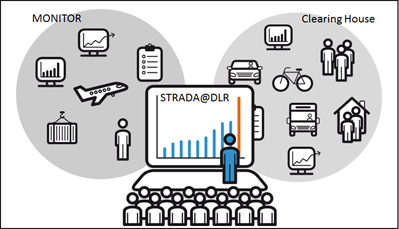
\includegraphics[width=0.8\textwidth]{strada-aproach.png}
  \caption{Aproximación del Proyecto \gls{strada} \cite{dublinstrada2}}
\end{figure}

Además de la mejora de la visualización de la información contenida, el portal ha de estar predispuesta a reforzarse y ampliarse con participación de otros institutos que aporten sus bases de datos sobre el ``Transporte y la Movilidad'' para continuar con el desarrollo del conocimiento en el \gls{dlr}.


\section{\IfLanguageName{english}{Scope}{Alcance}}
\label{section:alcance}

Este proyecto debe considerarse como un estudio piloto que establece las bases para la posible implementación usando otras fuentes de datos y permitiendo un mejor desarrollo en la gestión del conocimiento en el \gls{dlr}. Su finalidad es la mejora de la representación externa y la disposición de los datos del \gls{dlr} contribuyendo al fortalecimiento de la investigación sobre el ``\transmov''.\\

Para el público general como el especializado en los campos de política e industria se ofrecerán búsquedas avanzadas y optimizadas sobre los \glspl{metadato}, que son actualizados continuamente por los institutos involucrados. De igual forma, los usuarios deben ser atraídos por el grado de detalle y de calidad del contenido de la información proporcionada respecto a los  \glspl{metadato}. Por lo tanto, el \gls{dlr} jugará un papel importante como proveedor de servicios para la información sobre los datos incluso cuando por cuestiones de licencia estén restringidos para cierto grupos de usuarios.\\

Por este motivo, el objetivo principal de este proyecto es la creación de una nueva versión del \gls{framework} de búsqueda \gls{kf}, \gls{kf2}. Las  características más importantes del proyecto a mejorar se pueden desglosar en dos puntos principales; enriquecimiento de la visualización representando  estructuras y relaciones complejas de los datos y participación de nuevas fuentes de datos en el \gls{dlr} relacionadas con  el ``Transporte y la Movilidad''.\\
\subsection{Mejora de la visualización de estructuras y relaciones complejas de los datos}

La primera versión del proyecto \gls{kf} permite una búsqueda \gls{fulltext} sobre los datos de origen. Esta búsqueda está sólo centrada en el texto y, por lo tanto, muy limitada para los esquemas de \glspl{metadato} disponibles. Por ello, se deben diseñar e implementar para los usuarios finales unos sistemas de visualización avanzados que representen los esquemas de \glspl{metadato} dinámicos.\\

La finalidad de esta nueva visualización es la de representar las relaciones espaciales, temporales y contextuales entre los conjuntos y fuentes de datos y, por tanto, la generación de nuevos conocimientos y resultados que faciliten el proceso investigador y mejore la \gls{ux}.


\subsection{Participación de nuevas fuentes de datos en el DLR relacionadas con  el ``\transmov''}

Con el fin de aumentar el atractivo y valor del proyecto \gls{kf2} tanto dentro como fuera del \gls{dlr}, el sistema debe poder incorporar con relativa simpleza nuevas bases de datos adicionales relacionadas con el ``\transmov'' de institutos del \gls{dlr}.\\

Un claro ejemplo de estas posibilidades de mejora del conocimiento son el \gls{ts} y el \gls{fk}. Ambos poseen una base del conocimiento relacionada con el ``Transporte y la Movilidad'' y un declarado interés por contribuir a una fuente unificada de conocimiento conjunta.\\


\section{\IfLanguageName{english}{Document Structure}{Organización del
documento}} 
% \todo[inline]{Descripción de los contenidos de la presente memoria, así como del software entregado en soporte informático.}

Este documento explica el proceso de desarrollo de la aplicación \gls{kf2} y la aplicación para el portal \gls{strada}.\\

Empezando por la descripción de los objetivos iniciales y requisitos esenciales que deberá reunir dicho proyecto, 
se describe la planificación temporal del proyecto en un diagrama de \gls{gantt}, los costes estimados, estudio de los riesgos y la calidad del sistema.\\

A medida que se avance por el esta documentación, se irá explicando las fases del desarrollo del software; estudio del sistema actual y los requisitos y selección de la solución, análisis del sistema incluyendo gráficos \gls{uml} para los de casos de uso, diseño del sistema a implantar desglosado en módulos, explicación de la implementación y las pruebas realizadas.\\

Para finalizar, se incluyen los manuales necesarios para la implantación y explotación del \gls{software} y el manual para el usuario final. También se comentan las posibles mejoras o aplicaciones que pudieran considerarse en futuras versiones de este \gls{software}.
 
\chapter{\IfLanguageName{english}{Schedule}{Planificación}}
% ------------------------------------------------------------------------------
% Este fichero es parte de la plantilla LaTeX para la realización de Proyectos
% Final de Grado, protegido bajo los términos de la licencia GFDL.
% Para más información, la licencia completa viene incluida en el
% fichero fdl-1.3.tex

% Copyright (C) 2012 SPI-FM. Universidad de Cádiz
% ------------------------------------------------------------------------------

%En esta sección se describen todos los aspectos relativos a la gestión del proyecto: metodología, organización, costes, planificación, riesgos y aseguramiento de la calidad.


% \section{\IfLanguageName{english}{Organization}{Organización}}
% \label{section:organizacion}
\begin{comment}
Relación de las personas (roles) involucradas en el proyecto y de cómo se estructuran
las relaciones entre las mismas para ejecutar el proyecto. Relación de los recursos inventariables
utilizados en el proyecto: equipamiento informático (hardware y software), herramientas empleadas, etc. 
\end{comment}

\section{El Centro Aeroespacial Alemán (DLR)}
\label{section:dlr}

\begin{wrapfigure}{r}{0.3\textwidth}
  \begin{center}
    
\includegraphics[width=0.29\textwidth]{dlr-logo.jpg}
  \end{center}
  \caption{Logotipo \gls{dlr}}
\end{wrapfigure}

El \gls{dlr} es una de las instituciones públicas más importantes dedicadas a la investigación en la República Federal Alemana.\\ 

Sus oficinas centrales se encuentran en la ciudad de Colonia, más de 15 delegaciones, con 32 institutos, repartidas por el territorio nacional alemán y 5 situadas a lo largo del mundo \cite{dlrort}. Actualmente cuenta con más de 7.700 trabajadores y un presupuesto anual dependiente del \gls{bmwi}- de 157 millones de euros para el año 2014 \cite{haushalt2014}.\\


En instituciones orientadas a la investigación, como es el \gls{dlr}, la gestión del conocimiento tiene un significado muy importante. Dado el cambio de personal constante involucrado en las distintas fuentes de conocimiento, reside el peligro de pérdida del mismo. \\

La importancia de la gestión del conocimiento es debido a que éste concreta las actividades de una entidad. Estas actividades ``tienen como meta una mejora de la gestión específica de la organización tanto para el conocimiento interno como externo'' \cite{cissek}. Por lo tanto, el objetivo no debería de ser sólo el almacenamiento sino también la recuperación y reutilización del conocimiento obtenido en situaciones anteriores \cite{dengel}.\\


\subsection{``Transporte y la Movilidad'' en el DLR}

Junto con materias relacionadas con la aeronáutica, el espacio, la energía y la seguridad, el transporte es uno de sus temas de estudio, destacando la evolución de éste como unos de los puntos de trabajo más importantes. Tanto es así que 26 institutos del \gls{dlr} contribuyen en su competencia específica a la mejora del ámbito del transporte. La mayoría de ellos generan gran cantidad de conjuntos de datos estadísticos y bases de datos por lo que la gestión del conocimiento juega un papel clave en puntos como el almacenaje, descripción y su (re)utilización. En el campo de investigación sobre el trasporte y sus datos existen actualmente dos portales en el \gls{dlr}; el ``\gls{monitor}'' del \gls{fw}, implementación del \gls{framework}  \gls{kf}, que aporta datos sobre el transporte aéreo y el portal ``\cs'' del \gls{vf} contribuye con los datos sobre la investigación del transporte.


\subsubsection{\fw{}}
El foco de la investigación de este instituto es examinar cómo los dos sistemas, el tráfico aéreo y el sistema de aeropuertos, evolucionan con paso del tiempo bajo ciertas condiciones y cómo conseguir un estado deseado para cada uno. Para ello, el instituto realiza las siguientes tareas:

\begin{itemize}
  \item Analizar la situación y el desarrollo actual.
  \item Examinar la posible evolución futura de ambos sistemas, por ejemplo, a través de estudios de simulaciones.
  \item La construcción de herramientas de software para ayudar a evaluar las condiciones actuales y evitar situaciones indeseables.
  \item Desarrollar métodos para gestionar los aeropuertos de forma eficiente.
  \item Observar los efectos de las medidas aplicadas.
\end{itemize}

Por lo tanto, el objetivo de la investigación del transporte aéreo es el desarrollo de estrategias y medidas destinadas a introducir cambios en la infraestructura o las nuevas regulaciones para el sistema de transporte aéreo en su conjunto a largo plazo.\\

Tiene como objetivo la investigación del sistema aeroportuario en el desarrollo de medidas para gestionar los aeropuertos de manera eficiente. A través del estudio del movimiento de pasajeros en los procesos de la parte pública y los procesos de parte aeronáutica se intenta fomentar un transporte intermodal eficiente \cite{fwHome}.

%Tiene como objetivo la investigación del sistema aeroportuario en el desarrollo de medidas para la gestión en los aeropuertos de manera eficiente el movimiento de pasajeros en los procesos de la parte pública y la parte aeronáutica fomentando de este modo un transporte intermodal eficiente \cite{fwHome}.

\subsubsection{\vf{}}
Este instituto es el principal proveedor oficial para los hogares alemanes de encuestas y estadísticas relacionadas con el transporte. Aporta datos de sobre el trasporte público y encuestas de movilidad.\\ 

Sus investigaciones se centran en los avances y perspectivas del transporte de pasajeros y comercial para conseguir en el futuro un sistema de transporte moderno, eficiente y sostenible para las personas y el medio ambiente.\\ 

Los campos de investigación del instituto son: 
\begin{itemize}
	\item Estudios de patrones de movilidad sobre viajes domésticos y de negocios de personas.
    \item Modelos para representar y prever la demanda de trasporte regional de pasajeros y comercial.
    \item Evaluación de las tecnologías y medidas en cuanto su posible efectividad.
    \item La aceptación y uso efectivo de la red eléctrica para el trasporte de pasajeros y comercial.
    \item Las interacciones entre la información y la comunicación (TIC) con la movilidad.
\end{itemize}

Este instituto está conectado en red a través de la cooperación en investigación y proyectos a nivel nacional e internacional. Colaborando estrechamente con la docencia e investigación universitaria y la enseñanza en centros de educación superiores y de investigación \cite{vfHome}.


Los institutos \gls{vf} y \gls{fw} asignaron como personas responsables de velar por las necesidades de sus institutos, y por lo tanto de la visión proporcionada de su conocimiento por este proyecto, a varios \glspl{reshfellw}. Éstos, coordinados por el \gls{scvss}, colaboraron muy activamente en la ejecución del proyecto, proporcionando la visión de los institutos y el personal investigador que usará en un futuro la aplicación.\\

\subsection{Equipamiento informático}
Las peculiares características del \gls{dlr} ha condicionado a lo largo del proyecto fuertemente la elección de las herramientas informáticas a usar para este proyecto.

\subsubsection{Software}
Partiendo de una lista con el \gls{software} permitido en el \gls{dlr}, se han utilizado los siguientes programas:

\sparagraph{Herramientas para la gestión}
Para controlar el proceso de \gls{software} y la evolución del proyecto se han utilizado principalmente los programas mostrados en la tabla \ref{table:softgest}.

\begin{center}
\begin {table}[H]
\centering
    \begin{tabular}{ | p{3cm}  p{4cm}   p{3cm}   p{5cm} |}
    \hline
    \textbf{Software} & \textbf{Tipo} & \textbf{Versión} & \textbf{Comentario} \\ \hline
    %%%%%%
    Subversion & \Gls{software} para el control de versiones & 1.7 & Utilizado por defecto en el \gls{dlr} para el desarrollo de \gls{software} propio. \\ \hline
    MantisBT & \Gls{bugT} & 1.2 & Utilizado por defecto en el \gls{dlr} para el desarrollo de \gls{software} propio. \\ \hline
    Jenkins & \Gls{swIntcon} & 1.573 & Utilizado por defecto en el \gls{dlr} para el desarrollo de \gls{software} propio. \\ \hline
    \end{tabular}
    \caption{\Gls{software} usado para la gestión}
    \label{table:softgest}
    \end{table}
\end{center}

\sparagraph{Herramientas del entorno de desarrollo}\\
El entorno de programación donde ha implementado el proyecto se ha sustentando de la ayuda de los programas indicados en la tabla \ref{table:softdev}.

\begin{center}
\begin {table}[H]
\centering
    \begin{tabular}{ | p{3cm}  p{4cm}   p{3cm}   p{5cm} |}
    \hline
    \textbf{Software} & \textbf{Tipo} & \textbf{Versión} & \textbf{Comentario} \\ \hline
    %%%%%%
    \Gls{eclipse} & \gls{ide} & Kepler SR2 & Con los \glspl{plugin} para Subversion, MantisBT y Jenkins  \\ \hline
    Maven & Gestión y construcción de proyectos & 3.2.1 & Conjuntamente con el \gls{plugin} para Eclipse \\ \hline
    JRebel & auto-\Gls{deploy} & 5.6.1 & Conjuntamente con el \gls{plugin} para \gls{eclipse} \\ \hline
    \end{tabular}
    \caption{\Gls{software} usado como entorno de desarrollo}
    \label{table:softdev}
  \end{table}
\end{center}

\sparagraph{Herramientas usadas para el desarrollo}
El producto resultado de este proyecto requiere o ha necesitado en alguna de sus etapas de desarrollo el \gls{software} listado en la tabla \ref{table:softdevsw}.

\begin{center}
\begin {table}[H]
\centering
    \begin{tabular}{ | p{3cm}  p{4cm}   p{3cm}   p{5cm} |}
    \hline
    \textbf{Software} & \textbf{Tipo} & \textbf{Versión} & \textbf{Comentario} \\ \hline
    %%%%%%
    \Gls{java} & Lenguaje de programación & 1.7 & Lenguaje conocido ampliamente por \gls{scvss} \\ \hline
    Wiremock & \Gls{framework} para \gls{sw} & 1.18 & \Gls{mocking} web services \\ \hline
    Spring & \Gls{framework} para la web& 4.0.3 & Conjuntamente con el \gls{plugin} para \gls{eclipse} \\ \hline
    Jackson & Librería \Gls{java}& 1.9.13& Libreria para tratar documentos \gls{json} \\ \hline
    SLF4J & Librería \Gls{java}& 1.9.13& Systema de \gls{logging} \\ \hline
    \end{tabular}
    \caption{\Gls{software} usado para desarrollar el programa}
    \label{table:softdevsw}
  \end{table}
\end{center}

\sparagraph{Herramientas usadas para la fase de \gls{testing}}
Para comprobar el correcto funcionamiento y asegurar la calidad del producto final se han utilizado las herramientas de \gls{software} indicadas en la tabla \ref{table:softtest}.

\begin{center}
\begin {table}[H]
\centering
    \begin{tabular}{ | p{3cm}  p{4cm}   p{3cm}   p{5cm} |}
    \hline
    \textbf{Software} & \textbf{Tipo} & \textbf{Versión} & \textbf{Comentario} \\ \hline
    %%%%%%
    Powermock & Librería \Gls{java} & 1.4 & Usado para simular comportamientos en los test \\ \hline
    EasyMock & Librería \Gls{java} & 3.2 & Usado para simular comportamientos en los test \\ \hline
    JUnit & Librería \Gls{java}  & 4.12& Herramienta de \gls{testing}  de \Gls{java} \\ \hline
    \end{tabular}
    \caption{\Gls{software} usado durante la fase de \gls{testing}}
    \label{table:softtest}
  \end{table}
\end{center}

\sparagraph{Herramientas usadas para el \gls{despliegue}}
El \gls{software} de la tabla \ref{table:sofdesp} fue utilizado tanto durante el desarrollo como en el servidor de pruebas donde reside el proyecto para comprobar en todo su conjunto el correcto funcionamiento y como demostración.

\begin{center}
\begin {table}[H]
\centering
    \begin{tabular}{ | p{3cm}  p{4cm}   p{3cm}   p{5cm} |}
    \hline
    \textbf{Software} & \textbf{Tipo} & \textbf{Versión} & \textbf{Comentario} \\ \hline
    %%%%%%
    \gls{liferay} & Portal de gestión de contenidos & 6.2.1 CE GA2 & Utilizado junto sus \glspl{plugin} para \gls{eclipse} durante el desarrollo \\ \hline
    \gls{tomcat} & Servidor web & 7 &  Usado conjuntamente con gls{liferay} \\
    \hline
    \gls{solr} & \Gls{motorbusqueda}& 4.8.1& \Gls{motorbusqueda} desarrollado en \Gls{java}\\ \hline
    \gls{jetty} & Servidor web & 7& Usado conjuntamente con \gls{solr} \\ \hline
    \end{tabular}
    \caption{\Gls{software} usado para el \gls{despliegue} de la aplicación}
    \label{table:sofdesp}
  \end{table}
\end{center}

\sparagraph{Herramientas usadas para documentación}
Para generar la presente documentación se han utilizado las herramientas expuestas en la tabla \ref{table:softdoc}.

\begin{center}
\begin {table}[H]
\centering
    \begin{tabular}{ | p{3cm}  p{4cm}   p{3cm}   p{5cm} |}
    \hline
    \textbf{Software} & \textbf{Tipo} & \textbf{Versión} & \textbf{Comentario} \\ \hline
    %%%%%%
    write\LaTeX{} & Editor online &  & Editor web para \gls{latex} \\ \hline
    GanttProject & Editor de gráficos & 2.5& Herramienta para la generación de gráficos de \Gls{gantt} \\ \hline
    Gimp & Editor de imágenes &  2.8.10 & Edición de imágenes muy completo \\ \hline
    ConceptDraw & Editor de gráficos &  10  & Edición de gráficos \gls{uml} \\ \hline
    \end{tabular}
    \caption{\Gls{software} usado para la generación de la documentación}
    \label{table:softdoc}
  \end{table}
\end{center}


\sparagraph{Herramientas usadas para la comunicación y coordinación}
Dado el carácter distribuido y descentralizado de los departamentos en el \gls{dlr} y la distancia física que separan cada uno de los agentes implicados en el proyecto, las herramientas de comunicación usadas son un factor clave durante el desarrollo del proyecto, tabla \ref{table:softcomu}.

\begin{center}
\begin {table}[H]
\centering
    \begin{tabular}{ | p{3cm}  p{4cm}   p{3cm}   p{5cm} |}
    \hline
    \textbf{Software} & \textbf{Tipo} & \textbf{Versión} & \textbf{Comentario} \\ \hline
    %%%%%%
    Lync & Servicio de \gls{mensinst} & 4.0.7 & Usado en \gls{dlr} como sistema oficial de comunicación entre los trabajadores \\ \hline
    Outlook & Organizador personal & 14.0.7& Usado en \gls{dlr} como sistema de correo y calendario\\ \hline
    Confluence & \Gls{wiki} & 5.5& \Gls{wiki} para alojar la documentación de los proyectos desarrollados en \gls{dlr} \\ \hline
    \end{tabular}
    \caption{Herramientas usadas para la comunicación y coordinación}
    \label{table:softcomu}
  \end{table}
\end{center}

\subsubsection{\Gls{hardware}}
En lo referente al \gls{hardware}, se distinguen dos máquinas únicamente; la dedicada a la implementación del producto y un servidor usado como máquina de pruebas.

\sparagraph{\Gls{hardware} para el desarrollo}
A continuación se muestra en el cuadro \ref{table:harddev} la información del \gls{hardware} utilizado para el desarrollo del proyecto.


\begin{center}
\begin {table}[H]
\centering
    \begin{tabular}{ | r | r |}
    \hline
    S.O.& Windows 7 \\ \hline
    Procesador & Intel Core 2 Duo P8600 - 2.4GHz \\ \hline
    Memoria RAM & 4 GB \\ \hline
    Pantalla & 15.4" + 22" \\ \hline
    Disco Duro & 500GB \\ \hline
    Tarjeta Gráfica & Intel Graphics Media Accelerator (GMA) 4500MHD \\ \hline
    \end{tabular}
    \caption{\Gls{hardware} del equipo usado para el desarrollo}
    \label{table:harddev}
  \end{table}
\end{center}


\sparagraph{\Gls{hardware} del servidor}
Las propiedades del servidor gestionado por \gls{dlr} donde reside la aplicación de prueba se muestran en la tabla \ref{table:hardserv}.

\begin{center}
\begin {table}[H]
\centering
    \begin{tabular}{ | r | r |}
    \hline
    S.O.& Ubuntu 12.04.04 TLS \\ \hline
    Procesador & Intel® Xeon® Processor E5-2660 \\ \hline
    Memoria RAM & 4 GB \\ \hline
    Disco Duro & 500GB \\ \hline
    \end{tabular}
	\caption{\Gls{hardware} del servidor para la aplicación de pruebas}
    \label{table:hardserv}
  \end{table}
\end{center}

\section{\IfLanguageName{english}{Development Methodology}{Metodología de desarrollo}}

\begin{comment}Definición del proceso de desarrollo, ciclo de vida y metodología empleada durante la elaboración del proyecto. Las fases y/o iteraciones que proponga el método empleado deberán quedar recogidas en la planificación que se detalle más adelante.
\end{comment}

Las fases iniciales del proyecto pueden dividir en los siguientes puntos:

\begin{itemize}
\sitem{Estudio del proyecto \gls{kf}}
La primera fase del proyecto consistió en un estudio exhaustivo de la documentación y la implementación del proyecto predecesor. También se produjeron varias reuniones con los miembros del \gls{scvss} para perfilar los aspectos menos nítidos y confusos del funcionamiento e implementación de \gls{kf}.

\sitem {Estudio de las nuevas necesidades de visualización}
Una vez estudiado y comprendido la situación de la que se partía, se estudiaron las distintas posibilidades de visualización y de interacciones de los usuarios sobre los datos. Todo esto teniendo siempre presente la \gls{ux} como punto clave del estudio. 
% \question{alargar el punto para explicar más? en requisitos? toma de decisiones?}

\sitem{Estudio de las tecnologías disponibles para la visualización}
Para comprobar qué tecnologías son las más apropiadas para obtener una visualización acorde a las necesidades del proyecto y del usuario, se estudiaron un amplio conjunto de tecnologías y opciones de aplicación.\\ 
% \question{alargar el punto para explicar más? en requisitos? toma de decisiones?}
% \todo{alargar punto para incluir las entrevistas y el proceso de estudio con anexo}

\sitem{Estudio de la capa de servicios}
Durante los estudios previos explicados anteriormente, se detectaron grandes dificultades para cubrir los objetivos del proyecto (ver capítulo  \ref{chapter:requisitos}). Esto condicionó que una parte de la aplicación, la implementación capa de servicios, tuviera que replantearse 
%\todo{explicarlo mejor\\ en otra parte\\ del documento\\ o aquí en un\\ apartad} 
en conformidad con la gestión de proyectos en el \gls{scvss} y las necesidades de los institutos \gls{fw} y \gls{vf}.

\end{itemize}

Una vez obtenida toda la información necesaria para el planteamiento del proyecto, se optó por un proceso de desarrollo basado en \glspl{prototipo}, en concreto ``\gls{extreprot}'' \cite{extrPro}\cite{extreprobook} dada su adaptabilidad a las posibles diferentes decisiones a tomar.

\subsubsection{Aplicando ``\gls{extreprot}''}
\label{subsubsection:aplicandoextre}
El ``\gls{extreprot}'' es un proceso para desarrollar aplicaciones, especialmente aplicaciones web, basada en el diseño de \glspl{prototipo} funcionales cada vez más complejos. Este proceso se divide en cuatro fases: 
% \todo{incluir estos pasos para comparar en las conclusiones cuanto tiempo se ha gastad de más}
\begin{itemize}
\sitem{Static Prototype phase} La primera fase consiste en un \gls{prototipo} estático, implementado normalmente \gls{html}. En el caso de este proyecto se optó por bocetos en soporte físico con ejemplos reales implementados en \gls  {html} y \gls{js} para ilustrar a su vez las posibilidades de interacción de los usuarios y comportamiento del producto futuro.

\sitem{Extended Static Prototype phase} En siguiente fase de \gls{extreprot}  se define el modelo lógico de los datos. Los datos provienes de la capa de servicio son definidos. Para el proyecto \gls{kf2} se definió los valores para el índice de búsqueda.

\sitem{Extreme Prototype phase} La tercera fase se apoya la implementación de un \gls{prototipo} dinámico usando el \gls{framework} de programación deseado. Este \gls{prototipo} es totalmente funcional sustentando su funcionamiento en una capa de servicios simulada. Al concluir esta fase, la \gls{ui} quedó definida y su futuro funcionamiento demostrable. 
% \question{Explicar Wiremock? o como se simulo los servicios?}

\sitem{Service Implementation Phase} La última fase del \gls{extreprot}  consiste en la implementación de los servicios anteriormente simulados. Junto con el \gls{prototipo} de la fase anterior y algunos cambios de adaptación se consiguió la integración de todos los componentes implementados anteriormente. 
%\question{Explicar la implementación de los servicios?}
\end{itemize}

En la imagen \ref{image:extreprot} se expone los fundamentos de esta metodología.\\

\begin{figure}[h!]
  \centering
     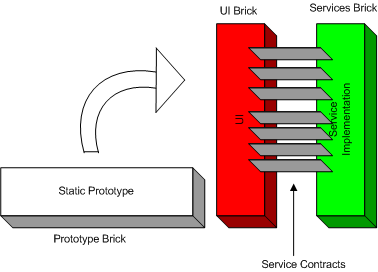
\includegraphics[width=0.6\textwidth]{extreme-prototyping-3-bricks.png}
  \caption{Los tres ``bricks'' o \glspl{prototipo} de \gls{extreprot} \cite{extrPro}}
  \label{image:extreprot}
\end{figure}

Como fase final del presente proyecto se realizaron algunos cambios simples a petición de los institutos \gls{vf} y \gls{fw}. Estos cambios para sirvieron  para precisar el producto obtenido en las anteriores fases. De esta forma, el producto obtenido final a través del \gls{extreprot} cumplió satisfactoriamente las  necesidades planteadas.

\section{\IfLanguageName{english}{Project's Schedule}{Planificación del
proyecto}} 
La planificación inicial del proyecto se puede observar en el diagrama de \gls{gantt} \ref{image:ganttinicial}. En ella se pueden diferenciar la planificación inicial para las distintas fases del desarrollo.\\

No obstante, durante la decisión de la visualización se acordó junto con el \gls{scvss} una replanificación del proyecto alargando su fases de desarrollo y la duración del conjunto del proyecto. Estas modificaciones se observan el la gráfica de \gls{gantt} \ref{image:ganttrepla}.

\begin{comment}
\todo[inline]{Estimación temporal y definición del calendario básico (hitos principales e iteraciones). Desarrollo de la planificación detallada, utilizando un diagrama de Gantt. Los diagramas de Gantt que se vean correctamente (girados y divididos si hace falta).}

En la imagen \ref{image:gantt} se muestra las fases del proyecto temporalmente ordenadas y las relaciones de dependencia entre ellas.
\end{comment}

\begin{figure}
\centering
\begin{minipage}{.5\textwidth}
  \centering
     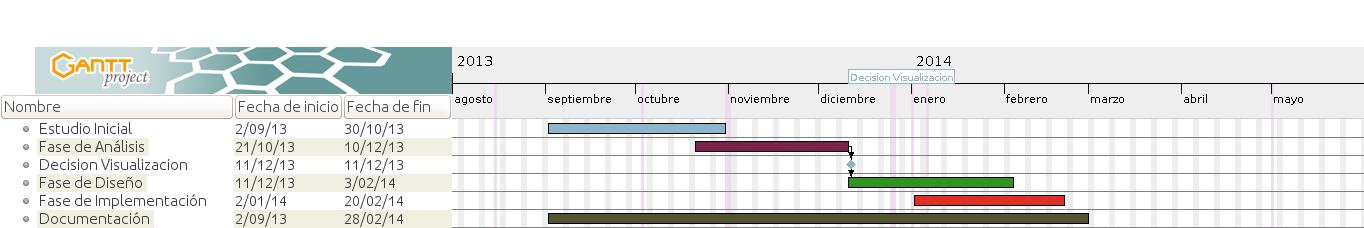
\includegraphics[width=2.5\textwidth, angle=90]{gantt-inicial.png}
  \captionof{figure}{Gráfica inicial de Gantt}
  \label{image:ganttinicial}
\end{minipage}%
\begin{minipage}{.5\textwidth}
  \centering
     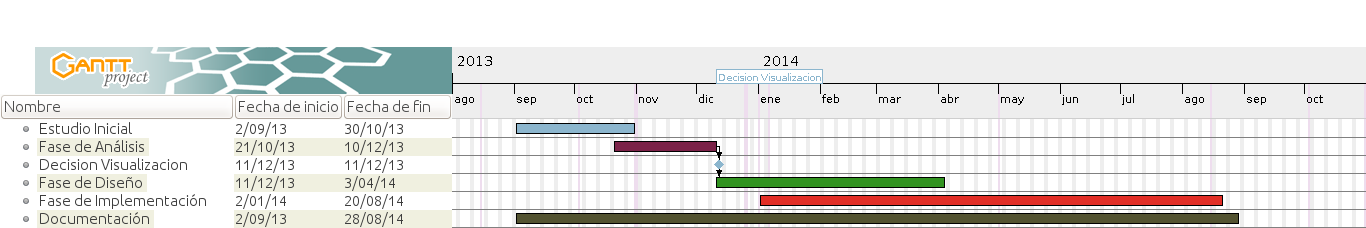
\includegraphics[width=2.5\textwidth, angle=90]{gantt-replanteamiento.png}
  \captionof{figure}{Gráfica de Gantt de la replanificación}
  \label{image:ganttrepla}
\end{minipage}
\end{figure}

%\todo[inline]{
% Se debe incluir una comparación cuantitativa del tiempo y el esfuerzo realmente invertido frente al estimado y planificado. Estos datos pueden recogerse del sistema de gestión de tareas empleado para el seguimiento del proyecto.}\question{cómo hacer la comparación cuantitativa??}

\section{\IfLanguageName{english}{Cost Estimation}{Costes}}
Los costes de este proyecto son principalmente coste de personal. Esto abarca tanto el coste proporcional al salario de cada trabajador del \gls{dlr} que interviene durante el proceso (\gls{vf}, \gls{fw}, \gls{scvss}, personal administrativo del \gls{dlr}, \dots) como los gastos derivados de las reuniones realizas para su realización (dietas, viajes, \dots).\\

Además habría que incluir el uso de las infraestructuras y recursos tecnológicos (\gls{hardware} y \gls{software}) necesitados.\\

Lamentablemente, dada la naturaleza del \gls{dlr}, esta información no puede ser publicada al igual que el presupuesto de partida para este proyecto. En cambio podremos realizar una estimación del coste del proyecto teniendo en cuenta los anteriores factores.\\

\subsection{Estimación}

Si suponemos que el equipo utilizado tiene un coste de 1512\euro{} para un periodo de amortización de tres años se tiene que el coste por mes usado es de 42\euro{}. El mobiliario utilizado y el servidor junto con la infraestructura pertenecen al \gls{dlr} pero implica también tenga un coste relacionado al proyecto, suponemos que asciende a 300\euro{} al mes junto con otros gastos relacionados con el mobiliario (luz, agua, \dots) .\\


El proyecto tiene una estimación temporal de once meses, suponiendo que el desarrollador dedica unas 20 horas semanales, hasta la finalización del proyecto, hace un total de 880 horas (11 meses a 4 semanas por mes). Para las reuniones se estima que se necesitan 40 horas para todos \glspl{reshfellw} y 20 horas de personal administrativo (tabla \ref{table:salmes}).\\

\begin{center}
\begin {table}[H]
    \begin{tabular}{ | l | c | p{6.5cm} |}
    \hline
    \textbf{Cargo} & \textbf{Coste} & \textbf{Descripción} \\
    				& (persona/mes) &                      \\ \hline
    Desarrollador & 5.5 persona/mes & Desarrollador sin experiencia (realiza el producto)\\ \hline
    \gls{reshfellw} & 0,25 persona/mes& Colabora activamente \\ \hline
    Personal administrativo  & 0,125 persona/mes& Gestión de personal y proyectos \\ \hline
    \end{tabular}
    \caption{Resumen del gasto de personal}
    \label{table:salmes}
  \end{table}
\end{center}

Los salarios del personal del \gls{dlr} es público al ser una institución dependiente del Estado. Por lo tanto, partiendo de la tabla de salarios públicos \cite{tvod} obtenemos los datos relevantes para la estimación resumidos en la tabla \ref{table:resucost}. También se destina una partida de 2000\euro{} para reuniones y gastos variados.\\

De forma complementaria, en la tabla \ref{table:resucost} también se muestran los cálculos con los salarios medios obtenidos de la herramienta on-line de Infojobs \cite{infojobs}.\\

Calculando la estimación de todos las variables anteriormente expuestas se obtiene una estimación de 23647,88\euro{}  (13963,94\euro{} en España ).

\begin{center}
\begin {table}[H]
    \begin{tabular}{ |l|c|c|c|c|c|}
    \hline
    \textbf{Recurso} & \textbf{Número de } & \textbf{Precio/unidad } & \textbf{Precio/unidad } & \textbf{Total} & \textbf{Total} \\ 
      & unidades & Alemania(\euro{}) & España(\euro{}) & Alemania(\euro{}) & España(\euro{})\\ \hline
    %%%%%%%
    Desarrollador & 5,5 & 2.965 & 1351,75 & 16307,5 & 7434,625 \\ \hline
    \gls{reshfellw} & 0.25 & 4.558 & 2.254,08 & 1139,5 & 563,5\\ \hline
    Admon. & 0,125 & 3.519 & 1.630,5 & 439,875 & 203,8125\\ \hline
    Equipo & 11 & 42\euro{} & 42\euro{} & 462 & 462 \\ \hline
    Infraestructura & 11 & 300 & 300 & 3300 & 3300 \\ \hline
    Variados & 1 & 2000 & 2000 & 2000& 2000 \\ \hline\hline
    TOTAL &&&& 23647,88 & 13963,94 \\ \hline
    \end{tabular}
    \caption{Resumen de la estimación de los costes}
    \label{table:resucost}
  \end{table}
\end{center}




% \review{Cuenta los costes no reales que estimarías si el proyecto se hiciera en España, incluyendo costes de amortización de equipos y costes de personal según alguna tabla salarial estándar (de la UCA, de infojobs, etc.)}

\begin{comment}
\question{qué puedo poner? algo más?}
\todo[inline]{
Estudio y presupuesto de los costes de los recursos (humanos y materiales) descritos anteriormente, necesarios para el proyecto.

Para el cálculo de costes de personal pueden consultarse las tablas salariales de la UCA para el personal técnico de apoyo contratado laboral \cite{makebst}, o bien otras más ajustadas a la realidad. El cálculo del coste del personal del proyecto debe hacerse en personas-mes, y luego hacer la correspondencia al coste monetario.\\
}
\end{comment}
\section{\IfLanguageName{english}{Risks Estimation}{Riesgos}}
%Enumeración de los riesgos del proyecto, indicando su posible impacto (efecto que la ocurrencia del citado riesgo tendría en el desarrollo del proyecto) y la probabilidad de ocurrencia. Una vez los riesgos son identificados y priorizados, hay que definir los planes necesarios para reducir los efectos del riesgo una vez se haya materializado o disminuir que este ocurra.

En todo proyecto \gls{software} se pueden producir situaciones que difcultarían el proceso de desarrollo, el cumplimiento de los plazos establecidos o desajustarían el presupuesto asignado. Estos riesgos pueden ser causados por numeroso factores de distinta naturaleza. Por ello es necesario el estudio previo de éstos.\\

Utilizando como base MAGERIT versión 3 \cite{MAGERIT}, se van a describir un conjunto de posibles riesgos genéricos y específicos para el desarrollo del proyecto \gls{kf2}.\\

\subsection{Descripción de Riesgos}
En los siguientes puntos se describen los riesgos junto con su valoración del impacto y probabilidad de ocurrencia usando las tablas \ref{table:valoracion} y \ref{table:probabilidad}.

\begin{center}
\begin {table}[H]
\centering
    \begin{tabular}{ | r | r |}
    \hline
\textbf{Valoración} & \textbf{Descripción}  \\ \hline
MB &  Impacto muy bajo \\ \hline
B & Impacto bajo \\ \hline
M & Impacto medio\\ \hline
A & Impacto alto \\ \hline
MA & Impacto muy alto \\ \hline
    \end{tabular}
	\caption{Tabla valoración impacto de riesgos}
    \label{table:valoracion}
  \end{table}
\end{center}

\begin{center}
\begin {table}[H]
\centering
    \begin{tabular}{ | r | r |}
    \hline
\textbf{Ocurrencia} & \textbf{Descripción} \\ \hline
Muy Frecuente(MF) & A diario \\ \hline
Frecuente(F) & Una vez al mes \\ \hline
Frecuencia Normal(FN) & Una vez al año \\ \hline
Poco Frecuente(PF) & Cada varios Años \\ \hline
    \end{tabular}
	\caption{Tabla probabilidad riesgos}
    \label{table:probabilidad}
  \end{table}
\end{center}


\subsubsection{Riesgos genéricos}
Estos tipos de riesgos son comunes para el desarrollo de todo proyecto software:
\begin{enumerate}[label=\bfseries G\arabic*]
	\sitem{Riesgos de servicios (B-FN)}
    Representan la problemática posible causada por la prestación de servicios internos. 
    \sitem{Pérdida de información y datos (MA-PC)}
    Corrupción o pérdida total de los datos almacenados para el proyecto.
    \sitem{Fallos del \gls{software}(A-FN)}
	Problemas causados por errores o fallos del \gls{software}.
    \sitem{Problemas con el \gls{hardware} (MA-PC)}
    Problemas con los elementos físicos usados (ordenadores, impresoras, \dots).
    \sitem{Problemas de personal (M-F)}
    Indisposición inesperada de alguno de los recursos humanos disponibles relacionados con el proyecto.
    \sitem{Problemas de red (FN-M)}
    Fallo de la conexión de los sistemas de comunicación (teléfono, internet, \dots).
\end{enumerate}

\subsubsection{Riesgos específicos}
Los riesgos particulares del presente proyecto son:

\begin{enumerate}[label=\bfseries E\arabic*]
	\sitem{Cambio del origen de datos (A-FN)}
	Si es necesario obtener los datos desde otro sistema de almacenamiento (base de datos, ficheros \gls{xml}, \dots) habría que modificar el sistema de importación para una correcta obtención de éstos.
    
	\sitem{Cambio en el formato del origen de datos (A-FN)}
    Si se modificara la especificación del formato de los datos obtenidos, habría que modificar el sistema de extracción de los mismos.
    
    \sitem{Variación del sistema de información (A-MF)}
    A lo largo de la vida del proyecto, las necesidades del sistema de información pueden variar.
    
    \sitem{Modificación del funcionamiento de la visualización (A-MF)}
    El sistema de visualización puede cambiar obligando al uso o modificación de nuevos Componentes  visuales.
\end{enumerate}

\subsection{Subsanación de los Riesgos}    
El departamento \gls{scvss} dispone de un servidor con \gls{svn}. Usando este sistema a de control de versiones se subsanarán los riesgos que provocan una pérdida de datos (G2-4). Este servidor reside en las instalaciones de T-Systems con copias de seguridad diariamente programadas.\\

Los posibles problemas causados por los riesgos de personal (G5) implican, sobre todo, el replanteamiento de las reuniones con las personas involucradas del \gls{dlr}. Usando una planificación de reuniones a largo plazo con posibles alternativas se evitan, en su mayoría, la repercusión en el proyecto. Respecto al equipo de desarrollo, éste se compone solamente de una persona por lo que este riesgo queda considerablemente acotado en sus efectos y sus posibles opciones para resarcirlo.\\

Para desagraviar los riesgos específicos de la aplicación (E1-4), durante el proceso de desarrollo se ha de estar en contacto directo con el entorno interesado en el proyecto (\textit{Stackeholders}).

\section{\IfLanguageName{english}{Quality Assurance}{Aseguramiento de calidad}}
% \question{qué puedo poner? SVN, Mantis, wiki, jenkins?? testing??}

\begin{comment}
En esta sección se incluirán las actividades y tareas relacionadas con el aseguramiento de calidad a realizar durante el desarrollo del software. Se incluirán los estándares, prácticas y normas aplicables durante el desarrollo del software.\\

También, deberán recogerse los diferentes tipos de revisiones, verificaciones y validaciones que se van a llevar a cabo, los criterios para la aceptación o rechazo de cada producto y los procedimientos para implementar acciones correctoras o preventivas.
\end{comment}
Para asegurar la calidad del proceso de desarrollo y llevar un control sobre el mismo se debe utilizar el \gls{software} \gls{mantis} en conexión con los \textit{commits} realizados en \gls{svn}. Para ello se obliga a que cada \textit{commit} ejecutado esté relacionado con un ticket o tarea previamente definida en \gls{mantis}.\\

La documentación del proyecto generada debe accesible y verificable por el resto de miembros del \gls{scvss} a través de una \gls{wiki} interna.\\

La calidad del código fuente adquiere una relevancia muy alta para asegurar el mantenimiento del \gls{software}. Para ello, hay que prestar especial atención durante el desarrollo en los siguientes aspectos:

\begin{itemize}
	\item Código claro y estructurado.
    \item Utilización de patrones de diseño.
    \item Utilización de estándares de codificación para \gls{java} \cite{javacode}, \gls{js} \cite{javascriptcode} y \gls{html} \cite{htmlcode}.
    \item Código moderadamente comentado.
    \item Utilización de ficheros de configuración.
\end{itemize} 

A través de \gls{testing} se debe asegurar el correcto funcionamiento de la aplicación en sus aspectos más importantes. Junto con \gls{jenkins}, se debe realizar la integración e inspección continua.




\textbf{}

% DESARROLLO
\part{\IfLanguageName{english}{Development}{Desarrollo}}
\null\vfill

\chapter{\IfLanguageName{english}{System Requirements}{Requisitos del Sistema}}
% ------------------------------------------------------------------------------
% Este fichero es parte de la plantilla LaTeX para la realización de Proyectos
% Final de Grado, protegido bajo los términos de la licencia GFDL.
% Para más información, la licencia completa viene incluida en el
% fichero fdl-1.3.tex

% Copyright (C) 2012 SPI-FM. Universidad de Cádiz
% ------------------------------------------------------------------------------
\begin{comment}
En esta sección se detalla la situación actual de la organización y las necesidades de la misma, que originan el desarrollo o mejora de un sistema informático. Luego se presentan los objetivos y el catálogo de requisitos del nuevo sistema. Finalmente se describen las diferentes alternativas tecnológicas y el análisis de la brecha entre los requisitos planteados y la solución base seleccionada, si aplica.
\end{comment}

\label{chapter:requisitos}

\section{\IfLanguageName{english}{Current Situation}{Situación actual}}
\begin{comment}
Esta sección debe contener información sobre la situación
actual de la organización para la que se va a desarrollar el sistema software.
\end{comment}
Como se ha explicado anteriormente en el capítulo \ref{chapter:introduccinon}, el presente proyecto nació con la necesidad de mejoras del \gls{framework} de búsqueda \gls{kf} aplicándose como modelo piloto al proyecto \gls{strada}.

\begin{comment}
\question{que situación actual de la organización y las necesidades de la misma, que originan el desarrollo o mejora de un sistema informático?? expuesto en la introducción \ref{section:alcance}}
\end{comment}

\subsection{\IfLanguageName{english}{Business Process}{Procesos de Negocio}}
\begin{comment}
Esta sección debe contener información sobre los modelos de procesos de negocio actuales, que suelen ser la base de los modelos de procesos de negocio a implantar.
\end{comment}

A continuación se detallan los procesos de negocio principales del proyecto \gls{kf} que actualmente están implantados.

\subsubsection{Importación de los datos}
En este proceso de negocio se produce la importación de los datos provenientes de un único repositorio de \gls{svn}. En el proceso implantado es necesario tanto permisos para poder obtener los datos del repositorio remoto como una copia local, previamente descargada. En la imagen \ref{image:negimport1} se representa el modelo proceso de este negocio en \gls{uml}.

\begin{figure}[H]
  \centering
    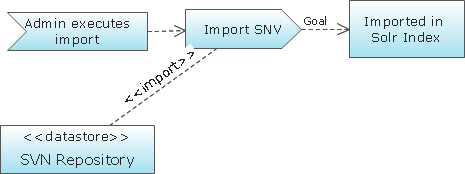
\includegraphics[width=0.8\textwidth]{NegocioOldImport.png} 
  \caption{Modelo de proceso de negocio, importación de los datos en \gls{kf}}
  \label{image:negimport1}
\end{figure}

\subsubsection{Búsqueda en el portal}
Este proceso de negocio se produce cuando el usuario filtra el conjunto de documentos usando para ello la interfaz web. Como resultado de la acción, el usuario obtiene una lista acorde con el filtro aplicado.  En la imagen \ref{image:negsearch1} se representa el modelo proceso de este negocio en \gls{uml}.

\begin{figure}[H]
  \centering
    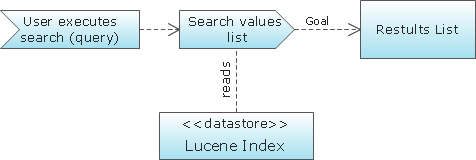
\includegraphics[width=0.8\textwidth]{NegocioOldSearch.png} 
  \caption{Modelo de proceso de negocio, búsqueda en el portal \gls{kf}}
  \label{image:negsearch1}
\end{figure}


\subsection{\IfLanguageName{english}{Technological Environment}{Entorno
Tecnológico}}
\begin{comment}
Esta sección debe contener información general sobre el entorno tecnológico en la organización del cliente antes del comienzo del desarrollo del sistema software, incluyendo hardware, redes, software, etc.
\end{comment}
\label{subsection:entornotech}

\sparagraph{Construcción}
La versión de la que se parte de \gls{kf} está implementada usando \Gls{jsdk} 6 Update 45 y \gls{maven} para la construcción del producto unificando todas sus partes, en la figura \ref{image:mavenkf} se puede observar un esquema de la organización de los archivos de configuración de \gls{maven} para esta versión del proyecto.\\

\begin{figure}[H]
  \centering
    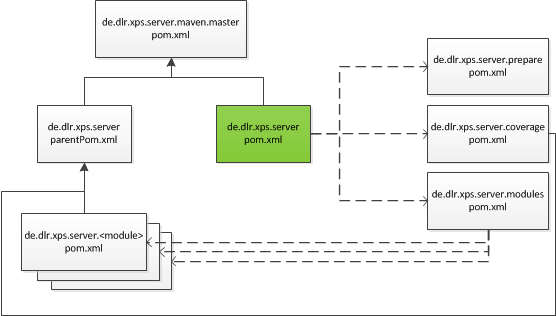
\includegraphics[width=0.8\textwidth]{DevDoc_PomStructure.png}
  \caption{Estructura simplificada de \gls{maven} en \gls{kf}}
  \label{image:mavenkf}
\end{figure}

Dado el portal donde se aloja la información de los institutos a los que está destinado \gls{kf} es \gls{liferay}, para esta versión del proyecto se implementó como contenedor un \gls{portlet} para \gls{liferay} 6.1 CE GA2 (6.1.1) sobre un servidor \gls{tomcat} 6.

\sparagraph{Importación}
A través de la lectura del repositorio remoto una copia local se extraen los dados de los documentos y se genera un índice de búsqueda en la fase de importación. Éste es índice es una instancia de \gls{lucene} en su version 3.0.2.\\

\sparagraph{Índice de búsqueda}
Partiendo de los datos del portal \gls{cs} (imagen \ref{image:csdata}) y del portal \gls{monitor} (imagen \ref{image:modata}) se crea durante la importación de los datos un índice de búsqueda con las propiedades expuestas en la imagen \ref{image:stradadata} para la instancia \gls{strada} del \gls{framework} \gls{kf} usada como referencia \cite{dublinstrada}.


\begin{figure}[H]
  \centering
    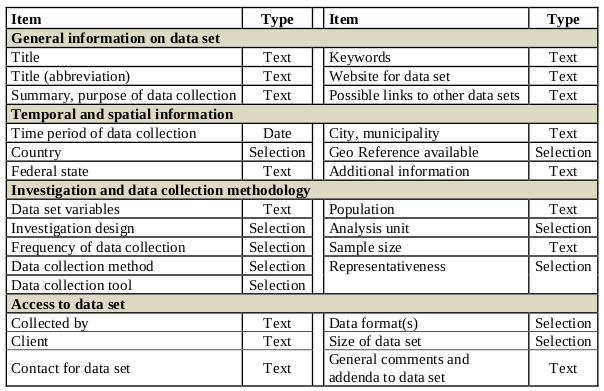
\includegraphics[width=0.8\textwidth]{cs_dublin.png} 
  \caption{\Glspl{metadato} de \gls{cs} \cite{dublinstrada}}
  \label{image:csdata}
\end{figure}

\begin{figure}[H]
  \centering
    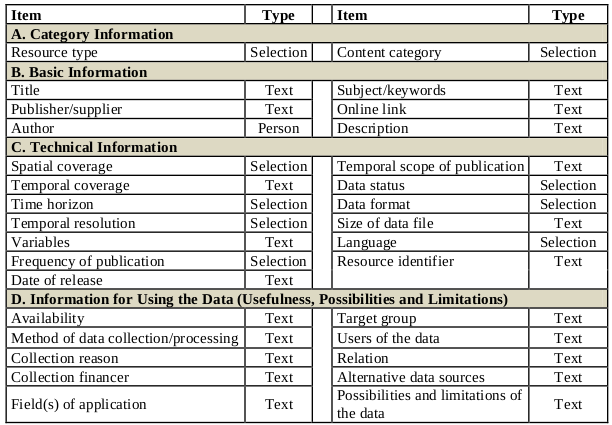
\includegraphics[width=0.8\textwidth]{monitor_dublin.png} 
  \caption{\Glspl{metadato} de \gls{monitor} \cite{dublinstrada}}
  \label{image:modata}
\end{figure}

\begin{figure}[H]
  \centering
    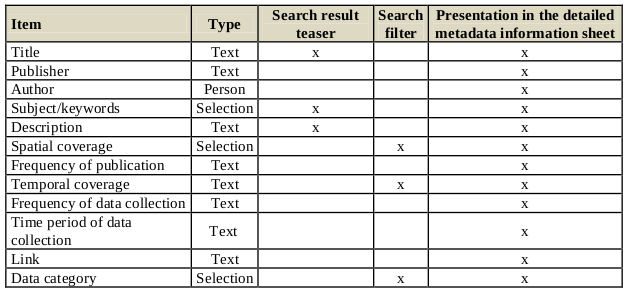
\includegraphics[width=0.8\textwidth]{strada_dublin.png} 
  \caption{\Glspl{metadato} de \gls{strada} \cite{dublinstrada}}
  \label{image:stradadata}
\end{figure}

\sparagraph{Interfaz de usuario}
Para la realización de la página web se utilizó el \gls{framework} de programación web  \gls{vaadin} 6. Únicamente usando sus componentes predefinidos se implementó la interfaz de usuario y su funcionalidad.\\

Junto con la configuración de un tema de \gls{liferay} por cada instancia del \gls{framework} (\gls{elib}, \gls{monitor} y \gls{strada}del se terminó de perfilar la apariencia y el comportamiento de la interfaz.

\sparagraph{Configuración}
Exceptuando la importación de los datos que se configura a nivel de parámetros en la ejecución, la configuración y adaptación del \gls{kf} para los distintos escenarios se realiza a nivel de código, es decir, que para cada instancia que se implemente hay que editar el \gls{framework} para adaptarlo a las necesidades específicas requeridas.


\subsection{\IfLanguageName{english}{Weakness and Strong Points}{Fortalezas y Debilidades}}
\begin{comment}
Esta sección debe contener información sobre los aspectos positivos y negativos del negocio actual de la organización para la que se va a desarrollar el sistema software.
\end{comment}
La implementación del \gls{framework} \gls{kf} presenta unos aspectos positivos y negativos que se pueden agrupar en los siguientes puntos:

\begin{itemize}
\sitem{Importación de los datos y el índice de búsqueda}
Como anteriormente se ha comentado, para la importación de los datos en el índice de \gls{lucene} es necesario contar con una copia local del repositorio \gls{svn} y acceso al repositorio remoto. Esto representa un gran inconveniente durante la fase de desarrollo ya que el repositorio remoto es no debería de tener que ser modificado con datos de prueba durante el desarrollo.\\

Al obtener los datos también remotamente, el proceso de importación de los datos es dependiente tener acceso a este repositorio. Esto conlleva que el tiempo necesario para finalizar esta tarea se incremente notablemente y que el desarrollador siempre tenga que tener acceso a la red. En el código \ref{code:importkf1} se muestra un ejemplo de ejecución para importar los datos usando la linea de comandos. Por otra parte, esta simpleza hace que la importación se pueda ejecutar desde la linea de comandos o, por ejemplo, desde algún sistema automático como \gls{cron}.

\begin{listing}
\begin{minted}[linenos,
               numbersep=5pt,
               frame=single,
               framesep=2mm]{bash}
               
java -Xmx512m -jar
de.dlr.xps.server.datafinder.indexer.fw-jar-with-dependencies.jar 
--idx-path D:\Projects\xps\index\fw-test-data
--svn-username user 
--svn-password ********
--svn-url https://svn.sistec.dlr.de/svn/xps/fw-test-data/ 
--svn-working-copy-path "D:\Repositories\fw-test-data\data\dat" 
--parse-content

	\end{minted}
	\caption{Ejemplo de importación de datos en \gls{kf}.}
	\label{code:importkf1}
\end{listing}


\sitem{Configuración de las nuevas instancias}
Cada instancia del \gls{framework} \gls{kf} tiene distintos datos. Para configurar estos datos es necesario reimplementar el proyecto ya que la tratamiento de los datos está incluido en el código fuente. Esto implica, a pesar de un proceso de refactorización aplicado sobre el \gls{software}, una duplicación de código para cada instancia del \gls{framework}. En la actualidad hay tres instancias en producción o desarrollo (\gls{monitor}, \gls{strada} y un último proyecto en fase de estudio \gls{elib}) lo que causa que exista una gran replicación de código dificultando considerablemente su desarrollo y mantenimiento.\\ 

A modo indicativo en la imagen \ref{image:eclipsekf} vemos la estructura del programa importado en \gls{eclipse}. Los módulos o paquetes acabados en ``fw'' corresponden al proyecto \gls{monitor}, los acabados en ``cs'' al \gls{strada} y ``ly'' al \gls{elib}.

\begin{figure}[h!]
  \centering
    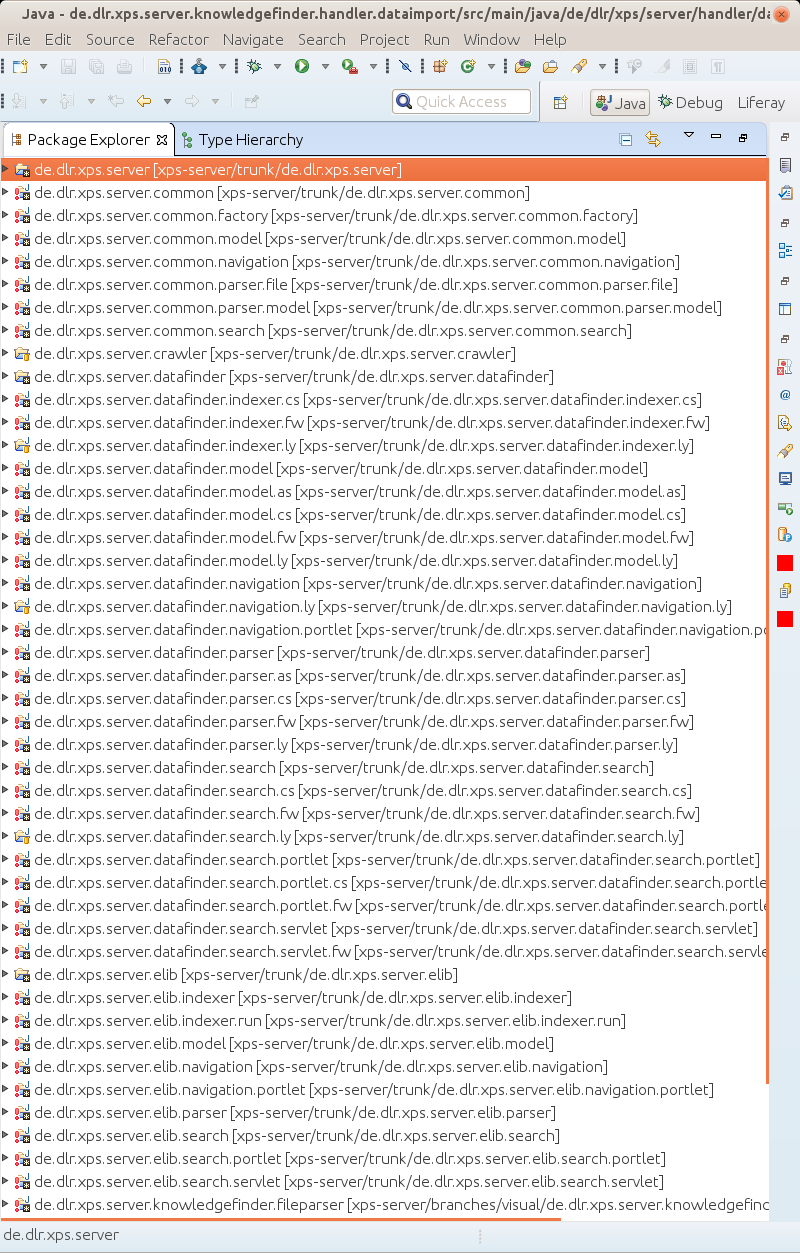
\includegraphics[width=0.7\textwidth]{eclipse.png}
  \caption{Las instancias del proyecto \gls{kf} en \gls{eclipse}}
  \label{image:eclipsekf}
\end{figure}

\sitem{La interfaz de usuario y la comunicación con el servidor}
Como se ha comentado en el apartado anterior, la interfaz de usuario está implementada usando una versión no actual de \gls{vaadin}, sin soporte técnico desde mayo de 2014. En el código del \gls{kf} es confuso, complejo y no se encuentra bien estructurado el sistema de tal forma que dentro del mismo proyecto no se puede diferenciar claramente entre los módulos, por ejemplo, de la interfaz de usuario y la importación de los datos.\\

Esta complejidad hace también que el mantenimiento y adaptación de la interfaz de usuario sea más tediosa y laboriosa.\\

En lo que respecta al tipo de tecnología, el \gls{framework} \gls{vaadin} necesita una constante comunicación con el servidor provocando que por cada interacción con el sistema el usuario tiene que esperar una respuesta del servidor.\\

El sistema de búsqueda de \gls{kf} está centrado y limitado al texto, tanto el sistema de búsqueda como la representación de los datos. A pesar de que los relación datos presentan una más compleja, estas relaciones no se muestran de forma directa. En la imagen \ref{image:monitor} se puede apreciar los distintos componentes de la interfaz para \gls{monitor}.

\begin{figure}[h!]
  \centering
    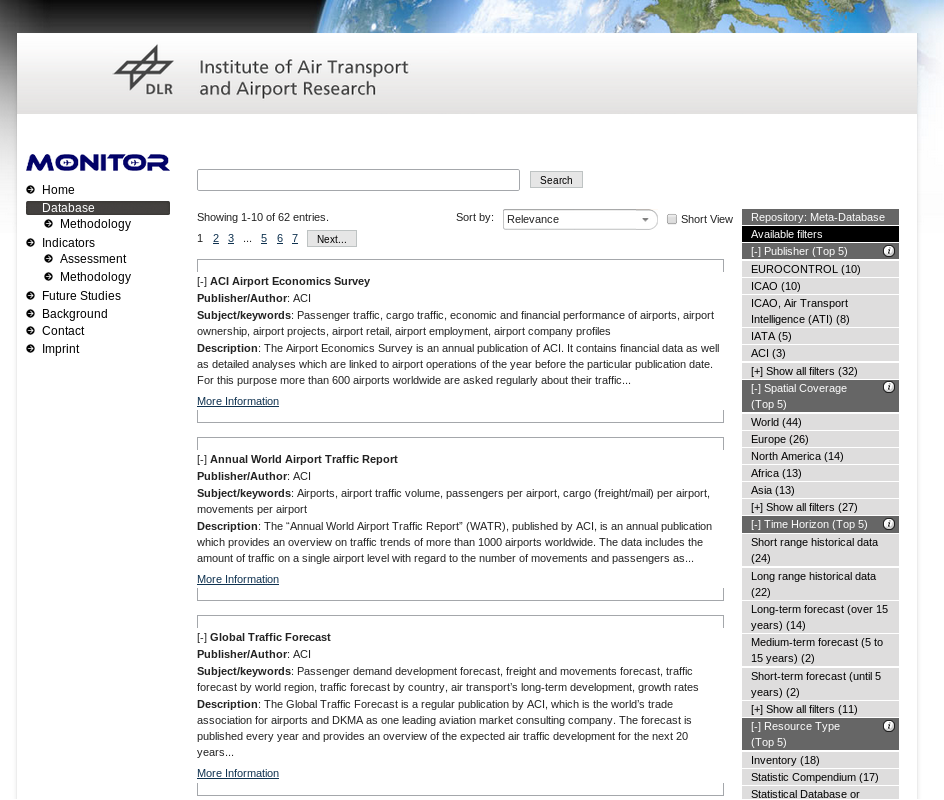
\includegraphics[width=0.8\textwidth]{monitor.png}
  \caption{Interfaz de usuario para \gls{monitor}}
  \label{image:monitor}
\end{figure}
\end{itemize}


% vaadin, lento pero en Java todo. nuevos componentes de UI muy complejo de crear si no existen en vaadin, combinar JS con JAVA usando GTW.


\section{\IfLanguageName{english}{Business Needs}{Necesidades de Negocio}}
%Esta sección debe contener información sobre los objetivos de negocio de clientes y usuarios, incluyendo los modelos de procesos de negocio a implantar.

A continuación se exponen los objetivos de negocio de clientes y usuarios, junto a los modelos de proceso de negocio, del proyecto \gls{kf2}
 
\subsection{\IfLanguageName{english}{Business Goals}{Objetivos de Negocio}}
Los objetivos de negocio de \gls{kf2} son:
\begin{itemize}
	\sitem{Simplificar adaptación del \gls{framework} para las distintas instancias}
    El nuevo \gls{kf2} tiene que ser un sistema que se adapte fácilmente a los distintos sistemas de conocimiento. Tanto el sistema de importación como la representación para el usuario debe ser fácilmente configurable y extensible.
    
    \sitem{Visualización gráfica del conocimiento}
	Para esta nueva versión del \gls{framework} se debe obtener una visualización gráfica del conocimiento que represente las relaciones y las estructuras complejas que existen los distintos \glspl{metadato}. A través de esta visualización el usuario deberá obtener una visión conjunta estas estructuras facilitando de esta forma la búsqueda de documentos. 
\end{itemize}
% \question{no es lo mismo que alcance de la sección de introducción \ref{chapter:introduccion}}
% Esta sección debe contener los objetivos de negocio que se esperan alcanzar cuando el sistema software a desarrollar esté en producción.

\subsection{\IfLanguageName{english}{Business Process}{Procesos de Negocio}}
% Esta sección, debe contener los modelos de procesos de negocio a implantar, que normalmente son los modelos de procesos de negocio actuales con ciertas mejoras.

En esta sección se exponen los procesos de negocio del \gls{framework} \gls{kf2}.

\subsubsection{Importación de los datos}
En este proceso de negocio se produce la importación de los datos provenientes de repositorios de \gls{svn} configurados. En la imagen \ref{image:negimport2} se representa el modelo proceso de este negocio en \gls{uml}.

\begin{figure}[H]
  \centering
    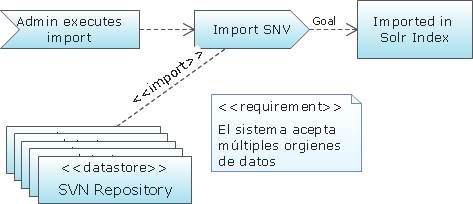
\includegraphics[width=0.8\textwidth]{NegocioNuevoImport.png} 
  \caption{Modelo de proceso de negocio, importación de los datos en \gls{kf2}}
  \label{image:negimport2}
\end{figure}

\subsubsection{Búsqueda en el portal}
Este proceso de negocio se produce cuando el usuario filtra el conjunto de documentos usando para ello la interfaz web. Como resultado de esta acción, el usuario obtiene una lista acorde con el filtro aplicado y una visualización de los documentos.  En la imagen \ref{image:negsearch2} se representa el modelo proceso de este negocio en \gls{uml}.

\begin{figure}[H]
  \centering
    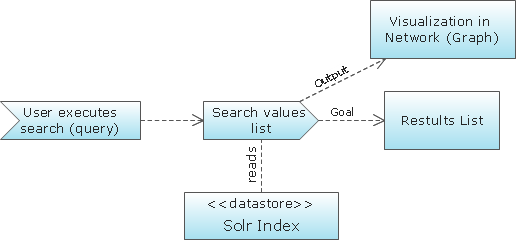
\includegraphics[width=0.8\textwidth]{NegocioNuevoSearch.png} 
  \caption{Modelo de proceso de negocio, búsqueda en el portal \gls{kf2}}
  \label{image:negsearch2}
\end{figure}

\section{Obtención de los Objetivos del Sistema}
Una vez extraídas las nuevas necesidades de negocio, era necesario refinarlos para obtener los objetivos reales del sistema. El punto más dificultoso fue la elección del elemento de visualización a diseñar. Para obtener más detalles sobre qué aspectos eran más importantes, se realizó un sondeo entre los institutos involucrados.\\

Las visualizaciones que más se acercaban a las necesidades concretas fueron:
\begin{itemize}
	\item \textbf{Chord Diagram} (imagen \ref{image:corddiagram})
    \begin{figure}[H]
      \centering
    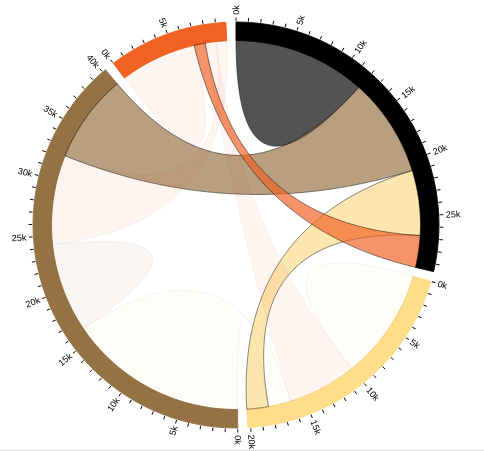
\includegraphics[height=0.35\textheight]{chord.png}
      \caption{Chord Diagram}
      \label{image:corddiagram}
    \end{figure}
    
   	\item \textbf{Bubble Chart} (imagen \ref{image:bubble})
     \begin{figure}[H]
      \centering
    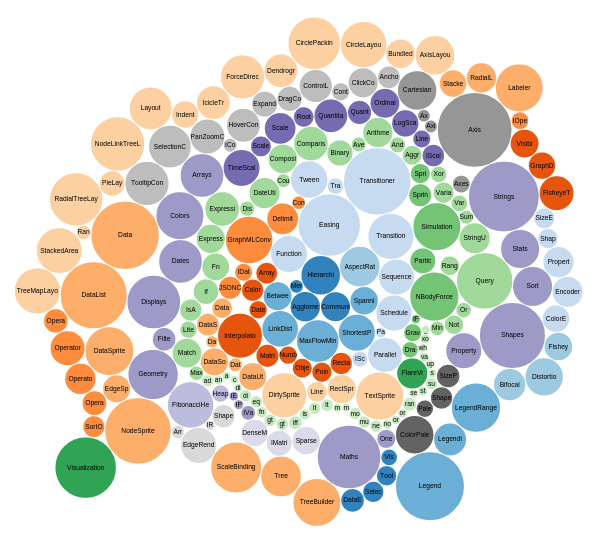
\includegraphics[height=0.35\textheight]{bubble.png}
      \caption{Bubble Chart}
      \label{image:bubble}
    \end{figure}

	\item \textbf{Circle Packing} (imagen \ref{image:packing})
     \begin{figure}[H]
      \centering
    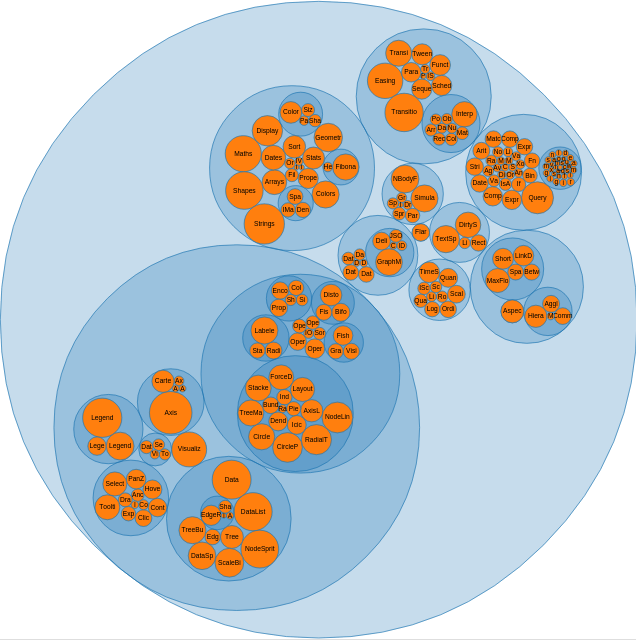
\includegraphics[height=0.35\textheight]{circle.png}
      \caption{Circle Packing}
      \label{image:packing}
    \end{figure}
	\item \textbf{Grafo - Force Layout} (imagen \ref{image:graphlayout})
     \begin{figure}[H]
      \centering
    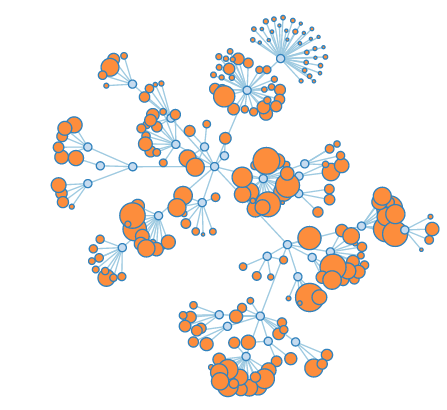
\includegraphics[height=0.35\textheight]{layout.png}
      \caption{Grafo - Force Layout}
      \label{image:graphlayout}
    \end{figure}
\end{itemize}

Tras varias conversaciones para saber qué propiedades eran las más interesantes de cada uno, se optó por el grafo de \glspl{metadato} como elemento central de la visualización para el proyecto ya que sus relaciones representan las estructuras complejas con más fidelidad y es más intuitivo para el usuario.

\section{\IfLanguageName{english}{System Goals}{Objetivos del Sistema}}
% \question{Objetivos del sistema? objetivos del negocio? que poner aqui??}Esta sección debe contener la especificación de los objetivos o requisitos generales del sistema.

% \question{Qué pasa con la obtención de requisitos, donde puedo incluir las entrevistas y ese proceso?}

\subsection{Importación y adaptación configurable}
El sistema de importación e indexación debe aceptar nuevos repositorios \gls{svn}. A su vez, el sistema encargado de la \gls{ui} debe ser igualmente configurable y extensible a través de ficheros de configuración para adaptarse las peculiaridades de cada portal.

\subsection{Representación de los \glspl{metadato} en un grafo}
Los \glspl{metadato} extraídos durante el proceso de indexación se deben mostrar en un grafo interactivo junto con sus relaciones. A través de este grafo, el usuario podrá definir sus criterios de búsquedas.


\section{\IfLanguageName{english}{System Requirements}{Catálogo de Requisitos}}
%Esta sección debe contener la descripción del conjunto de requisitos específicos del sistema a desarrollar para satisfacer las necesidades de negocio del cliente.
A continuación, en este apartado se describen los requisitos del proyecto \gls{kf2}.

\subsection{Requisitos de interfaces externas}

A continuación se describirán los requisitos de conexión con otros sistemas de software con los que el sistema va a interactuar para la importación de los \glspl{metadato} así como la \gls{ui}.

\subsubsection{Importación de los datos externos}
La importación de la información del portal se realizará partiendo de uno o varios repositorios de \gls{svn}. Estos repositorios podrán ser remotos, necesitando en su caso autenticación, o una copia de trabajo local. La información de los valores a importar se encontrará en las propiedades de \gls{svn} en formato \gls{json}.


\subsubsection{\Gls{ui}}
La \gls{ui} se usará por los usuarios para consultar con los datos indexados en el momento de la importación a través de un navegador web.\\

Los requisitos de la \gls{ui} del \gls{kf2} la podemos descomponer en los siguientes elementos; menú, grafo de exploración, selección actual, campo \gls{fulltext} y la lista de resultados.


\sparagraph{Menú}
Para una navegación clásica, el usuario dispondrá de un menú interactivo de navegación para gestionar los filtros que se desean aplicar a la búsqueda. Para este menú se requiere las siguientes características:

\begin{itemize}
\sitem{Multinivel}
El menú constará como máximo de dos subniveles de navegación y como mínimo uno.

\sitem{\Gls{scroll} en las opciones de menú}
Para las listar largas de opciones en el menú, éste debe de disponer de un \gls{scroll}.

\sitem{Contador de documentos por filtro en el menú}
En menú se dispondrán de un contador por cada filtro aplicable con el número de documentos que actualmente contienen el correspondiente filtro. 

\sitem{(Re)ordenación del menú}
Las opciones del menú obtenidas deben mantener el siguiente orden; primero las opciones seleccionadas y luego el resto de opciones ordenadas por el número que indique su contador de documentos correspondiente. 

\sitem{Grupos en acordeón}
La lista de elementos de un submenú deberán mostrarse dentro de un sistema de acordeón.
\end{itemize}

\subsubsection{Grafo de exploración}
Los \glspl{metadato} del conjunto de elementos importados deberán representarse en un grafo interactivo que muestre las relaciones entre ellos y la relevancia de éstos dentro del conocimiento en su totalidad.

\subsubsection{Selección actual}
En la interfaz de usuario se deben mostrar en una lista con los filtros actualmente han sido activados.

\subsubsection{Campo \gls{fulltext}}
La \glslink{ui}{interfaz} hará posible que el usuario pueda introducir texto libremente para que sea usado en el sistema de búsqueda.

\subsubsection{Lista de resultados}
Los documentos resultado de la búsqueda deberán de ser mostrados en una lista. En esta lista se deben poder diferenciar claramente los distintos elementos que la componen. También deberá cumplir las siguientes propiedades: 

\begin{itemize}
\sitem{Lista de resultados en forma de acordeón}
La lista de resultados debe mostrar el título de cada uno de los documentos y la posibilidad de una pequeña visualización de resumen de algunos campos seleccionados usándose un sistema de acordeón.

\sitem{\Gls{paginacion} en los resultados}
Para un gran número de resultados, la lista debe ser mostrada usando una \gls{paginacion}.

\sitem{Ordenación en los resultados}
La lista de resultados deberá ser mostrada en un orden seleccionable por el usuario.

\sitem{Detalles de los documentos}
En sistema debe permitir seleccionar un documento de la lista de resultados y mostrar todos sus campos disponibles en una ventana emergente.

\sitem{Contador de elementos en lista}
Como parte de la interfaz, el usuario dispondrá de manera clara de un contador con el número total de documentos para estado actual de la búsqueda. 
\end{itemize}


\subsection{\IfLanguageName{english}{Functional Requirements}{Requisitos funcionales}}
\label{subsection:funcionales}
%Descripción completa de la funcionalidad que ofrece el sistema.

\sparagraph{Pliegue y despliegue de la lista de resultados}
La interfaz de usuario debe permitir el pliegue y despliegue de cada elemento de la lista de resultados o todos con una simple acción.

\sparagraph{Pliegue y despliegue del menú}
La interfaz de usuario debe permitir el pliegue y despliegue de los elementos de menú con subgrupos. El usuario podrá desplegar o contraer los subelementos por cada grupo del menú.

% funcional
\sparagraph{Aplicar filtro de \gls{metadato}}
Cuando el usuario pulse sobre un \gls{metadato} (en grafo de exploración o en el menú) se debe filtrar los resultados acorde con el \gls{metadato} seleccionado. Si pulsa una arista que comunica dos \glspl{metadato}, se aplicara el filtro de ambos.

% funcional
\sparagraph{Desactivar filtro de \gls{metadato}}
Cuando el usuario pulse sobre un \gls{metadato} en el menú que ya esté aplicado o sobre la lista de la actual selección, éste se desactivará. 

% funcional
\sparagraph{Texto informativo de \gls{metadato}}
Cuando el usuario se encuentre sobre un \gls{metadato} (en gráfica de visualización o en el menú) se debe mostrar un texto con información adicional sobre éste.

\sparagraph{Resaltado de \gls{metadato}}
Cuando el usuario se encuentre sobre un \gls{metadato} (en gráfica de visualización o en el menú) se deben resaltar los elementos relacionados en el grafo, el correspondiente en el menú y los documentos que contienen ese \gls{metadato}.

\sparagraph{Resaltado de los \glspl{metadato} de documentos}
Cuando el usuario se sitúe sobre un documento de la lista de resultados se deben resaltar los \glspl{metadato} y las relaciones entre ellos en el grafo y en el menú.

% funcional?
\sparagraph{Búsqueda en el \gls{fulltext}}
El usuario a través del campo de búsqueda \gls{fulltext} podrá realizar búsquedas aproximadas, combinadas con operadores disyuntivos o conjuntivos, búsqueda exacta de texto y expresiones regulares simples (!, ?, *, \dots).\\

% funcional?
\sparagraph{Detalles de los documentos}
En sistema debe permitir seleccionar un documento de la lista de resultados y mostrar todos sus campos disponibles, dependiendo de los roles del usuario, en una ventana emergente.  

% funcional
\sparagraph{Interacción del menú con el gráfico visual}
Desde el menú, el usuario podrá activar o desactivar los grupos de \glspl{metadato} se mostrarán en el gráfico.

\subsection{\IfLanguageName{english}{Not-functional Requirements}{Requisitos no funcionales}}
%Descripción de otros requisitos (relacionados con la calidad del software) que el sistema deberá satisfacer: portabilidad, seguridad, estándares de obligado cumplimiento, accesibilidad, usabilidad, etc.

%%%%%%%%%%%%%%%%%%%%
% no funcional
\sparagraph{Adaptación de los campos sistema de importación }
El sistema de importación de los datos debe ser fácilmente configurable para añadir o suprimir campos en el índice de búsqueda. 

\sparagraph{Adaptación del sistema de importación}
La incorporación de nuevos tipos de fuentes de datos (por ejemplo desde ficheros \gls{xml}) tiene que ser relativamente simple.

\sparagraph{Adaptable a los roles del usuario}
El sistema debe permitir la configuración y combinación de roles para personalizar el resultado de las consultas y los campos a mostrar.

% no funcional
\sparagraph{Compartición del estado del portal usando \gls{url}}
Partiendo del supuesto de que tienen los mismos permisos, los usuarios podrán compartir el estado de la búsqueda y de la visualización a través de la dirección \gls{url} generada.

% no funcional
\sparagraph{Comportamiento dinámico del elemento visual}
El elemento visual debe comportarse de forma dinámica, es decir, que por cada cambio que deba producirse en él no se deba redibujar todo el gráfico, sólo las partes implicadas.

\sparagraph{Interacción de los componentes}
Los componentes de la \gls{ui} deben interaccionar entre ellos en la medida de lo posible tal que el usuario no perciba un descenso del rendimiento de la aplicación.

% no funcional
\sparagraph{Tiempo de respuesta de la interfaz}
Tanto la visualización como la búsqueda tendrá tiempo de respuestas aceptables a las peticiones de un usuario con un sistema y conexión estándar. El usuario debe poder interaccionar con el sistema sin percibir la comunicación con el servidor.

% no funcinal
\sparagraph{Ampliable con futuros elementos gráficos}
En un futuro debe ser posible la fácil incorporación de nuevos elementos gráficos a la \gls{ui}. La inclusión de mapas y lineas de tiempo que interactúen con el resto de componentes debe ser simple y eficiente.

% no funcional
\sparagraph{Grafo debe ser fácilmente configurable}
Aspectos como la complejidad o el estilo del gráfico interactivo deben ser fácilmente configurable.

\sparagraph{Lista de resultados debe ser fácilmente configurable}
Aspectos como la paginación o las opciones de ordenación deben 
ser fácilmente configurables.

% no funcional
\sparagraph{El menú debe ser fácilmente configurable}
El menú con las opciones de filtrado debe ser configurable hasta dos niveles (orden, estilos, textos, subelementos, \gls{scroll}, desplegado, \dots).

\sparagraph{Actualización automática del menú}
En su último nivel, las opciones son obtenidas de forma automática en el momento de la primera carga de la página.

% no funcional
\sparagraph{El estado inicial del gráfico fácilmente configurable}
El gráfico de visualización por defecto mostrado en la visita inicial de la aplicación debe ser configurable con relativa simpleza.

%  no funcional
\sparagraph{Carga en paralelo de los componentes}
Los componentes que forman el \gls{ui} deben de generarse y actualizarse en paralelo dentro de las posibilidades de las tecnologías de visualización y del navegador que el usuario esté usando.

\sparagraph{Estilos configurables}
Los estilos de los componentes que forman la \gls{ui} deben de ser fácilmente configurables conjuntamente.

\subsection{\IfLanguageName{english}{Engine Rules}{Reglas de negocio}}
% En el desarrollo del sistema, hay que tener en cuenta las denominadas reglas de negocio, es decir, el conjunto de restricciones, normas o políticas de la organización que deben ser respetadas por el sistema, las cuales suelen ser cambiantes.
\sparagraph{\Gls{java}, el lenguaje de programación}
Dado el carácter piloto de \gls{kf2}, el proyecto debe ser desarrollado en la medida de lo posible en un lenguaje dominado por el personal del \gls{scvss}. En este caso \gls{java} debe de ser usado como lenguaje de programación para el sistema de indexación
 
\subsection{\IfLanguageName{english}{Information Requirements}{Requisitos de información}}
% En esta sección se describen los requisitos de gestión de información (datos) que el sistema debe gestionar.



El sistema de información de \gls{kf2} está basado en un índice de búsqueda \gls{nosql}. Se mantendrá el mismo esquema expuesto en la imagen \ref{image:stradadata} exceptuando los campos que representan intervalos de tiempo, por ejemplo ``Temporal Coverage''.  Estos campos del índice proporcionarán la fecha máxima y mínima para los valores posibles dados para simplificar posibles consultas usando fechas. En la tabla \ref{table:transformtab} se representa algunas transformaciones posibles.

\begin{center}
	\begin {table}[H]
	\centering
      \begin{tabular}{| c | c | c|}
      \hline
      \textbf{Valor} & \textbf{Fecha mín.} & \textbf{Fecha máx.}\\ \hline
      2003 - 2010 & 2003-01-01 & 2010-12-31 \\ \hline
          - 2010 			& NULL				& 2010-12-31   	\\ \hline
      2003 - 			& 2003-01-01 				& NULL  	\\ \hline
      2003-03 - 2010-11 			& 2003-03-01 				& 2010-11-31   	\\ \hline
      2003-03-10 - 2010-10-31 			& 2003-03-10 				& 2010-10-31   	\\ \hline
      \end{tabular}
    \caption{Tabla resumen de las transformaciones para los rangos de fechas}
    \label{table:transformtab}
  \end{table}
\end{center}

\subsection{Restricciones técnicas del sistema}

\sparagraph{\Gls{portlet} de \gls{liferay}}
La página web usada como interfaz de usuario debe ser un \gls{portlet} compatible con una versión actual de \gls{liferay}.

\sparagraph{Compatibilidad con \gls{html5}}
La aplicación debe ser compatible con \gls{html5} es decir con la amplia mayoría de los navegadores actuales. Por supuesto, el uso de la tecnología \gls{flash} no está permitido.



\section{Alternativas de Solución} 

%En esta sección, se debe ofrecer un estudio del arte de las diferentes alternativas tecnológicas que permitan satisfacer los requerimientos del sistema, para luego seleccionar (si procede) la herramienta o conjunto de herramientas que utilizaremos como base para el software a desarrollar.
\begin{comment}

Frontend: Vaadin, GTK, buscar otros, creando un nuevo elemento, muy complejo crear adaptar el comportamiento de los existentes
Backend: adaptar el anterior sistema de importación mejorar rendimiento de las consultas...

usando MVN Excpliarlo 
Frontend nuevo componente JS, con los frameworks ...Cytoscape, sigma.js cargar grafo desde Neo4j o RDF crear imagen Canvas, 
Backend o importancion, adaptar el anterior y crear un servicio web
rediseñarlo usando solr para mejorar la importacion 

Seguridad
control de acceso de los usuarios
MoltMT de solr security
Crear un servico web con filtro de usuarios

estilos:
CSS directamente o SASS

otras cosas:
crossfilter timeline zoom, futuras mejoras...
\end{comment}

A continación se expone el estudio de la solución propuesta para el \gls{framework} \gls{kf2}.

\subsection{Elección de la tecnología de visualización}
Para la visualización del grafo descrito anteriormente, es necesario usar tecnología \gls{js}. Entre las posibles soluciones destacan:

\subsubsection{\gls{sigma}}
Sigma es una biblioteca \gls{opensource} de \gls{js} pura dedicada exclusivamente al dibujo de grafos interactivos (dinámicos y estáticos)  en aplicaciones web. \\

Con una configuración por defecto, esta biblioteca permite la representación ajustado al contenedor del grafo en \gls{webgl} o, si el navegador web lo permite, en \gls{canvas}.\\

Gracias a su \gls{api} pública y adaptando la configuración, se puede conseguir fácilmente 
una personalización de cómo dibujar y de cómo interactúa el grafo. También permite que el desarrollador incluya su propia funcionalidad para la representación de los nodos y conexiones.\\

Entre las propiedades a destacar es su rendimiento para representar gráficos con un altísimo número de nodos, en la imagen \ref{image:sigma2} se puede observar la exploración de un gran grafo de una red social usando este \gls{software}. Por otra parte, en la imagen  \ref{image:sigma} se representa una captura de pantalla de un ejemplo más simple de \gls{sigma}.

\begin{figure}[h!]
  \centering
    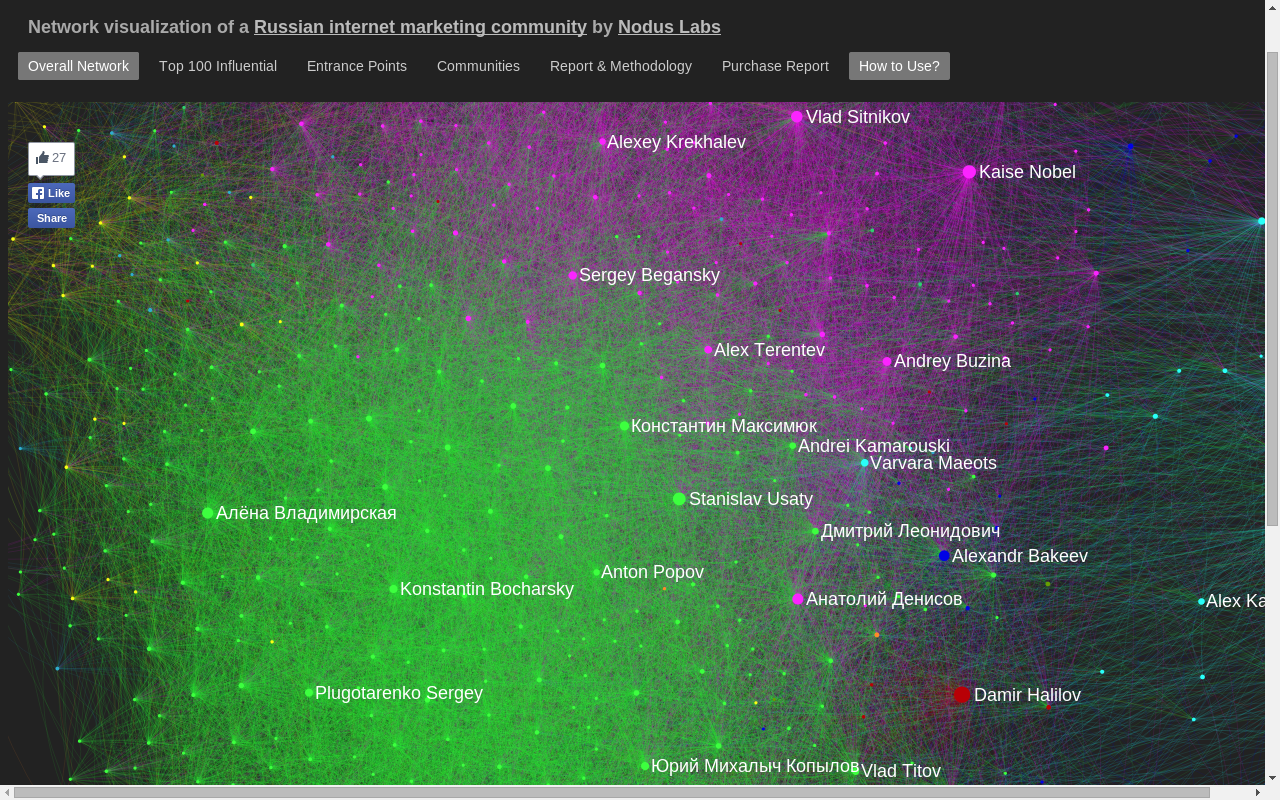
\includegraphics[width=0.8\textwidth]{sigma2.png}
  \caption{Exploración de una red social de marketing \gls{sigma} \cite{sigmaNodus}}
  \label{image:sigma2}
\end{figure}

\begin{figure}[h!]
  \centering
    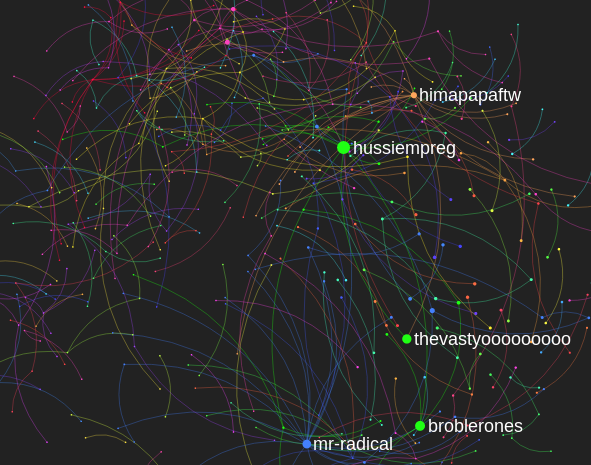
\includegraphics[width=0.7\textwidth]{sigmaTumblr.png}
  \caption{Exploración de la red de blogs Tumblr con  \gls{sigma} \cite{sigmaNodus}}
  \label{image:sigma}
\end{figure}

\subsubsection{\gls{cyto}}
\Gls{cyto} es una biblioteca \gls{opensource} escrita en \gls{js} para teoría de grafos, su visualización y análisis.\\

Permite la manipulación y representación de grafos interactivos facilitando al usuario crear sus propios eventos y personalizar la interacción con los grafos. Se integra con facilidad en las aplicaciones web y es compatible con los actuales navegadores.\\

En su biblioteca de funciones hay implementadas un conjunto de herramientas enfocadas a la teoría de grafos.\\

En la imagen \ref{image:cyto} podemos observar algunos ejemplos gráficos extraídos de su repositorio \cite{cyto}.

\begin{figure}[h!]
  \centering
    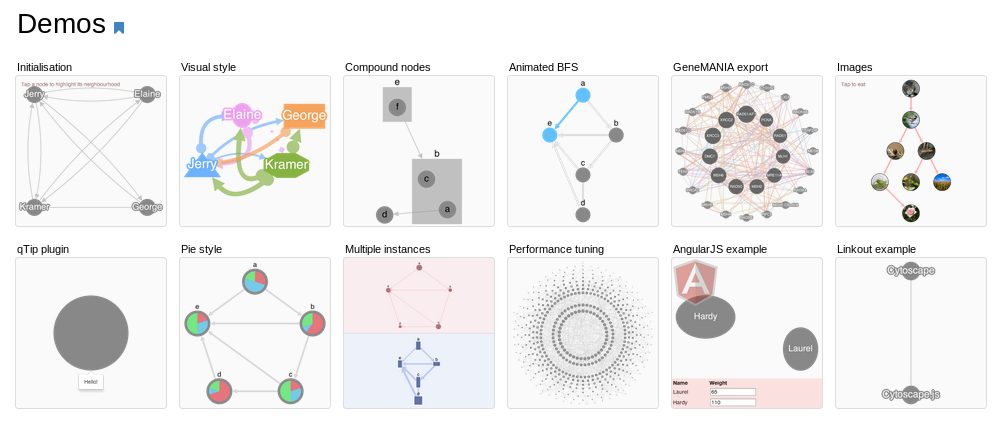
\includegraphics[width=0.9\textwidth]{cytoscape.png}
  \caption{Ejemplos visuales uso de \gls{cyto} \cite{cyto}}
  \label{image:cyto}
\end{figure}


\subsubsection{\gls{d3}}
\Gls{d3} es una biblioteca \gls{opensource} de \gls{js} para la manipulación de documentos basados en datos. Apoyándose en \gls{html5}, \gls{svg} y \gls{css} ayuda a mostrar a través de elementos visuales y manipular los datos de forma dinámica en aplicaciones web.\\

Una de sus bases es mantener los estándares facilitando  de esta forma que el \gls{software} desarrollado con él  sea compatible con los navegadores actuales.\\

La funcionalidad de \gls{d3} se basa en la conexión de la información con el \gls{dom} y la aplicación de transformaciones sobre el documento basado en unos en datos proporcionados. En el código \ref{code:d3data} podemos ver cómo de sencillo y simple se relacionan los datos con los componentes del \gls{dom}. En la imagen \ref{image:d3dataimage} el resultado interno de esta vinculación.\\


\begin{listing}
\begin{minted}[linenos,
               numbersep=5pt,
               frame=single,
               framesep=2mm]{javascript}
               
>>>> my_data = [20, 7, 32]
[20, 7, 32]
>>> d3.selectAll('.box').data(my_data).text( function(d) { return d } )
[[div.box, div.box, div.box]]

	\end{minted}
	\caption{Ejemplo de vinculación de datos con el \gls{dom} usando \gls{d3} \cite{D3exp2012}}
	\label{code:d3data}
\end{listing}

\begin{figure}[h!]
  \centering
    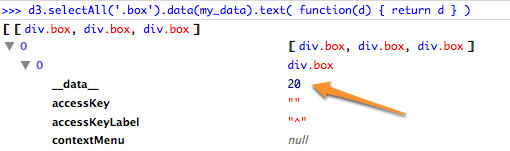
\includegraphics[width=0.7\textwidth]{domD3.png}
  \caption{Exploración del \gls{dom} después de la vinculación de datos \cite{D3exp2012}}
  \label{image:d3dataimage}
\end{figure}



Esta librería soluciona de forma eficiente la manipulación de documentos basados en datos y gracias a ello, permite que comportamientos dinámicos y de animación en los elementos visuales.\\

Todo esto junto con la claridad y calidad del código y la documentación de \gls{d3} facilita enormemente creación y reutilización de componentes visuales. Dentro de la biblioteca se encuentran ya definidos y extensamente documentados numerosos \glspl{plugin} visuales que ayudan para desarrollar nuestros propios elementos, adaptándose fácilmente a las necesidades de cada situación.\\

Uno de los puntos más fuertes de esta librería es su interacción entre los componentes y la facilidad de adaptación para usarse con otros sistemas. Por ejemplo, hacer funcionar \gls{d3} con la biblioteca para el uso de mapas \gls{leaflet} (imagen \ref{image:leaflet}) o con las gráficas de \gls{crossfilter} (imagen \ref{image:crossfilter}) es relativamente trivial.\\


\begin{figure}[h!]
  \centering
    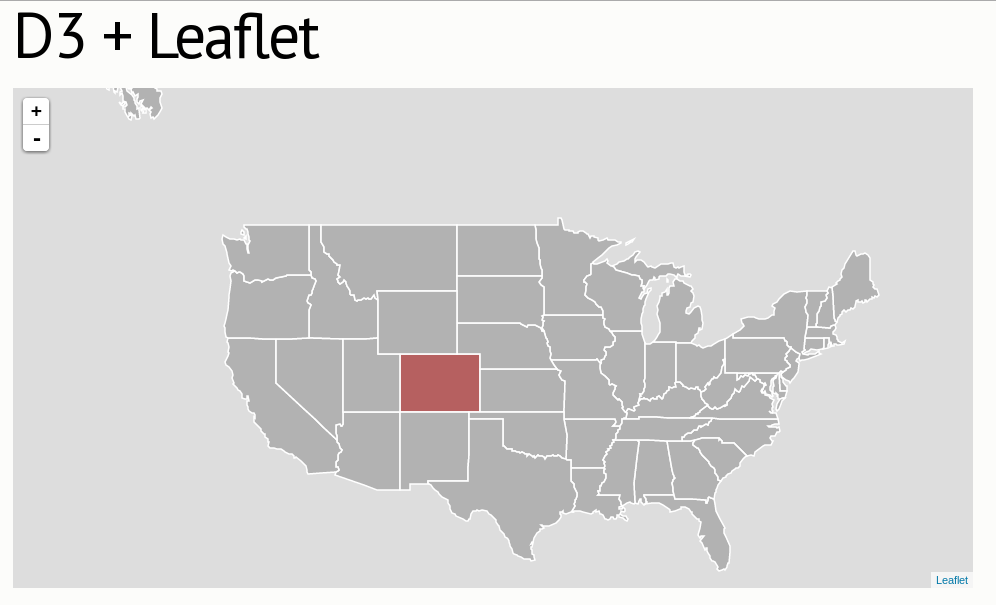
\includegraphics[width=0.8\textwidth]{leaflet.png}
  \caption{Ejemplo de integración de \gls{leaflet} con \gls{d3} usando mapas de GeoJSON \cite{d3leaflet}}
  \label{image:leaflet}
\end{figure}


\begin{figure}[h!]
  \centering
    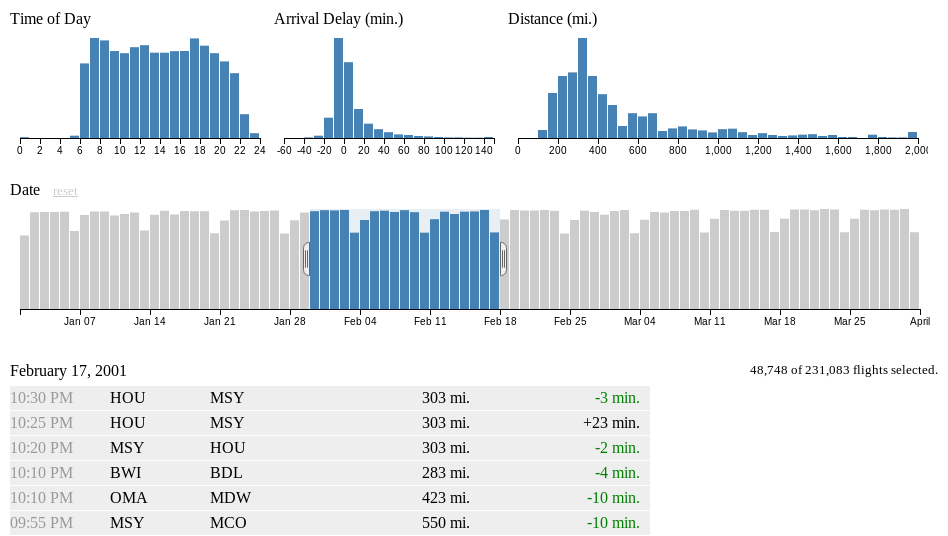
\includegraphics[width=0.8\textwidth]{crossfilter.png}
  \caption{Ejemplo de funcionamiento de \gls{crossfilter} \cite{crossfilter}}
  \label{image:crossfilter}
\end{figure}


Por otra parte, el gran número de ejemplos públicos desarrollado por terceros publicados bajo un mismo patrón bajo la dirección \url{http://bl.ocks.org/} hace que éstos puedan visualizarse directamente en la web y junto respaldado por una muy activa comunidad hacen que la labor del desarrollador sea productiva y eficaz. En la figura \ref{image:D3force} podemos observar uno de estos ejemplos aplicado a grafos.

\begin{figure}[h!]
  \centering
    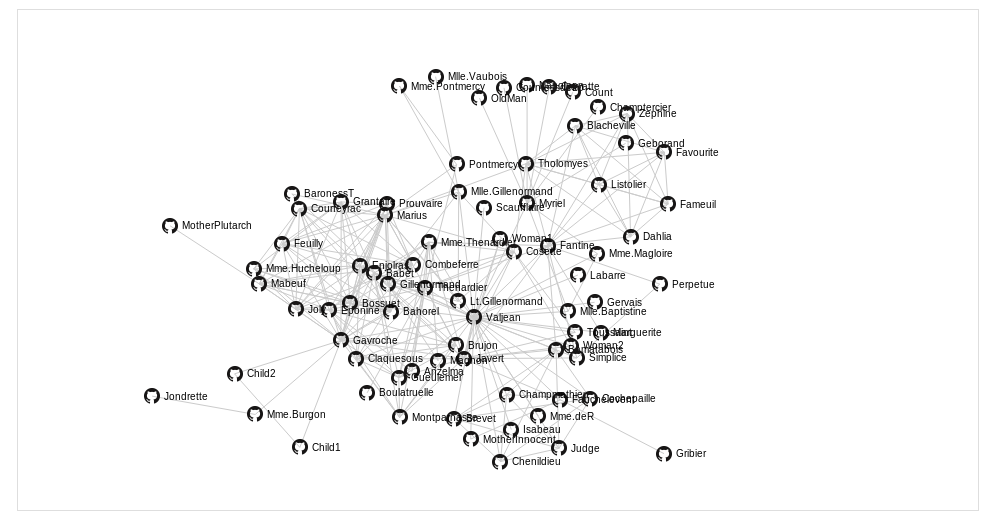
\includegraphics[width=0.8\textwidth]{D3force.png}
  \caption{Ejemplo de grafo en \gls{d3} publicado en \url{http://bl.ocks.org/mbostock/950642}}
  \label{image:D3force}
\end{figure}

\Gls{d3} trabaja sobre \gls{svg} por defecto para sus librerías gráficas. Esto tiene el inconveniente de que elementos visuales muy complejos tiene un bajo rendimiento.

\subsection{Elección del índice de búsqueda}
Para el proyecto \gls{kf} utilizó un índice de búsqueda \gls{lucene} en su versión 3.0.2. Dadas las restricciones provenientes de \gls{scvss} el índice de búsqueda del proyecto \gls{kf2} deberá basarse en éste.\\

Por este motivo, la única posible elección es la utilización, sobre una instancia de \gls{lucene}, de la plataforma de búsqueda \gls{solr} o directamente el propio \gls{lucene}.\\ 

\Gls{solr} amplia el potencial de \gls{lucene} mejorando principalmente las siguientes funcionalidades:

\begin{itemize}
	\item Opciones más potentes para \gls{fulltext}.
    \item Optimizado para gran volumen de tráfico web.
    \item Interfaces estandarizadas de \gls{xml}, \gls{json} y \gls{http}.
    \item Panel intuitivo de administración.
    \item Estadísticas del servidor para monitorización en \gls{jmx}.
    \item Escalable linealmente, replicación automática, tolerancia a fallos y restauración automática \cite{solroncloud}.
    \item Cercano a la indexación en tiempo real.
    \item Flexible y fácilmente adaptable usando configuración en formato \gls{xml}.
    \item Arquitectura ampliable de \glspl{plugin}.
\end{itemize}

\subsection{Elección del tipo de aplicación}
Las dos opciones planteadas como posibles tipos de aplicación dependiendo el tipo de arquitectura a implantar.

\subsubsection{Aplicación Enriquecida de Internet (\gls{ria})}
Como se explicó en la sección \ref{subsection:entornotech} el \gls{framework} \gls{kf} utiliza para su desarrollo una arquitectura \gls{ria} usando los componentes de \gls{vaadin} 6.8.14 .\\

Para poder representar los elementos gráficos anteriormente descritos, es necesario la actualización a la versión actual de \gls{vaadin} y el desarrollo de los nuevos componentes y de esta forma adaptarlos al modelo arquitectónico definido por \gls{ria}.\\

En este modelo en el cliente, el navegador web, no se realiza cálculos. Estos son diferidos a través de \gls{ajax} al servidor que es el encargado de toda la lógica de la aplicación. Esto conlleva a que la mayoría de las interacciones del usuario con la aplicación necesite una consulta al servidor web.

\subsubsection{Modelo Vista Controlador (\glslink{mvc}{MVC})}
\label{subsubsection:mvc}
Este planteamiento de arquitectura web dista del planteado en el proyecto predecesor \gls{kf}. Se basa en separar en tres partes la aplicación:

\begin{itemize}
	\sitem{El Modelo}
    Representa la información con la que el sistema trabaja. En el caso de \gls{kf2} sería principalmente el índice de búsqueda. 
    
    \sitem{El Controlador}
    Responde a los eventos invocados desde la vista por, normalmente, el usuario e invoca las peticiones al modelo. En nuestro caso sería un servicio web que serviría de intermediario entre la la vista y el índice de búsqueda. Este servicio web estaría integrado en el propio \gls{liferay} para definir su comportamiento dependiendo del usuario actual de la plataforma.
    
    \sitem{La Vista}
    Es la representación del modelo en un formato para interactuar, por ejemplo en una interfaz de usuario. Para el proyecto \gls{kf2} la vista representaría la página web donde se aloja la visualización y todos sus componentes.
\end{itemize}
 

\section{\IfLanguageName{english}{Proposed Solution}{Solución Propuesta}}
\begin{comment}
Si se ha optado por utilizar un software de base, debemos identificar y medir las diferencias entre lo que proporciona este software y los requisitos definidos para el proyecto.\\
El resultado de este análisis permitirá identificar cuáles de éstos requisitos ya están solventados total o parcialmente por el sistema base y cuales tendremos que diseñar e implementar la propuesta de solución.
\end{comment}

La elección del \gls{software} a emplear para la implementación de \gls{kf2} se trabajó muy estrechamente con \gls{fw} y \gls{vf}. Su feed-back fue decisivo para la toma de decisiones a nivel de usuario.\\

Respecto al desarrollo y el tipo de tecnología a desarrollar, el \gls{scvss} como futuro heredero del proyecto estimó que las soluciones planteadas fuesen compatibles con la motivación y erudición de los componentes del departamento.

\subsection{Elección de la tecnología de visualización}

El proceso de estudio comenzó con pruebas y demostraciones de las tecnologías disponibles para la visualización del conocimiento, el punto más influyente para  \gls{vf} y \gls{fw}. Cómo resultado de este estudio, realizado en la fase de ``Extended Static Prototype'' (apartado \ref{subsubsection:aplicandoextre}), se optó por la tecnología de \gls{d3}. Los puntos decisivos para esta decisión fueron:

\begin{itemize}
    \item Facilidad de personalizar el comportamiento de los componentes gracias a \gls{svg}.
    \item Calidad de la documentación y ejemplos ilustrativos de su uso.
    \item Compatibilidad entre los \glspl{plugin} actualmente definidos.
    \item Calidad del \gls{software}. 
    item  Facilidad de adaptación a las actuales y futuras necesidades específicas de \gls{kf2}.
\end{itemize}

\subsection{Elección del índice de búsqueda}

Tras un desacuerdo y una fuerte oposición inicial por parte del \gls{scvss} en cambiar el núcleo del sistema de indexación por motivos temporales y de costes adicionales,
se optó finalmente por la redefinición del sistema de importación e índice de búsqueda usando \gls{solr}. Como puntos claves de esta decisión fueron las siguientes propiedades de \gls{solr}:

\begin{itemize}
    \item Unificación de los proyectos \gls{lucene} y \gls{solr} en marzo de 2010.
    \item Sistema de configuración de \gls{solr} basado en ficheros \gls{xml}.
	\item Opciones más potentes para \gls{fulltext}.
    \item Optimizado para gran volumen de tráfico web.
    \item Múltiples clientes para el acceso a \gls{solr} con diferentes lenguajes de programación. Por ejemplo, \gls{solrj} proporciona una \gls{api} para \gls{java} que permite añadir, actualizar y consular el índice de \gls{solr}.
    \item Capacidad de crear clusters de servidores para una mejor tolerancia a fallos.
    \item Herramientas de monitorización.
\end{itemize}

\subsection{Elección del tipo de aplicación}

Durante la fase de ``Extreme Prototype'' (apartado \ref{subsubsection:aplicandoextre}) se demostró que con una \gls{api} de un servicio web relativamente simple se conseguía una visualización muy satisfactoria para el usuario.\\

Nuevamente, se encontró con un primer rechazo por parte del \gls{scvss} de cambiar el tipo de aplicación totalmente. Esto conllevaba a descartar totalmente \gls{vaadin} como herramienta, replanteamiento del \gls{framework} \gls{kf2} para los proyectos de próxima implantación (\gls{elib}, \gls{strada}, \dots) y la implementación partiendo desde cero del \gls{software}.\\

A pesar de ser un gran cambio respecto al pensamiento inicial de \gls{scvss} de cómo se desarrollaría \gls{kf2}, se optó por la implantación del \glslink{mvc}{Modelo Vista Controlador} con un servicio web en base a los siguientes argumentos:

\begin{itemize}
    \sitem{Costosa y necesaria actualización de \gls{vaadin}}
    La versión de \gls{vaadin} usada para el proyecto \gls{kf} se encuentra desactualizada y sin mantenimiento. Para un correcto y eficiente funcionamiento con los sistemas complejos de visualización la nueva \gls{api} de \gls{js} de \gls{vaadin} 7 sería necesaria.

	\sitem {Difícil incorporación de los elementos  de \gls{d3} en \gls{vaadin}}
    Incluso la nueva versión del \gls{framework} \gls{vaadin} no proporciona ningún componente gráfico útil para la visualización de \gls{kf2}. Aún existiendo algunos proyectos inacabados como gwt-d3 \cite{gwtd3}, la integración de los componentes de \gls{d3} sería demasiado costosa.
    
    \sitem {Incierto rendimiento adecuado de la aplicación usando \gls{ria}}
    Con \gls{d3} se producen su alto número de peticiones al servidor. Con una arquitectura \gls{ria} esto se traduciría en una posible saturación de la parte del servidor y una lenta reacción de la interfaz de usuario.
    
    \sitem {Flexibilidad de \gls{mvc}}
    El patrón \gls{mvc} se basa en las ideas de reutilización de código y la separación de la aplicación (modelo, vista, controlador) para un fácil desarrollo y mantenimiento. En el caso de \gls{kf2}, esta arquitectura hace además que la adaptación y ampliación del \gls{framework} sea más sencilla y elegante.
    
    \sitem {\gls{d3} y los recursos externos}
    La \gls{api} de \gls{d3} facilita el uso de éste con servicios web en múltiples formatos (\gls{json}, \gls{xml}, fichero de texto, \dots) a través de llamadas por \gls{ajax}.
    
    \sitem {\gls{liferay} y los servicios web}
    El impuesto portal \gls{liferay} proporciona una interfaz de comunicación por \glspl{sw}. Esto hace que la implementación nuevos servicios para \gls{kf2} sea relativamente sencilla \cite{liferayws}. Para una comunicación de los componentes  \gls{js} a través de \gls{ajax} es una herramienta muy útil.
\end{itemize}


























\chapter{\IfLanguageName{english}{Systems analysis}{Análisis del Sistema}}
% ------------------------------------------------------------------------------
% Este fichero es parte de la plantilla LaTeX para la realización de Proyectos
% Final de Grado, protegido bajo los términos de la licencia GFDL.
% Para más información, la licencia completa viene incluida en el
% fichero fdl-1.3.tex

% Copyright (C) 2012 SPI-FM. Universidad de Cádiz
% ------------------------------------------------------------------------------

Esta sección cubre el análisis del sistema de información a desarrollar, haciendo uso del lenguaje de modelado \gls{uml}.

\section{\IfLanguageName{english}{Conceptual Model}{Modelo Conceptual}}
% \question{Cuál sería mi modelo conceptual?? no tengo ``un modelo de datos''}
% A partir de los requisitos de información, se desarrollará un diagrama conceptual de clases UML, identificando las clases, atributos, relaciones, restricciones adicionales y reglas de derivación necesarias.

En la imagen \ref{image:modeloconceptual} se muestra el diagrama conceptual para \gls{kf2}.

\begin{figure}[H]
  \centering
     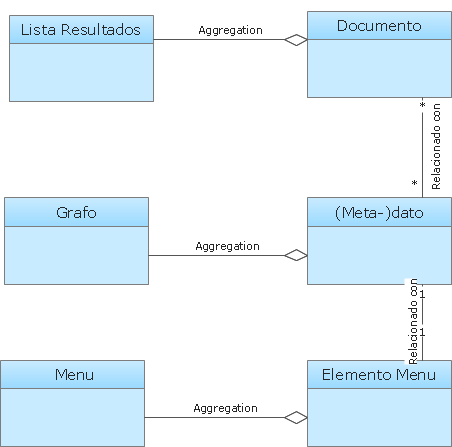
\includegraphics[width=0.7\textwidth]{Conceptual.png}
  \caption{Modelo Conceptual de \gls{kf2}}
  \label{image:modeloconceptual}
\end{figure}

\section{\IfLanguageName{english}{Use-case Model}{Modelo de Casos de Uso}}
% A partir de los requisitos funcionales descritos anteriormente, se emplearan los casos de uso como mecanismo para representar las interacciones entre los actores y el sistema bajo estudio. Para cada caso de uso deberá indicarse los actores implicados, las precondiciones y postcondiciones, los pasos que conforman el escenario principal y el conjunto de posibles escenarios alternativos.

Partiendo de los requisitos funcionales descritos en el apartado \ref{subsection:funcionales} se emplean los casos de uso para describir las interacciones de los actores y el \gls{kf2}.


\subsection{Diagramas de Casos de Uso}
En este apartado se va a describir algunos de los diagramas de caso de uso del proyecto. 

\subsection{\IfLanguageName{english}{Actors}{Actores}}
A continuación se exponen los diferentes roles que juegan los usuarios que interactúan con el sistema. Los actores pueden ser roles de personas físicas, sistemas externos o incluso el tiempo (eventos temporales).

\subsubsection{Administrador del índice de búsqueda}
Este actor será el encargado de controlar las importaciones de los datos en \gls{solr}. Puede ser una persona física que, a través de la interfaz de \gls{solr}, ejecute la importación o una tarea programada, por ejemplo un \gls{cron}.

\subsubsection{Usuario visitante}
\label{subsubsection:visitante}
Este actor utiliza la \gls{ui} sin estar registrado. No tiene autorización para iniciar sesión en el sistema. 

\subsubsection{Usuario registrado}
Este actor tiene permisos especiales concedidos por el \gls{dlr} para poder entrar en el sistema. Dependiendo de los permisos asignados, este actor dispondrá de un conjunto de documentos y campos extras. El sistema de acceso es externo al sistema.

\subsubsection{Diagrama Casos de Uso: Uso de la \gls{ui} (anónimo z registrado)}
En la imagen \ref{image:cuuiano} se representa los casos de uso para un usuario no registrado en el sistema (usuario visitante) y para uno registrado.

\begin{figure}[h!]
  \centering
     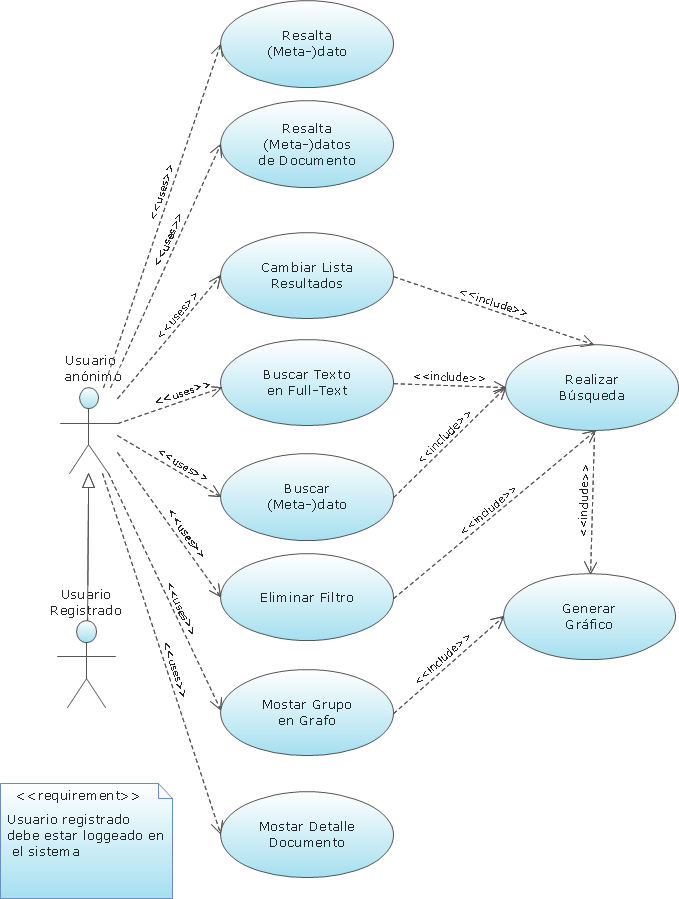
\includegraphics[width=0.8\textwidth]{UserCasesNormal.png}
  \caption{Diagrama Casos de Uso: Uso de la \gls{ui} (anónimo) y usuario registrado}
  \label{image:cuuiano}
\end{figure}

\begin{comment}
\subsubsection{Diagrama Casos de Uso: Uso de la \gls{ui}}
En la imagen \ref{image:cuuireg} se representa los casos de uso para un usuario registrado en el sistema.

\begin{figure}[h!]
  \centering
	\missingfigure{En libreta, Caso uso registrado}
  \caption{Diagrama Casos de Uso: Uso de la \gls{ui}}
  \label{image:cuuireg}
\end{figure}
\end{comment}
\subsubsection{Diagrama Casos de Uso: Gestión del índice de búsqueda}
En la imagen \ref{image:cuimport} se representa los casos de uso de un administrador del índice de búsqueda.

\begin{figure}[h!]
  \centering
     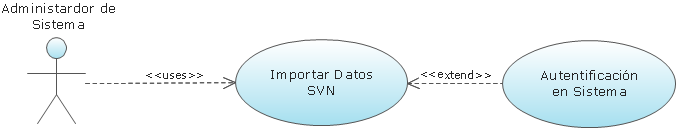
\includegraphics[width=0.8\textwidth]{UserCasesImport.png}
  \caption{Diagrama Casos de Uso: Gestión del índice de búsqueda}
  \label{image:cuimport}
\end{figure}

\subsection{Especificación de los Casos de Uso}

\subsubsection{Caso de Uso: Importación de datos}
\begin{itemize}
	\item{\textbf{Descripción}} El usuario activa la importación de los datos.
    \item{\textbf{Actor/es}} Usuario administrador del índice.
    \item{\textbf{Escenario Principal}}
    	\begin{enumerate}
        	\item El usuario selecciona una configuración a ejecutar.
			\item El usuario ejecuta importación con la configuración seleccionada.
            \item El sistema importa los documentos en el índice de búsqueda.
            \item El sistema muestra el resultado de la importación incluyendo los posibles errores.
        \end{enumerate}
\end{itemize}

\subsubsection{Caso de Uso: Buscar en \gls{fulltext}}
\begin{itemize}
	\item{\textbf{Descripción}} El usuario introduce un texto o expresión regular en el campo \gls{fulltext}.
    \item{\textbf{Actor/es}} Usuarios con o sin sesión iniciada.
    \item{\textbf{Escenario Principal}}
    	\begin{enumerate}
        	\item Usuario entra el texto a buscar en el campo \gls{fulltext}.
        	\item El sistema actualiza la lista de documentos únicamente con los elementos que contienen el texto introducido.
            \item El sistema actualiza el grafo de visualización con los nuevos valores de los \glspl{metadato} de los documentos encontrados (actualiza el tamaño de los nodos y de las relaciones entre ellos).
            \item El sistema actualiza los valores de los contadores en el menú.
            \item El sistema añade el valor introducido a la lista de filtros activos.
            \item El sistema sitúa la paginación en su primera página.
        \end{enumerate}
%    \sitem{Escenario Alternativo}
\end{itemize}



\subsubsection{Caso de Uso: Buscar \gls{metadato}}
\begin{itemize}
	\item{\textbf{Descripción}} El usuario filtra los documentos por un \gls{metadato} a través del grafo de visualización o del menú.
    \item{\textbf{Actor/es}} Usuarios con o sin sesión iniciada.
    \item{\textbf{Escenario Principal}}
    	\begin{enumerate}
        	\item Usuario pulsa sobre un nodo el nodo del grafo o sobre el elemento de la tabla que desea filtrar.
        	\item El sistema actualiza la lista de documentos suprimiendo aquellos que no contienen \gls{metadato} seleccionado.
            \item El sistema actualiza el grafo de visualización con los nuevos valores de los \glspl{metadato} de los documentos encontrados (actualiza el tamaño de los nodos y de las relaciones entre ellos).
            \item El sistema actualiza los valores de los contadores en el menú.
            \item El sistema añade el \gls{metadato} a la lista de filtros activos.
            \item El sistema sitúa la paginación en su primera página. 
        \end{enumerate}
    \item{\textbf{Escenario Alternativo}}
    	\begin{enumerate}[label=2.\alph*]
    		\item El \gls{metadato} seleccionado se muestra en el grafo.
            \begin{enumerate}[label=\arabic*]
            	\item El sistema elimina el elemento del grafo..
            	\item Continuar con el paso 3.
            \end{enumerate}
        \end{enumerate}
\end{itemize}

\subsubsection{Caso de Uso: Detalles de documento}
\begin{itemize}
	\item{\textbf{Descripción}} El usuario de \gls{ui} obtiene los detalles de un documento en una ventana emergente.
    \item{\textbf{Actor/es}} Usuarios con o sin sesión iniciada.
    \item{\textbf{Escenario Principal}}
    	\begin{enumerate}
        	\item Usuario selecciona un elemento de la lista de resultados.
        	\item El sistema despliega el acordeón del elemento.
            \item El usuario pulsa el botón para ver los detalles del documento.
            \item El sistema abre una ventana emergente donde muestra los campos permitidos para el usuario.
        \end{enumerate}
\end{itemize}

\subsubsection{Caso de Uso: Eliminar filtro}
\begin{itemize}
	\item{\textbf{Descripción}} El usuario de \gls{ui} elimina un filtro de los actuales activos en la lista filtros activos.
    \item{\textbf{Actor/es}} Usuarios con o sin sesión iniciada.
    \item{\textbf{Escenario Principal}}
    	\begin{enumerate}
        	\item Usuario selecciona un elemento de la lista formada por los filtros que con anterioridad fueron activados.
			\item El sistema actualiza la lista de documentos aplicando el resto de filtros que todavía siguen activos.
            \item El sistema actualiza el grafo de visualización con los nuevos valores de los \glspl{metadato} de los documentos encontrados (actualiza el tamaño de los nodos y de las relaciones entre ellos).
            \item El sistema actualiza los valores de los contadores en el menú.
            \item El sistema suprime el filtro la lista de filtros activos.
            \item El sistema sitúa la paginación en su primera página.
        \end{enumerate}
\end{itemize}


\subsubsection{Caso de Uso: Cambiar lista de resultados}
\begin{itemize}
	\item{\textbf{Descripción}} El usuario de \gls{ui} modifica la lista de los resultados cambiando la paginación o el criterio de ordenación.
    \item{\textbf{Actor/es}} Usuarios con o sin sesión iniciada.
    \item{\textbf{Escenario Principal}}
    	\begin{enumerate}
        	\item Usuario selecciona una página de la lista de paginación.
			\item El sistema actualiza la lista de documentos mostrando únicamente los elementos de esa página.
        \end{enumerate}
    \item{\textbf{Escenario Alternativo}}
    	\begin{enumerate}[label=2.\alph*]
    		\item El usuario selecciona otro criterio de ordenación para la lista de resultados.
            \begin{enumerate}[label=\arabic*]
            	\item El sistema actualiza la lista de documentos mostrándolos en el orden seleccionado, sin cambiar la página donde se encontraba anteriormente.
            \end{enumerate}
        \end{enumerate}
\end{itemize}


\subsubsection{Caso de Uso: Resaltar \gls{metadato}}
\begin{itemize}
	\item{\textbf{Descripción}} El usuario de \gls{ui} resalta las relaciones de un \gls{metadato}.
    \item{\textbf{Actor/es}} Usuarios con o sin sesión iniciada.
    \item{\textbf{Escenario Principal}}
    	\begin{enumerate}
        	\item Usuario se sitúa sobre un \gls{metadato} en el grafo o en el menú.
			\item El sistema muestra menos nítido los elementos del grafo que no tienen relación con este \gls{metadato}.
            \item El sistema muestra resaltado los documentos de la actual página de resultados que contienen este \gls{metadato}.
            \item El sistema muestra una pequeña ventana con información adicional sobre este \gls{metadato}.
        \end{enumerate}
    \item{\textbf{Escenario Alternativo}}
    	\begin{enumerate}[label=2.\alph*]
    		\item El \gls{metadato} seleccionado tiene subelementos en el menú.
            \begin{enumerate}[label=\arabic*]
            	\item El sistema muestra menos nítido los elementos del grafo que no tienen relación con ningún subelemento.
                \item El sistema muestra resaltado los documentos de la actual página de resultados que contienen algún subelemento. 
            \end{enumerate}
        \end{enumerate}
\end{itemize}


\subsubsection{Caso de Uso: Resaltar \glspl{metadato} de documento}
\begin{itemize}
	\item{\textbf{Descripción}} El usuario de \gls{ui} resalta las relaciones de un documento.
    \item{\textbf{Actor/es}} Usuarios con o sin sesión iniciada.
    \item{\textbf{Escenario Principal}}
    	\begin{enumerate}
        	\item Usuario se sitúa sobre un documento de la lista de resultados.
			\item El sistema muestra menos nítido los elementos del grafo que no tienen relación con este documento.
            \item El sistema muestra resaltado en el menú los elementos los \glspl{metadato} del documento.
        \end{enumerate}
\end{itemize}


\subsubsection{Caso de Uso: Mostrar grupo en grafo}
\begin{itemize}
	\item{\textbf{Descripción}} El usuario de \gls{ui} selecciona un grupo para mostrar en el grafo.
    \item{\textbf{Actor/es}} Usuarios con o sin sesión iniciada.
    \item{\textbf{Escenario Principal}}
    	\begin{enumerate}
        	\item Usuario selecciona un grupo del menú.
			\item El sistema añade los subelementos del grupo en el grafo.
        \end{enumerate}
    \item{\textbf{Escenario Alternativo}}
    	\begin{enumerate}[label=2.\alph*]
    		\item El grupo seleccionado ya se está mostrando en el menú.
            \begin{enumerate}[label=\arabic*]
			\item El sistema elimina del grafo los subelementos del grupo.
            \end{enumerate}
        \end{enumerate}
\end{itemize}


\section{\IfLanguageName{english}{Behavioral model}{Modelo de Comportamiento}}
\begin{comment}[inline]{
A partir de los casos de uso anteriores, se crea el modelo de comportamiento. Para ello, se realizarán los diagramas de secuencia del sistema, donde se identificarán las operaciones o servicios del sistema. Luego, se detallará el contrato de las operaciones identificadas.
}
\end{comment}
Partiendo de los casos de uso anteriores, se detallan ahora los modelos de comportamiento asociados.\\

\subsubsection{Caso de Uso: Importación de datos}
\begin{figure}[H]
  \centering
     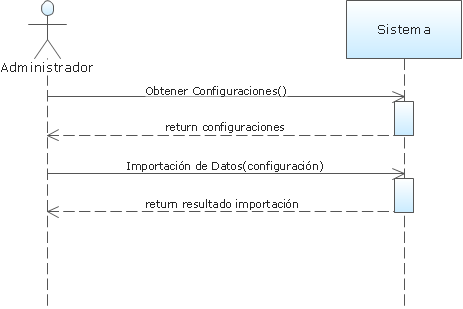
\includegraphics[width=0.7\textwidth]{DCImportacion.png}
  \caption{Modelo de Comportamiento Caso de Uso: Importación de datos}
  \label{image:compoimport}
\end{figure}
\subsubsection{Caso de Uso: Buscar en \gls{fulltext}}
\begin{figure}[H]
  \centering
     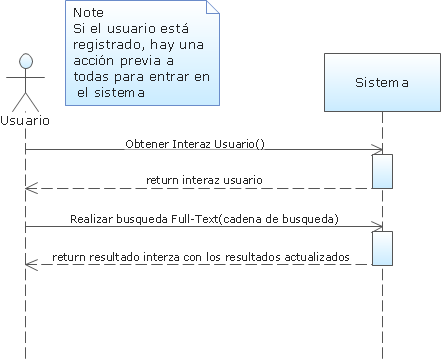
\includegraphics[width=0.7\textwidth]{DCfulltext.png}
  \caption{Modelo de Comportamiento aso de Uso: Buscar en \gls{fulltext}}
  \label{image:compofulltext}
\end{figure}
\subsubsection{Caso de Uso: Buscar \gls{metadato}}
\begin{figure}[H]
  \centering
     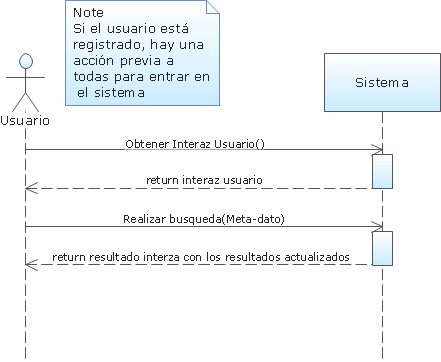
\includegraphics[width=0.7\textwidth]{DCmetadato.png}
  \caption{Modelo de Comportamiento Caso de Uso: Buscar \gls{metadato}}
  \label{image:compobusmeta}
\end{figure}
\subsubsection{Caso de Uso: Detalles de documento}
\begin{figure}[H]
  \centering
     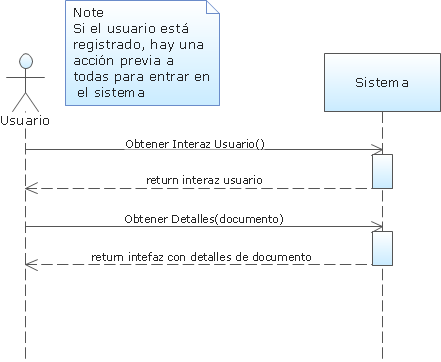
\includegraphics[width=0.7\textwidth]{DCDetalles.png}
  \caption{Modelo de Comportamiento Caso de Uso: Detalles de documento}
  \label{image:compodetalles}
\end{figure}
\subsubsection{Caso de Uso: Eliminar filtro}
\begin{figure}[H]
  \centering
     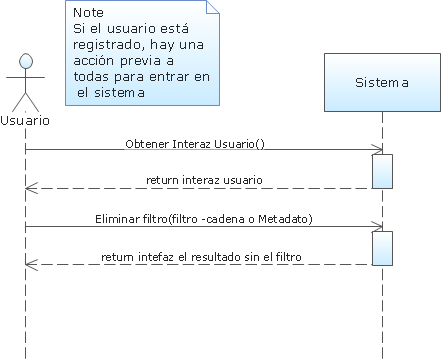
\includegraphics[width=0.7\textwidth]{DCeliminar.png}
  \caption{Modelo de Comportamiento Caso de Uso: Eliminar filtro}
  \label{image:compoelimina}
\end{figure}
\subsubsection{Caso de Uso: Cambiar lista de resultados}
\begin{figure}[H]
  \centering
     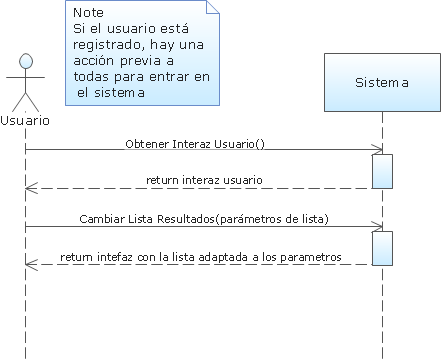
\includegraphics[width=0.7\textwidth]{DCcambialista.png}
  \caption{Modelo de Comportamiento Caso de Uso: Cambiar lista de resultados}
  \label{image:compocambia}
\end{figure}
\subsubsection{Caso de Uso: Resaltar \gls{metadato}}
\begin{figure}[H]
  \centering
     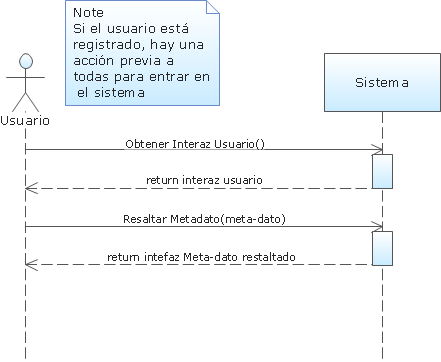
\includegraphics[width=0.7\textwidth]{DCresaltaMetadato.png}
  \caption{Modelo de Comportamiento Caso de Uso: Resaltar \gls{metadato}}
  \label{image:compresalmeta}
\end{figure}
\subsubsection{Caso de Uso: Resaltar \glspl{metadato} de documento}
\begin{figure}[H]
  \centering
     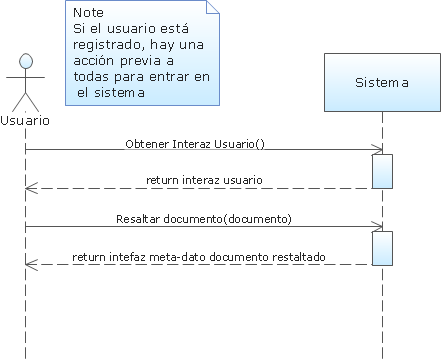
\includegraphics[width=0.7\textwidth]{DCresaltaDocu.png}
  \caption{Modelo de Comportamiento Caso de Uso: Resaltar \glspl{metadato} de documento}
  \label{image:comporesaldoc}
\end{figure}
\subsubsection{Caso de Uso: Mostrar grupo en grafo}
\begin{figure}[H]
  \centering
     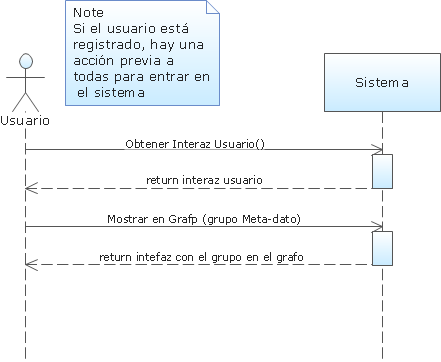
\includegraphics[width=0.7\textwidth]{DCmostrarGrupo.png}
  \caption{Modelo de Comportamiento Caso de Uso: Mostrar grupo en grafo}
  \label{image:compogropopgrafo}
\end{figure}


\section{\IfLanguageName{english}{User-interface Model}{Modelo de Interfaz de Usuario}} 
%En esta sección se deberá incluir un prototipo de baja fidelidad o mockup de la interfaz de usuario del sistema. Además, es preciso elaborar un diagrama de navegación, reflejando la secuencia de pantallas a las que tienen acceso los diferentes roles de usuario y la conexión entre éstas.

A continuación mostramos unos prototipos de baja fidelidad de la interfaz de usuario. En la imagen \ref{image:mockup1} podemos ver la estructura de la pantalla general de la aplicación.\\

\begin{figure}[h!]
  \centering
     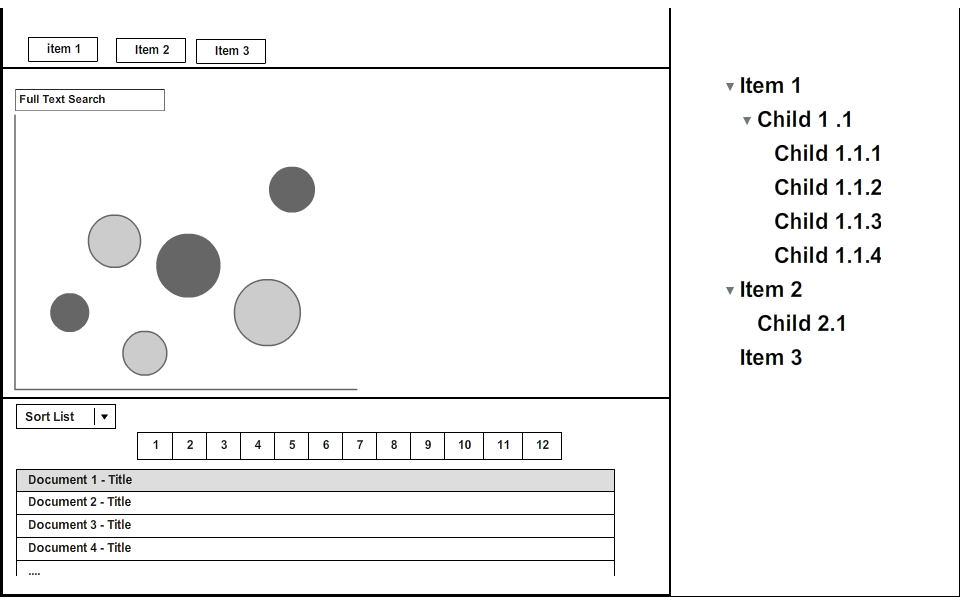
\includegraphics[width=0.8\textwidth]{mock1.png}
  \caption{Mockup - pantalla general \gls{kf2}}
  \label{image:mockup1}
\end{figure}

Cuando en usuario visualiza los detalles de un documento la pantalla tiene una semejanza a la expuesta en la imagen \ref{image:mockup2}.

\begin{figure}[h!]
  \centering
     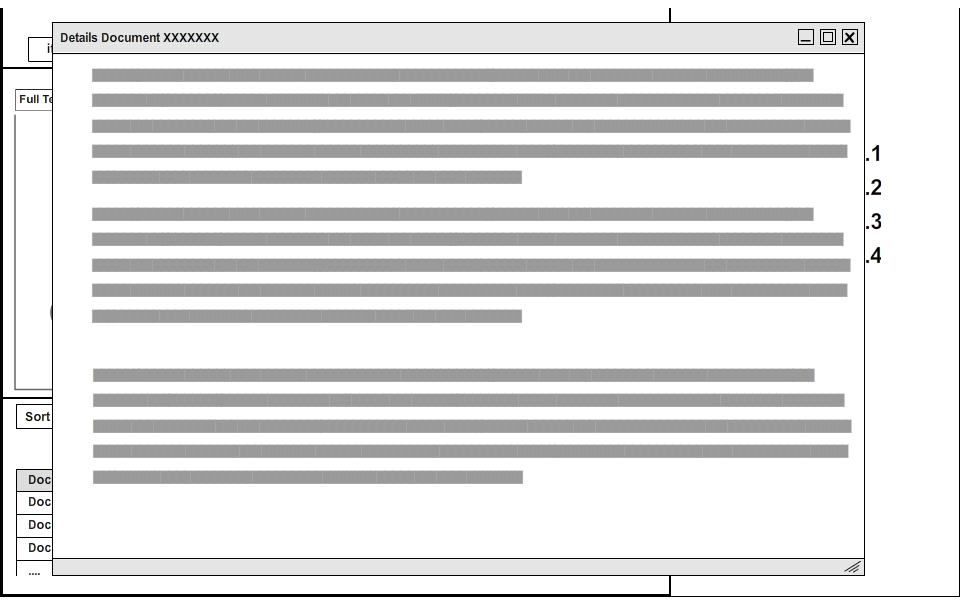
\includegraphics[width=0.8\textwidth]{mock2.png}
  \caption{Mockup - pantalla de detalles en \gls{kf2}}
  \label{image:mockup2}
\end{figure}


\chapter{\IfLanguageName{english}{System Design}{Diseño del Sistema}}
% ------------------------------------------------------------------------------
% Este fichero es parte de la plantilla LaTeX para la realización de Proyectos
% Final de Grado, protegido bajo los términos de la licencia GFDL.
% Para más información, la licencia completa viene incluida en el
% fichero fdl-1.3.tex

% Copyright (C) 2012 SPI-FM. Universidad de Cádiz
% ------------------------------------------------------------------------------

% En esta sección se recoge la arquitectura general del sistema de información, la parametrización del software base (opcional), el diseño físico de datos, el diseño detallado de componentes software y el diseño detallado de la interfaz de usuario.

\section{\IfLanguageName{english}{System Architecture}{Arquitectura del
Sistema}} 
%En esta sección se define la arquitectura general del sistema de información, especificando la infraestructura tecnológica necesaria para dar soporte al software y la estructura de los componentes que lo forman.

En este apartado de la documentación se expone la arquitectura general del proyecto \gls{kf2}, especificando la infraestructura tecnológica necesaria para dar soporte al software y la estructura de los componentes que lo forman.


\subsection{Ámbito y Contexto del Sistema}
En la figura \ref{image:level0} se representa la arquitectura de \gls{kf2} en su contexto. En ella se aprecia cómo esta aplicación interacciona con sus entidades externas.

\begin{figure}[H]
  \centering
     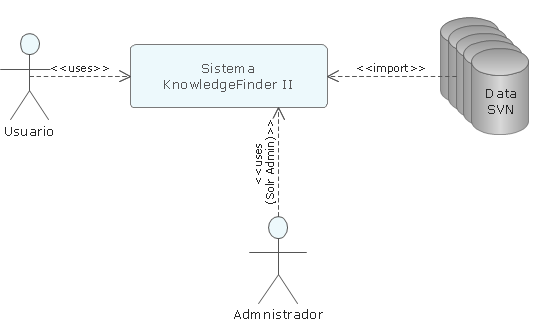
\includegraphics[width=0.8\textwidth]{Nivel0.png}
  \caption{Diagrama del ámbito y contexto de la arquitectura del sistema}
  \label{image:level0}
\end{figure}

\subsection{\IfLanguageName{english}{Hardware Architecture}{Arquitectura
Física}}

% En este apartado, describimos los principales elementos hardware que forman la arquitectura física de nuestro sistema, recogiendo por un lado los componentes del entorno de producción y los componentes de cliente.\\

% Se debe incluir un modelo de despliegue en el cual se describe cómo los elementos software son desplegados en los elementos hardware. También se incluyen las especificaciones y los requisitos del hardware (servidores, etc.), así como de los elementos software (sistemas operativos, servicios, aplicaciones, etc.) necesarios.
A continuación se va a describir el sistema de \gls{hardware} necesario que conforman la arquitectura física de nuestro sistema. En la figura \ref{image:deploview} podemos diferenciar los siguientes componentes:

\begin{itemize}

	\sitem{Cliente}
    Representa el \gls{hardware} que utiliza el usuario para acceder a los serivicios ofrecidos por \gls{kf2}. Éstos están dispolibles para ser usados por un navegador web o por un \gls{software} que permita el acceso a \glspl{sw}.
    
  	\sitem{Servidor para \gls{liferay} (\gls{tomcat})}
    Para alojar la instancia de \gls{liferay} que contendrá el \gls{sw} y el \gls{portlet} para la web de \gls{kf2} es necesario el \gls{hardware} apropiado para contener un servidor de \gls{tomcat}.
    
  \sitem{Servidor para \gls{solr}}
  El \gls{motorbusqueda} \gls{solr} puede estar instalado en varios tipos de servidores (\gls{tomcat}, \gls{jetty}, \dots). Para ello se requiere \gls{hardware} que pueda proporcionar alguno de estos. \Gls{solr} puede residir, por ejemplo, en la misma instancia de \gls{tomcat} donde se encuentra \gls{liferay} en ejecución.\\
  
  Este servidor debe tener acceso a los repositorios remotos o a una copia de trabajo local de \gls{svn} para el proceso de importación de los datos.
  
  \sitem{Control de acceso (nota)}
  Como medida de seguridad, se recomienda proteger el acceso a la instancia de \gls{solr} \cite{solrsecurity}. Para ello se pueden disponer de varias medidas de seguridad, por ejemplo un \gls{firewall}.
\end{itemize}

\begin{figure}[H]
  \centering
     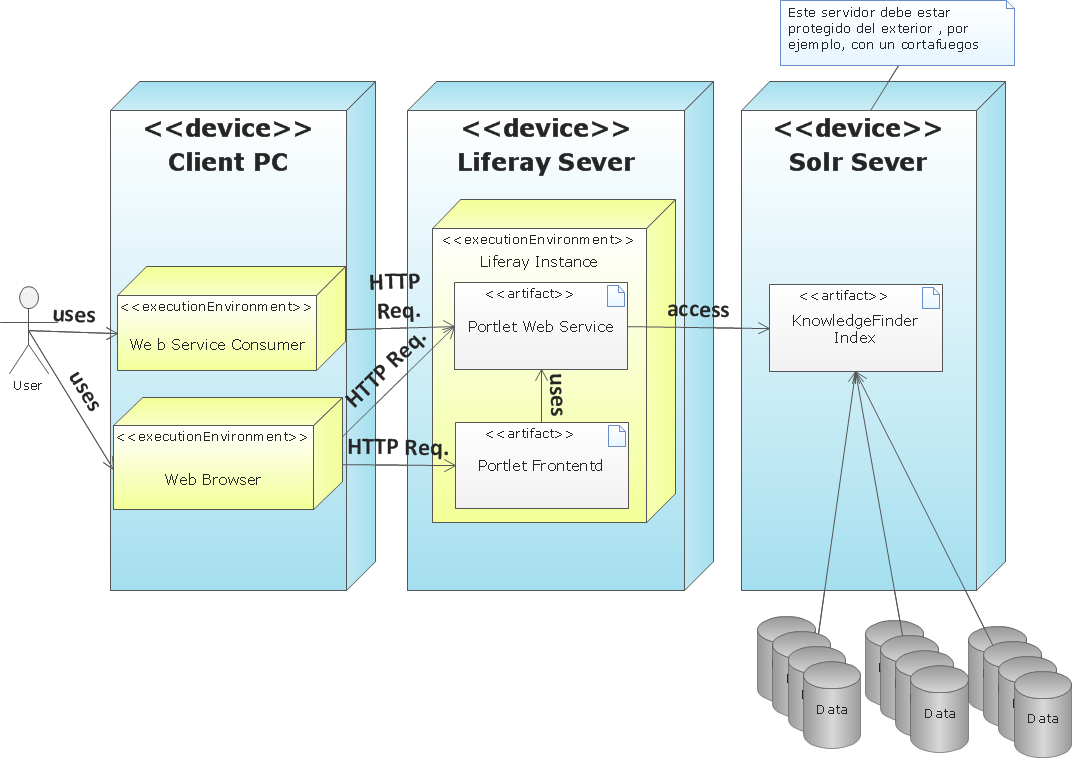
\includegraphics[width=\textwidth]{Despliegue.png}
  \caption{Diagrama de \gls{despliegue} para el proyecto \gls{kf2}}
  \label{image:deploview}
\end{figure}

\subsection{\IfLanguageName{english}{Software Architecture}{Arquitectura Lógica}} 

La arquitectura de diseño especifica la forma en que los artefactos software interactúan entre sí para lograr el comportamiento deseado en el sistema. En esta sección se muestra la comunicación entre el software base seleccionado, los componentes reutilizados y los componentes desarrollados para cumplir los requisitos de la aplicación. También se recogen los servicios de sistemas externos con los que interactúa nuestro sistema.\\

%Se debe incluir un diagrama de componentes que muestre en un alto nivel de abstracción los artefactos que conforman el sistema.\\

\subsection{Modelo Vista Controlador en \kfII}
Como se expuso en en apartado \ref{subsubsection:mvc}, el proyecto \gls{kf2} sigue una arquitectura de \gls{software} basada en el \gls{mvc}. A continuación se detalla cómo es el diseño aplicando esta arquitectura.



\begin{itemize}
	\sitem{El Modelo}
    En el caso de \gls{kf2} sería principalmente el índice de búsqueda. La información está almacenada en éste y es accesible gracias a la \gls{api} que proporciona el \gls{motorbusqueda}. 
    
    \sitem{El Controlador}
    El intermediario entre la vista y el índice de búsqueda es un 
\gls{sw} alojado en \gls{liferay}. De esta forma, el controlador tiene acceso a los roles del usuario definidos en \gls{liferay} que actualmente está usando la aplicación para definir su comportamiento. La respuesta del \gls{sw} variará para distintas combinaciones de roles de usuarios.
    
    \sitem{La Vista}
    Para el proyecto \gls{kf2} la vista representaría la página web donde se aloja la visualización y todos sus componentes. Es el interfaz principal del usuario para interactuar con el sistema.
\end{itemize}


\subsection{Desglose de Componentes}
\label{section:blocks}

Basándonos en el esquema expuesto en \cite{arc42} vamos a describir el la arquitectura del \gls{software} de \gls{kf2} por vistas de construcción. Comenzando por un nivel de abstracción donde se muestran los artefactos que conforman el sistema, se desglosará cada uno de ellos en sus componentes internas.\\

\subsubsection{Nivel 1 - Building View}
En la imagen \ref{image:level1} se puede ver como interactúa las distintos componentes del sistema \gls{kf2}. En ella también se aprecian las interfaces externas y los tres subsistemas principales que serán descritos en el siguiente nivel.
\begin{itemize}
	\sitem{Panel de administración de \gls{solr}} Interfaz para activar la importación de los datos.
    \sitem{Repositorios \gls{svn}} Conjunto de repositorios \gls{svn} desde donde se obtienen los datos.
    \sitem{Navegador de cliente} El usuario final interacciona directamente con el sistema usando un navegador web.
\end{itemize}

\begin{figure}[H]
  \centering
     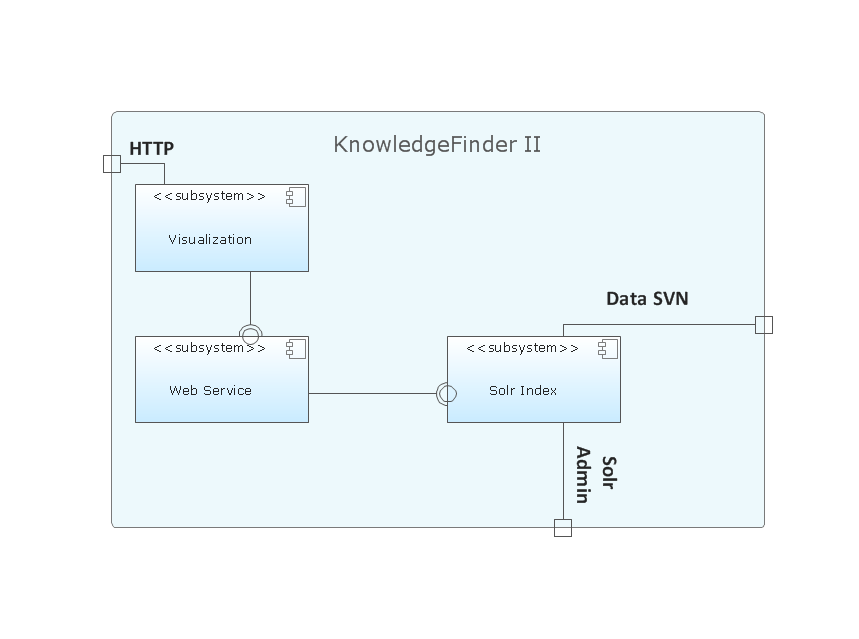
\includegraphics[width=\textwidth]{Nivel1.png}
  \caption{Nivel 1 - Building View \gls{kf2}}
  \label{image:level1}
\end{figure}


\subsubsection{Nivel 2 - Building View}
\label{subsubsection:n2building}
\sparagraph{Índice de búsqueda en \gls{solr}}
Este subsistema es responsable de la importación de la información para el índice de búsqueda de \gls{solr} desde los repositorios \gls{svn}. También se encarga de proporcionar estos datos importados a través de una \gls{api}. \\

Este subsistema de descompone los siguientes elementos representados en la imagen \ref{image:level2-solr}:
\begin{itemize}
	\sitem{\gls{svn} Crawler}
    Componente encargado de extraer los ficheros de \gls{svn} junto con todas sus propiedades. Recorre todo el repositorio (local o remoto) y empaqueta todas los elementos del repositorio.
    \sitem{\gls{svn} DataPicker}
    Componente encargado de transformar las extraer las propiedades de los elementos proporcionados por el crawler y empaquetarlos en objetos iterables de \gls{java}.
    \sitem{\gls{svn} Parser}
	Extrae las propiedades del \gls{svn} en formato \gls{json} y las prepara para la importación.
    \sitem{\gls{svn} DataImport}
    Se encarga de configurar y coordinar el proceso de importación.
    \sitem{\gls{solr} Tranformers}
    Transforma los datos durante la importación para adaptarlo a los requisitos específicos del índice.
    \sitem{\Gls{solr}}
    Instancia de \gls{solr} donde reside el índice importado. Proporciona la interfaz para importar y consultar los datos a través de una \gls{api} y un \gls{ui} web para su administración.
\end{itemize}

\begin{figure}[H]
  \centering
     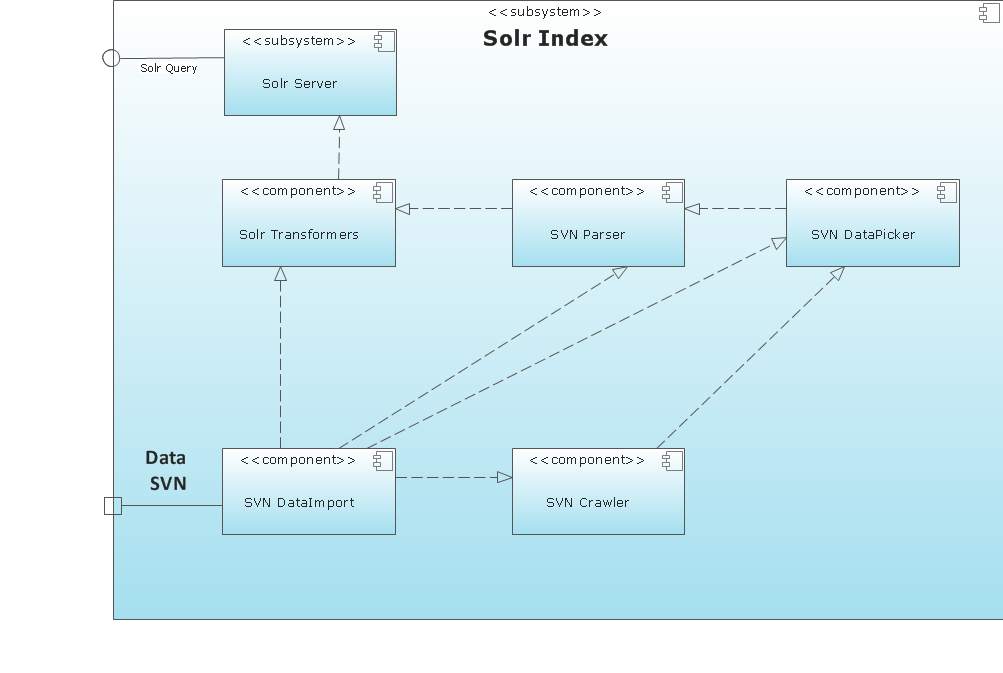
\includegraphics[width=\textwidth]{Nivel2Index.png}
  \caption{Nivel 2 - Building View Índice \gls{solr}}
  \label{image:level2-solr}
\end{figure}


\sparagraph{\Gls{sw}}
Este subsistema provee un \gls{sw} que permite acceder a los datos proporcionados por el índice de búsqueda \gls{solr}. Como muestra la imagen \ref{image:level2-sw}, se descompone en los siguientes elementos:
\begin{itemize}
	\sitem{KnowedgeFinder Service}
    Encargado de recibir las peticiones del \gls{sw} (get-document, get-nodes) y adaptar sus parámetros a la \gls{api} de \gls{solr}. Como resultado de las peticiones, crea una respuesta en formato \gls{json} con los valores pertinentes.
    \sitem{User-Query Factory}
    Elemento encargado de transformar las peticiones a la \gls{api} de \gls{solr} en función de los roles del usuario actual. 
\end{itemize}

\begin{figure}[H]
  \centering
     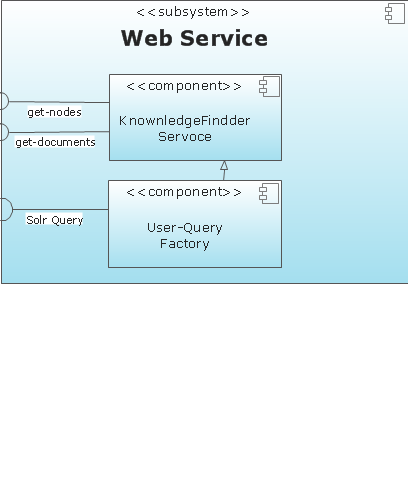
\includegraphics[width=0.5\textwidth]{Nivel2Webservice.png}
  \caption{Nivel 2 - Building View \Gls{sw}}
  \label{image:level2-sw}
\end{figure}

\sparagraph{Visualización}
El subsistema de visualización se encarga de proporcionar la \gls{ui} a través de elementos gráficos. A grandes rasgos, muestra la información obtenida a través del \gls{sw} de forma intuitiva y atractiva para el usuario. En la imagen \ref{image:level2-visual} se encuentran reflejados sus componentes y las relaciones entre ellos:

\begin{itemize}
	\sitem{TemplateController}
    Controlador que genera una página de \gls{jsp} para una \gls{url} definida por el administrador. 
    
    \sitem{Filters Loader}
    Este componente crea los filtros necesarios a partir de los \glspl{metadato} obtenido en peticiones al \gls{sw}.
    
    \sitem{Página \gls{html}}
    La página \gls{jsp} obtiene la información del TemplateController genera una página \gls{html}. Con los Filters Loader crea variables que son necesarias por todos los componentes \gls{js}.
    \sitem{Main.js}
    Encargado de cargar todos los componentes de \gls{js}. También coordina los evento del usuario y el comportamiento de los componentes entre ellos.
  	\sitem{d3.knowledgefinder.graph.js}  
    Componente encargado de crear un grafo que representa los \glspl{metadato} y las relaciones entre ellos.
    \sitem{d3.knowledgefinder.modal.js}
    Componente que genera una ventana emergente con los detalles de un documento previamente seleccionado de la lista de resultados.
    \sitem{d3.knowledgefinder.result.js}
	Lista los documentos obtenidos durante la consulta y los organiza usando un sistema de \gls{paginacion}.
    \sitem{d3.knowledgefinder.selection.js}
    Componente encargado de mostrar una lista de botones con los actuales parámetros de búsqueda. A través de esta lista el usuario puede consultar y desactivar los elementos que componen la búsqueda.
    \sitem{d3.knowledgefinder.table.js}
    La tabla generada por el componente de Página \gls{html} es manipulada a través de este componente de acuerdo a los resultados y búsquedas.
    \sitem{d3.knowledgefinder.urlquery.js}
    Componente auxiliar para manipular los parámetros y facilitar al resto de componentes de la visualización la comunicación con el \gls{sw}. 
\end{itemize}
\begin{figure}[H]
  \centering
     \includegraphics[width=\textwidth]{Nivel2Visualization.png}
  \caption{Nivel 2 - Building View Visualización}
  \label{image:level2-visual}
\end{figure}

%Existen diferentes patrones o estilos arquitectónicos. En los sistemas web de información es común la utilización del patrón Layers (Capas), con el cual estructuramos el sistema en un número apropiado de capas, de forma que todos los componentes de una misma capa trabajan en el mismo nivel de abstracción y los servicios proporcionados por la capa superior utilizan internamente los servicios proporcionados por la capa inmediatamente inferior. Habitualmente se tienen las siguientes capas:

\begin{comment}
\paragraph*{\IfLanguageName{english}{Presentation Tier (frontend)}{Capa de
presentación (frontend)}} Este grupo de artefactos software conforman la capa de presentación del sistema, incluyendo tanto los componentes de la vista como los elementos de control de la misma.

\paragraph*{\IfLanguageName{english}{Application Tier}{Capa de negocio}}
Este grupo de artefactos software conforman la capa de negocio del sistema, incluyendo los elementos del modelo de dominio y los servicios (operaciones del sistema).

\paragraph*{\IfLanguageName{english}{Data Tier}{Capa de persistencia}}
Este grupo de artefactos software conforman la capa de integración del sistema, incluyendo las clases de abstracción para el acceso a datos (BD o sistema de ficheros) o a sistemas heredados.\\

Es común que a la capa de negocio y de datos de los sistemas web, se denomine conjuntamente como backend o modelo de la aplicación.

Opcionalmente, podemos disponer de un conjunto de artefactos software que pueden ser usados por elementos de cualquiera de las capas del sistema y que fundamentalmente proporcionan servicios relacionados con requisitos no funcionales (calidad).
\end{comment}

\begin{comment}
\section{\IfLanguageName{english}{Parameterization of the Based
Software}{Parametrización del software base}} 
\question{Tengo que poner algo en mi caso aquí????}
\todo[inline]{En esta sección, se detallan las
modificaciones a realizar sobre el software base, que son requeridas para la correcta construcción del sistema. En esta sección incluiremos las  actuaciones necesarias sobre la interfaz de administración del sistema, sobre el código fuente o sobre el modelo de datos.}
\end{comment}

\section{\IfLanguageName{english}{Physical Data Design}{Diseño Físico de Datos}}
\begin{comment}
En esta sección se define la estructura física de datos que utilizará el sistema, a partir del modelo de conceptual de clases, de manera que teniendo presente los requisitos establecidos para el sistema de información y las particularidades del entorno tecnológico, se consiga un acceso eficiente de los datos.
La estructura física se compone de tablas, índices, procedimientos almacenados, secuencias y otros elementos dependientes del SGBD a utilizar.
\end{comment}
La estructura física de los datos que utiliza el sistema es el índice de búsqueda de \gls{solr}. Su definición se describe en el esquema. Estos esquemas deben definirse dependiendo de las necesidades de cada instancia del \gls{framework} \gls{kf2}.\\

A continuación se detalla en la tabla \ref{table:index} en detalle la estructura del índice de búsqueda una vez que la importación ha finalizado (instancia del proyecto \gls{strada} de \gls{kf2}). En ella se puede observar, entre otros datos, qué campos se utilizan para la búsqueda \gls{fulltext}, los campos que son creados en el momento de la importación (dinámicos), qué campos son usados para la búsqueda en el índice, etcétera .

\begin{center}
\begin {table}[H]
    \begin{tabular}{| l | c | l | c | c | c | p{5cm} |}
    \hline
    \rot{\textbf{Campo}} & \rot{\textbf{Obligatorio}} & \rot{\textbf{Tipo}} & \rot{\textbf{Múltiple}} & \rot{\textbf{Index}} & \rot{\textbf{Stored}} & \rot{\textbf{Notas}}		\\ \hline
    id  			& X & string 		&   & X & X	& Unique Key  	 	\\ \hline
    title 			& X & text			&   & X & X & \Gls{fulltext}    \\ \hline
    description     &   & text    	 	&	&  	& X	& \Gls{fulltext}    \\ \hline
    keywords 		&   & string 		& X & X & X	& \Gls{fulltext}    \\ \hline
    categories      &  	& string 		& X &  	& X	& 					\\ \hline
    filePath 		& 	& string 		& 	&   & X	&				\\ \hline
    institute 		&   & string 		& 	&   & X & Generado durante la importación \\ \hline
 timePeriodOfDataCollection &  & string &   &   & X	&				\\ \hline
 startTimePeriodOfDataCollection &  & date &   & X & X	&				\\ \hline
 endTimePeriodOfDataCollection &  & date &   & X & X	&				\\ \hline
 startDateDate		 &  & date 			&   & X & X	&				\\ \hline
 temporalCoverage    &  & string 		&   &  	& X	& 					\\ \hline
 startTemporalCoverage &  & date &   & X & X	&				\\ \hline
 endTemporalCoverage &  & date &   & X & X	&				\\ \hline
 spatialCoverage &  & string & X &   & X	&				\\ \hline
 world &  & string & X & X  & 	& Generado desde spatialCoverage \\ \hline
 regionsWorld &  & string & X & X  & 	& Generado desde spatialCoverage \\ \hline
 countries &  & string & X & X  & 	& Generado desde spatialCoverage \\ \hline
 regions &  & string & X & X  & 	& Generado desde spatialCoverage \\ \hline
 size\_author & & int & & & X & Generado desde authors \\ \hline
 contentcreationdatetime & & int & & X &  & Propiedad interna de \gls{svn} \\ \hline
 contentmodificationdatetime & & int & & X &  & Propiedad interna de \gls{svn} \\ \hline
 author\_uid\_* & & string & & & X & Generado desde authors (campo dinámico), \Gls{fulltext} \\ \hline
 author\_firstName\_* & & string & & & X & Generado desde authors (campo dinámico), \Gls{fulltext} \\ \hline
 author\_lastName\_* & & string & & & X & Generado desde authors (campo dinámico), \Gls{fulltext} \\ \hline
 author\_mail\_* & & string & & & X & Generado desde authors (campo dinámico), \Gls{fulltext} \\ \hline
 author\_organization\_* & & string & & & X & Generado desde authors (campo dinámico), \Gls{fulltext} \\ \hline
  category\_* & & string & X & X & X & Generado desde categories (campo dinámico), \Gls{fulltext} \\ \hline
    \end{tabular}
    \caption{Tabla resumen del esquema de \gls{kf2} de \gls{solr} para el proyecto \gls{strada}}
    \label{table:index}
  \end{table}
\end{center}

\begin{comment}

% Reemplazado por la vista de procesos 
\section{\IfLanguageName{english}{Detailed Component Design}{Diseño detallado de Componentes}}
Para cada uno de los módulos funcionales del sistema debemos realizar un diagrama de secuencia, para definir la interacción existente entre las clases de objetos que permitan responder a eventos externos.
\end{comment}

\section{Vista de Procesos}
Siguiendo nuevamente el esquema expuesto  en \cite{arc42}, en esta sección se describe el comportamiento de los componentes del sistema descritos en la sección \ref{section:blocks} como elementos de ejecución.\\

A continuación se describen los escenarios más interesantes y los casos de uso más importantes del sistema destacando qué componentes de los subsistemas y qué subsistemas tienen mayor relevancia con mayor transcendencia para el lector de esta documentación.

\subsection{Iniciación de la Visualización}
La página web que contiene la visualización debe ser inicializada en el servidor cuando un usuario realiza una consulta sobre la \gls{url} correcta.\\

El primer paso lo realiza el controlador del \gls{portlet}. Éste adquiere los filtros y establece los elementos del menú a través de llamadas al \gls{sw}. Una vez que obtiene todos los datos, genera la página \gls{jsp}. Cuando la página ha sido creada se inicializan todos los componentes de \gls{js} usando nuevamente llamadas al \gls{sw}. Este proceso se describe con más detalles en la imagen \ref{image:runtime-init}.


\begin{figure}[H]
  \centering
  	\includegraphics[width=\textwidth]{SE2init.png}
  \caption{Diagrama de Secuencia - Iniciación de la Visualización}
  \label{image:runtime-init}
\end{figure}

\subsection{Ejecución de Consulta}
Cuando el usuario ejecuta una consulta añadiendo o eliminando algún filtro, por ejemplo, seleccionando un elemento del menú o introduciendo un valor en el campo \gls{fulltext} el sistema debe obtener el nuevo estado para todos los componentes de la \gls{ui}.\\

Concretamente, la lista de resultados debe mostrar el nuevo conjunto de documentos fruto de la nueva consulta. El grafo debe calcular los nuevos valores para sus componentes y redibujarlos en función de éstos. El menú debe adecuarse igualmente al nuevo estado de la aplicación. Para todo ello, se realizan diversas consultas al \gls{sw} de forma asíncrona adaptadas a cada componente. El gráfico representado en la imagen \ref{image:runtime-query} esquematiza este comportamiento.

\begin{figure}[H]
  \centering
  	\includegraphics[width=1\textwidth]{SEChangeQ.png}
  \caption{Diagrama de Secuencia - Ejecución de Consulta}
  \label{image:runtime-query}
\end{figure}

\subsection{Modificación del Grafo de Exploración}
Sin modificar la consulta, el usuario puede modificar los grupos que se muestran en el grafo a través de las opciones del menú. El grafo obtiene los valores para este nuevo estado a través de consultas al \gls{sw}. Con el diagrama de secuencia de la imagen \ref{image:runtime-graph} se representa este proceso.

\begin{figure}[H]
  \centering
  	\includegraphics[width=1\textwidth]{SEChangeGraph.png}
  \caption{Diagrama de Secuencia - Modificación del Grafo de Exploración}
  \label{image:runtime-graph}
\end{figure}

\subsection{Modificación de la Lista de Resultados}
La lista de resultados está organizada en páginas y ordenada por según la elección del usuario dentro de unas posibles opciones. Tanto si el usuario cambia de página usando los elementos de la \gls{paginacion} o selecciona otro criterio de ordenación el sistema debe actualizar los elementos de esta lista a través de consultas al \gls{sw}. En la imagen \ref{image:runtime-results} se expone el diagrama de secuencia para estas acciones.

\begin{figure}[H]
  \centering
  	\includegraphics[width=1\textwidth]{SEChangeResults.png}
  \caption{Diagrama de Secuencia - Modificación de la Lista de Resultados}
  \label{image:runtime-results}
\end{figure}


\begin{comment}
Alternative terms:

Dynamic view
Process view
Workflow view
This view describes the behavior and interaction of the system’s building blocks as runtime elements (processes, tasks, activities, threads, …).

Select interesting runtime scenarios such as:

How are the most important use cases executed by the architectural building blocks?
Which instances of architectural building blocks are created at runtime and how are they started, controlled, and stopped.
How do the system’s components co-operate with external and pre-existing components?
How is the system started (covering e.g. required start scripts, dependencies on external systems, databases, communications systems, etc.)?
 

Note: The main criterion for the choice of possible scenarios (sequences, workflows) is their architectural relevancy. It is not important to describe a large number of scenarios. You should rather document a representative selection.

Candidates are:

1.The top 3 – 5 use cases

2.System startup

3.The system’s behavior on its most important external interfaces

4.The system’s behavior in the most important error situations

 

Motivation
Esp. for object-oriented architectures it is not sufficient to specify the building blocks with their interfaces, but also how instances of building blocks interact during runtime.

This view explains how the blocks interact, how they provide their functionality, how the systems works.

 

Form
Document the chosen scenarios using UML sequence diagrams, activity diagrams or communications diagrams. Enumerated lists are sometimes feasible.

Using object diagrams you can depict snapshots of existing runtime objects as well as instantiated relationships. The UML allows to distinguish between active and passive objects.
\end{comment}

\section{\IfLanguageName{english}{Detailed Design of the User Interface}{Diseño detallado de la Interfaz de Usuario}}
\begin{comment}
En esta sección se detallarán las interfaces entre el sistema y el usuario, incluyendo un prototipo de alta fidelidad con el diseño de la IU. Se definirá el comportamiento de las diferentes pantallas, indicando qué ocurre en los distintos componentes visuales de la interfaz cuando aparecen y qué acciones se disparan cuando el usuario trabaja con ellas.
\end{comment}
En esta sección se va a describir con detalle el diseño y el comportamiento de la \gls{ui} del \gls{framework} \gls{kf2}. Para esta versión se definen dos pantallas; la pantalla principal y la pantalla de detalles de documento.


\subsection{Pantalla Principal}
La pantalla principal de la aplicación se puede observar en la imagen \ref{image:uiprincipal}. Como la figura indica, se diferencian cinco componentes que a continuación se exponen.

\begin{figure}[h!]
  \centering
  	\includegraphics[width=1\textwidth]{general_ap.png}
  \caption{Pantalla principal}
  \label{image:uiprincipal}
\end{figure}

\subsubsection{Grapo de Exploración}
Representa el elemento más importante de la visualización. En el grafo se representa los filtros aplicables a los documentos que concuerdan con la búsqueda aplicada. Cada filtro representa un nodo y las aristas las relación entre nodos, el número de documentos con ambos filtros. El tamaño de los nodos y el grosor de las aristas está directamente relacionado con el número de documentos para cada elemento.\\

Cuando el usuario pulsa sobre algún nodo o alguna arista del grafo se aplican los correspondientes filtros.

\subsubsection{Menú}
Ofrece todos los posibles filtros de \glspl{metadato} disponibles. Están ordenados por números de documentos afectados por el filtro y se reordenan cuando estos valores cambian.\\

Se agrupan en, como máximo, dos subniveles siendo el elemento principal de cada grupo. Estos grupos se representan en modo acordeón con un posible \gls{scroll} sobre las listas de filtros.\\

A través de un botón en los encabezados de los grupos, el usuario podrá seleccionar qué grupos serán mostrados en el gráfico y pulsando sobre los elementos del menú, qué filtros se han de aplicar para búsqueda.
 
\subsubsection{Lista de Resultados}
Los resultado de la búsqueda realizada en cada momento es mostrada en una lista con los títulos de los documentos. Esta lista está dividida usando un sistema de \gls{paginacion}.\\

Cuando el usuario pulsa sobre algún elemento de la lista, se despliega una sección en forma de acordeón con la descripción del documento seleccionado y un botón para desplegar sus detalles en una ventana emergente (ver sección \ref{subsection:detalles}). También se puede desplegar/plegar este acordeón para todos los elementos de la lista pulsando un botón y  puede ser ordenada por varios criterios seleccionables a través de un menú \textit{Drop-down}.

\subsubsection{Filtros Aplicados}
En la parte superior de la pantalla principal se muestran los filtros actuales y cadenas de búsquedas aplicadas. Pulsando sobre ellos se eliminan de los criterios de búsqueda.

\subsubsection{Comportamientos Transversales}
Los componentes anteriormente descritos se relacionan entre sí a través de los siguientes cuando el usuario se posiciona en un elemento del grafo o sobre uno del menú:
    \begin{itemize}
    	\item El grafo muestra resaltado respecto al resto de elementos el subgrafo compuesto por las componentes conexas del filtro en cuestión.
   		\item En el menú de elementos se resalta el filtro.
   		\item En la lista de resultados se resaltan los que tienen relación ese filtro.
   \end{itemize}

\subsubsection{Campo \gls{fulltext}}
Entre el grafo de exploración y los filtros aplicados  se encuentra un simple formulario para la introducción de cadenas de búsqueda. En ella, el usuario puede de definir su propias cadenas de búsqueda.

\subsection{Pantalla de Detalles de Documento}
\label{subsection:detalles}
Como se ha explicado antes, los detalles de los documentos se exponen en una ventana emergente. En la imagen \ref{image:uidetalles} se observa la simpleza de ésta. Se muestran los campos configurados para cada usuario y la opción de cerrar la ventana para volver a la pantalla anterior.

\begin{figure}[h!]
  \centering
  	\includegraphics[width=1\textwidth]{hightpopp.png}
  \caption{Pantalla detalles de documento}
  \label{image:uidetalles}
\end{figure}




\chapter{\IfLanguageName{english}{Implementation}{Construcción del Sistema}}
% ------------------------------------------------------------------------------
% Este fichero es parte de la plantilla LaTeX para la realización de Proyectos
% Final de Grado, protegido bajo los términos de la licencia GFDL.
% Para más información, la licencia completa viene incluida en el
% fichero fdl-1.3.tex

% Copyright (C) 2012 SPI-FM. Universidad de Cádiz
% ------------------------------------------------------------------------------


\begin{comment}
Este capítulo trata sobre todos los aspectos relacionados con la implementación del sistema en código, haciendo uso de un determinado entorno tecnológico. 
\end{comment}

En este capitulo se detallarán los elementos relacionados con la implementación del \gls{framework} \gls{kf2} y el entorno tecnológico donde se ha desarrollado.


\section{\IfLanguageName{english}{Development environment}{Entorno de
Construcción}}
\begin{comment}
En esta sección se debe indicar el marco tecnológico utilizado para la construcción del sistema: entorno de desarrollo (IDE), lenguaje de programación, herramientas de ayuda a la construcción y despliegue, control de versiones, repositorio de componentes, integración contínua, etc.
\end{comment}
A continuación vamos a describir las herramientas utilizadas  durante el desarrollo resumidas en la sección \ref{section:dlr}.\\

En entorno de desarrollo empleado fue \gls{eclipse} Kepler SR2 utilizándose \gls{java} 1.7 con \gls{jsdk} y \gls{js} como lenguajes de programación principales para el desarrollo del producto.\\

Para controlar las versiones del producto se utilizó un repositorio \gls{svn} instalado en el \gls{dlr} para los proyectos internos el \gls{scvss}. Este repositorio se utilizó conjuntamente con el gestor de proyectos \gls{mantis} y \gls{jenkins} para la integración continua. Ambas herramientas empleadas por el \gls{scvss} para todos sus proyectos.\\

En el \gls{scvss} se dispone de un propio repositorio de \gls{maven} para la gestión y construcción de proyectos. Por ello, esta herramienta fue esencial para la construcción y distribución del proyecto desarrollado.\\

Como se comentó anteriormente, \gls{kf2} utiliza \gls{liferay} como portal y \gls{solr} para el índice de búsqueda. Por este motivo se utilizó una instancia de este portal (versión 6.2.1 CE GA2) funcionando sobre un servidor \gls{tomcat} 7 y de \gls{solr} 4.8.1 sobre \gls{jetty} en su configuración de ejemplo.\\

Para hacer más cómodo el desarrollo, se empleó el \gls{software} \gls{jrebel} 5.6.1 que ayuda a la aplicación automática de la aplicación de las modificaciones en el código \glslink{despliegue}{desplegado}. También se utilizó el \gls{framework} \gls{wiremock} 1.18 para simular los servicios durante la fase \textit{Extended Static Prototype}(ver apartado \ref{subsubsection:aplicandoextre}).\\

En la tabla \ref{table:pluginseclipse} se listan los \glspl{plugin} usados conjuntamente con \gls{eclipse} para integrar las herramientas anteriormente descritas en el entorno de desarrollo y completar la funcionalidad de este \gls{ide}.

\begin{center}
\begin {table}[H]
\centering
    \begin{tabular}{ | l   c   p{7cm} |}
    \hline
    \textbf{\Gls{plugin}} &  \textbf{Versión} & \textbf{Comentario} \\ \hline
    %%%%%%
     Subclipse & 1.10.5 & \Gls{plugin} para \gls{svn} \\ \hline
     Mylyn Mantis Connector & 3.11.0 & \Gls{plugin} para \gls{mantis} \\ \hline
     Hudson/Jenkins Mylyn Builds Connector & 1.4.0 & \Gls{plugin} para \gls{jenkins} \\ \hline
     \Gls{jrebel} for \gls{eclipse} & 5.6.2 & \Gls{plugin} para \gls{jrebel} \\ \hline 
     \Gls{liferay} \gls{ide} & 2.1.1 GA2 & \Gls{plugin} para \gls{liferay} \\ \hline 
     m2e-liferay & 2.1.1 GA2 & \Gls{plugin} para uso conjunto de \gls{maven} y \gls{liferay} \\ \hline
     
    \end{tabular}
    \caption{\Glspl{plugin} usados en \gls{eclipse} durante el desarrollo.}
    \label{table:pluginseclipse}
    \end{table}
\end{center}

\section{\IfLanguageName{english}{Source Code}{Código Fuente}}
\begin{comment}
Organización del código fuente, describiendo la utilidad de los diferentes ficheros y su distribución en paquetes o directorios. Asimismo, se incluirá algún extracto significativo de código fuente que sea de interés para ilustrar algún algoritmo o funcionalidad específica del sistema.
\end{comment}

Como se ha descrito en apartados anteriores, la aplicación está descompuesta en tres subsistemas. A continuación se va a describir el código de cada uno de ellos y los ficheros  claves para la configuración para el proyecto usado como ejemplo \gls{strada}.

\subsection{Índice Solr}
La importación de la información contenida en los repositorios \gls{svn} esta implementada principalmente en los siguientes paquetes de \gls{java}:
\begin{itemize}
	\item \textbf{de.dlr.xps.server.handler.dataimport.crawler}
    En este paquete se implementa la funcionalidad del subsistema \gls{svn} Crawler
    (ver \ref{subsubsection:n2building})
    \item \textbf{de.dlr.xps.server.handler.dataimport.datapicker}
    En este paquete se implementa la funcionalidad del subsistema \gls{svn} DataPicker
    (ver \ref{subsubsection:n2building})
    \item \textbf{de.dlr.xps.server.handler.dataimport.parser}
    En este paquete se implementa la funcionalidad del subsistema \gls{svn} Parser
    (ver \ref{subsubsection:n2building})
    \item \textbf{de.dlr.xps.server.handler.dataimport.transformer}
    En este paquete se implementa la funcionalidad del subsistema \gls{solr} Transformers
    (ver \ref{subsubsection:n2building})
    \item \textbf{de.dlr.xps.server.handler.dataimport}
    En este paquete se implementa la funcionalidad del subsistema \gls{svn} DataImport
    (ver \ref{subsubsection:n2building})
\end{itemize}

Los archivos de configuración para el proyecto \gls{strada} indican cómo debe de realizarse la importación y el esquema del índice de búsqueda. En el fragmento de código \ref{code:import} es observa el fichero \textit{data-conf.xml} resumido para un origen de datos.

\begin{listing}[H]
\begin{minted}[linenos,
               numbersep=5pt,
               frame=single,
               fontsize=\scriptsize,
               framesep=2mm]{xml}
                
<dataConfig>
 <dataSource name="StradaSVN" type="SVNDataSource" />
 <document>
  <entity name="strada" 
   processor="SVNEntityProcessor"
   transformer="
      RegexTransformer,
      TemplateTransformer,
      de.dlr.xps.server.handler.dataimport.transformer.GenerateIdTransformer,
      de.dlr.xps.server.handler.dataimport.transformer.LStripTransformer,
      de.dlr.xps.server.handler.dataimport.transformer.ExcludeValuesTransformer,
      de.dlr.xps.server.handler.dataimport.transformer.CategoriesIdTransformer,
      de.dlr.xps.server.handler.dataimport.transformer.CategoriesSeparatedTransformer,
      de.dlr.xps.server.handler.dataimport.transformer.DateIncompleteFormatTransformer,
      de.dlr.xps.server.handler.dataimport.transformer.SpatialCoverageTransformer,
      de.dlr.xps.server.handler.dataimport.transformer.DictionaryListTransformer"
   
   query="/home/efrain/Escritorio/dlr_software/svn/local/CS">
   <!-- RegexTransformer -->
   <field column="timePeriodOfDataCollection"
          regex="(.*)\s-\s(.*)" 
          groupNames="startCollection,endCollection"/>
   <!-- RegexTransformer -->
   <field column="temporalCoverage" 
   		  regex="(.*)\s-\s(.*)" 
          groupNames="startCoverage,endCoverage"/>
   <!-- DateIncompleteFormatTransformer -->
   <field column="startTemporalCoverage" 
          sourceColName="startCoverage" 
          parseToDate="start" 
          regex="^(?&lt;year&gt;\d{4})(\D)?(?&lt;month&gt;\d{2})?(\D)?(?&lt;day&gt;\d{2})$"/>
   <field column="endTemporalCoverage" 
          sourceColName="endCoverage" 
          parseToDate="end" 
          regex="^(?&lt;year&gt;\d{4})(\D)?(?&lt;month&gt;\d{2})?(\D)?(?&lt;day&gt;\d{2})?$"/>
   <!-- ExcludeValuesTransformer, CategoriesIdTransformer, CategoriesSeparatedTransformer -->
   <field column="contentCategories" 
         name="categories" 
         exclude="import/cs-exclude-categories.txt" 
         categories="import/cs-categories.json" 
         categories_id_name="categories_id" 
         categories_split_prefix="category_"/>
   
   <!-- LStripTransformer, ExcludeValuesTransformer, SpatialCoverageTransformer -->
   <field column="spatialCoverage" 
          lstrip="import/strip-spatial.txt" 
          exclude="import/exclude-spatial.txt"
          spatialColumns="world,regionsWorld,countries,regions"
          worldFile="import/world.txt" 
          worldRegionsFile="import/worldRegions.txt"/>
   <!-- DictionaryListTransformer -->
   <field column="authors" 
          dictionaryId="author" />
  </entity>
  ...
 </document>
</dataConfig>
	\end{minted}
	\caption{Ejemplo de importación de datos en \gls{kf2} para \gls{strada}}
	\label{code:import}
\end{listing}

Para definir el esquema del índice \gls{solr} se utiliza el fichero \textit{schema.xml}. En el código \ref{code:schema} se oberva como se ha definido éste para \gls{strada}.

\begin{listing}[H]
\begin{minted}[linenos,
               numbersep=5pt,
               frame=single,
               fontsize=\scriptsize,
               framesep=2mm]{xml}
                
<?xml version="1.0" encoding="UTF-8" ?>
<schema name="knowledgefinder" version="1.5">
 <fields>
  <field name="_version_" type="long" indexed="true" stored="true" />
  <field name="id" type="string" indexed="true" stored="true" required="true" multiValued="false" />
  <field name="title" type="text_general" indexed="true" stored="true" multiValued="false" required="true" />
  <field name="description" type="text_general" indexed="false" stored="true" multiValued="false"/>
  <field name="keywords" type="string" indexed="true" stored="true" multiValued="true" />
  <field name="categories" type="string" indexed="false" stored="true" multiValued="true" />
  <field name="filePath" type="string" indexed="false" stored="true" multiValued="false" />
  <field name="institute" type="string" indexed="true" stored="true" multiValued="false" />
  <field name="timePeriodOfDataCollection" type="string" indexed="false" stored="true" multiValued="false" />
  <field name="startTimePeriodOfDataCollection" type="tdate" indexed="true" stored="true" multiValued="false" />
  <field name="endTimePeriodOfDataCollection" type="tdate" indexed="true" stored="true" multiValued="false" />
  <field name="startDateDate" type="tdate" indexed="true" stored="true" multiValued="false" />
  <field name="temporalCoverage" type="string" indexed="false" stored="true" multiValued="false" />
  <field name="startTemporalCoverage" type="tdate" indexed="true" stored="true" multiValued="false" />
  <field name="endTemporalCoverage" type="tdate" indexed="true" stored="true" multiValued="false" />
  <field name="spatialCoverage" type="string" indexed="false" stored="true" multiValued="true" />
  <field name="world" type="string" indexed="true" stored="false" multiValued="true" />
  <field name="regionsWorld" type="string" indexed="true" stored="false" multiValued="true" /> 
  <field name="countries" type="string" indexed="true" stored="false" multiValued="true" />
  <field name="regions" type="string" indexed="true" stored="false" multiValued="true" />
  <field name="size_author" type="int" indexed="false" stored="true" multiValued="false" />
  <field name="____contentcreationdatetime____" type="int" indexed="true" stored="false" multiValued="false" />
  <field name="____contentmodificationdatetime____" type="int" indexed="true" stored="false" multiValued="false" />
  <dynamicField name="author_uid_*" type="string" indexed="false" stored="true" multiValued="false" />
  <dynamicField name="author_firstName_*" type="string" indexed="false" stored="true" multiValued="false" />
  <dynamicField name="author_lastName_*" type="string" indexed="false" stored="true" multiValued="false" />
  <dynamicField name="author_mail_*" type="string" indexed="false" stored="true" multiValued="false" />
  <dynamicField name="author_organization_*" type="string" indexed="false" stored="true" multiValued="false" />
  <field name="full_text_search" type="text_general" indexed="true" stored="false" multiValued="true" />
  <field name="title_sort" type="alphaOnlySort" indexed="true" stored="true" multiValued="false" />

  <copyField source="title" dest="full_text_search" />  
  <copyField source="title" dest="title_sort" />
  <copyField source="description" dest="full_text_search" />
  <copyField source="keywords" dest="full_text_search" />
  <copyField source="categories" dest="full_text_search" />
  <copyField source="world" dest="full_text_search" />
  <copyField source="regionsWorld" dest="full_text_search" />
  <copyField source="countries" dest="full_text_search" />
  <copyField source="regions" dest="full_text_search" />
  <copyField source="author_uid_*" dest="full_text_search" />
  <copyField source="author_firstName_*" dest="full_text_search" />
  <copyField source="author_lastName_*" dest="full_text_search" />
  <copyField source="author_mail_*" dest="full_text_search" />
  <copyField source="author_organization_*" dest="full_text_search" />
  <!-- From Transformer Categories -->
  <dynamicField name="category_*" type="string" indexed="true" stored="true" multiValued="true" />
  <copyField source="category_*" dest="full_text_search" />
  <!-- Not logger required -->
  <field name="categories_id" type="ignored" indexed="false" stored="false" multiValued="true" />
  <dynamicField name="*" type="ignored" indexed="true" stored="true" multiValued="true" />
 </fields>
 <uniqueKey>id</uniqueKey>
 ...
	\end{minted}
	\caption{Ejemplo de esquema del índice \gls{solr} en \gls{kf2} para \gls{strada}}
	\label{code:schema}
\end{listing}

\subsection{Servicio Web}
El \gls{sw} que corre sobre \gls{liferay} está organizado en tres paquetes de \gls{java}:
\begin{itemize}
	\sitem{de.dlr.xps.server.knowledgefinder.webservice.solr}
    En este paquete se encuentra el código para obtener la configuración del \gls{sw}.
    \sitem{de.dlr.xps.server.knowledgefinder.webservice.solr.query}
    Para personalizar y configurar las consultas para cada tipo de rol se han definido en este paquete unas clases en modo de ejemplo para los supuestos roles de usuario.
    \sitem{de.dlr.xps.server.knowledgefinder.webservice.service}
    En este paquete se encuentran las clases que definen la \gls{api} del \gls{sw} y su implementación.
\end{itemize}

Para configurar el \gls{sw} y definir el punto de conexión con el servidor \gls{solr} se tiene el fichero \textit{webservice.properties}. En el código \ref{code:service} se puede observar un ejemplo de configuración para el proyecto \gls{strada}.

\begin{listing}[H]
\begin{minted}[linenos,
               numbersep=5pt,
               frame=single,
               framesep=2mm]{bash}
##
## Solr connection
##
	solr.scheme=http
	solr.host=localhost
	solr.port=8983
	solr.username=username
	solr.password =password
	solr.core=solr/strada

    \end{minted}
	\caption{Ejemplo de configuración del \gls{sw} en \gls{kf2} para \gls{strada}}
	\label{code:service}
\end{listing}

\subsection{Visualización}
El subsistema de visualización se puede dividir en grupos de código con propositos claramente diferenciados:

\begin{itemize}
	\sitem{de.dlr.xps.server.knowledgefinder.frontend.controller}
    En este paquete se encuentra el código encargado de inicializar el \gls{portlet} con la para la página web.
    \sitem{de.dlr.xps.server.knowledgefinder.frontend.menu}
    A través de un fichero de configuración, genera el el menú para incorporarlo a la visualización.
    \sitem{Directorio styles-sass}
    En este directorio se encuentra el código en \gls{sass} para definir los estilos de la aplicación.
    \sitem{Directorio js}
    Todo el código \gls{js} creado para la visualización se encuentra alojado en este directorio junto con las librerías empleadas.
\end{itemize}

\subsubsection{Menú}

Para configurar el menú se utiliza el fichero en formato \gls{json} \textit{menuConfiguration.json}. La tabla \ref{table:formatomenu} muestra el formato de los elementos de configuración que lo componen. En el código \ref{code:categorias} se muestra la configuración para \gls{strada}.

\begin{center}
\begin {table}[H]
	\centering
    \begin{tabular}{ | l l |}
    \hline
    \textbf{Propiedad} & \textbf{Comentario} \\ \hline
    %%%%%%
    id & Valor identificativo del elemento  \\ \hline
    name & Nombre mostrado en el menú  \\ \hline
    query & Búsqueda aplicada para el elemento principal \\ \hline
    cssClass & Clase de CSS para el grupo \\ \hline
    subItemsFacet & Consulta facet para obtener los subelementos \\ \hline
    collapsed & Indica si se debe mostrar el grupo plegado \\ \hline
    scrollable & Indica se utiliza un \gls{scroll} para el grupo \\ \hline
    subItems & Lista de subelementos de configuración \\ \hline
    children\_filter & Indica si los subelementos deben ignorarse \\ \hline
    \end{tabular}
    \caption{Formato de los elementos de configuración para el menú}
    \label{table:formatomenu}
  \end{table}
\end{center}


\begin{listing}[H]
\begin{minted}[linenos,
               numbersep=5pt,
               frame=single,
               fontsize=\scriptsize,
               framesep=2mm]{json}
{
  "menuItems": [
    {
      "id": "CAT",
      "name": "Categories",
      "cssClass": "CAT-filter",
      "collapsed": false,
      "scrollable": false,
      "subItems": [
        {
          "id": "PT",
          "name": "Passenger Transport",
          "subItemsFacet": "category_Passenger Transport",
          "cssClass": "CAT-PT-filter",
          "collapsed": true,
          "scrollable": true,
          "children_filter": true
        },
...
      ]
    },
    {
      "id": "SC",
      "name": "Spatial Coverage",
      "cssClass": "SC-filter",
      "collapsed": false,
      "scrollable": false,
      "subItems": [
        {
          "id": "SCW",
          "name": "World",
          "subItemsFacet": "world",
          "cssClass": "SC-SCW-filter",
          "collapsed": true,
          "scrollable": true,
          "children_filter": false
        },
        {
          "id": "SCWR",
          "name": "Word regional level",
          "subItemsFacet": "regionsWorld",
          "cssClass": "SC-SCWR-filter",
          "collapsed": true,
          "scrollable": true,
          "children_filter": true
        },
...
      ]
    },
    {
      "id": "KW",
      "name": "Keywords",
      "cssClass": "red",
      "query": "keywords:[\"\" TO *]",
      "cssClass": "KW-filter",
      "subItemsFacet": "keywords",
      "collapsed": true,
      "scrollable": true,
      "subItems": []
    }
  ]
}
    \end{minted}
	\caption{Ejemplo de configuración del menú en \gls{kf2} para \gls{strada}}
	\label{code:categorias}
\end{listing}

\subsubsection{\gls{js}} 
En la tabla \ref{table:javascriptplug} se muestra las herramientas externas usadas para este proyecto de \gls{js}.

\begin{center}
\begin {table}[H]
	\centering
    \begin{tabular}{ | l l |}
    \hline
    \textbf{Herramienta} & \textbf{Comentario} \\ \hline
    %%%%%%
    \gls{d3} & Herramienta principal de la visualización  \\ \hline
    \gls{bootstrap} & Código para componentes visuales \\ \hline
    jQuery & Herramienta requerida por otras \\ \hline
    Queue.js & Ejecución en paralelo de código \gls{js} \\ \hline
    URI.js & Herramienta para el manejo de \glspl{url} \\ \hline
    History.js & Manipulación del historial para \gls{html5} \\ \hline
    mCustomScrollbar.js & \Gls{scroll} en menú \\ \hline
    \end{tabular}
    \caption{Herramientas de \gls{js} usadas}
    \label{table:javascriptplug}
  \end{table}
\end{center}


\subsubsection{Estilos \gls{css}}

Todos los estilos de la aplicación se han personalizado basándose en la librería \gls{bootstrap} y se han escrito usando \gls{sass}. Para la compilación y aplicación de todos los ficheros fuentes de \gls{sass} se ha usado el \gls{software} \gls{compass}.\\

Para configurar los colores de los elementos gráficos de visualización de la \gls{ui} se ha definido en un único fichero de  \gls{sass}, \textit{\_filter\_colors.scss}, la paleta de colores a usar. En los códigos \ref{code:colorssass} y \ref{code:colorssass2} se muestran cómo es para \gls{strada}.

\begin{listing}[H]
\begin{minted}[linenos,
               numbersep=5pt,
               frame=single,
               fontsize=\scriptsize,
               framesep=2mm]{sass}
               
/* Germany colors
$CAT-color: lighten(#000000, 50%);
$SC-color: #CD0000;
$KW-color: #FFCC00
*/

/* DLR colors */
$CAT-color: rgb(75, 128, 136);
$SC-color: rgb(73, 107, 169);
$KW-color: rgb(126, 75, 86);

$filterColors: (
   CAT-filter: $CAT-color,
   CAT-PT-filter: $CAT-color,
   CAT-T-filter: $CAT-color, 
   CAT-CT-filter: $CAT-color,
   CAT-EI-filter: $CAT-color,
   CAT-VT-filter: $CAT-color,
   CAT-IN-filter: $CAT-color,
   CAT-FDG-filter: $CAT-color,
   CAT-TMP-filter: $CAT-color, 
   
   SC-filter: $SC-color,
   SC-SCW-filter: $SC-color,
   SC-SCWR-filter: $SC-color, 
   SC-SCC-filter: $SC-color,
   SC-SCR-filter: $SC-color,
   
   KW-filter: $KW-color,
);

    \end{minted}
	\caption{Ejemplo de paleta de colores en \gls{kf2} para \gls{strada}}
	\label{code:colorssass}
\end{listing}

\begin{listing}[H]
\begin{minted}[linenos,
               numbersep=5pt,
               frame=single,
               fontsize=\scriptsize,
               framesep=2mm]{sass}
               
@each $filter, $color in $filterColors {
 .#{$filter} {
  /* Graph circles */
  &.gnode {
   > circle {
    fill: $color;
   }
  }
  /* Current selection */
  &.sel-filter {
   color: $color;
   border-color: $color;
  }
  /* Navigation table, selected */
  &.selected{
   .header-filter {
    background-color: rgba($color, 0.25);
   }
  }
 }
}
.CAT-filter {
 .header-group {
  color: white;
  background-color: map-get($filterColors, CAT-filter);
 }
 .header-filter {
  background-color: rgba(map-get($filterColors, CAT-filter), .1);
  
  > a {
   color: map-get($filterColors, CAT-filter);
  }
 }
 .header-subfilter { 
  .name {
   color: map-get($filterColors, CAT-filter);
  }
 }
}
/* Example, how to change color of a subfilter */
/*
.CAT-CT-filter {
 .header-filter {
  background-color: rgba(map-get($filterColors, CAT-CT-filter), .1);
  > a {
   color: map-get($filterColors, CAT-CT-filter);
  }
 }
 .header-subfilter { 
  .name {
   color: map-get($filterColors, CAT-CT-filter);
  }
 }
}
*/
...
    \end{minted}
	\caption{Ejemplo de aplicación de la paleta de colores en \gls{kf2} para \gls{strada}}
	\label{code:colorssass2}
\end{listing}


% \section{\IfLanguageName{english}{}{Scripts de Base de datos}}
% Organización del código fuente, describiendo la utilidad de los diferentes
% ficheros y su distribución en paquetes o directorios. Asimismo, se incluirá el
% script de algún disparador o un procedimiento almacenado, que sea de interés para ilustrar algún aspecto concreto de la gestión de la base de datos.

\chapter{\IfLanguageName{english}{Testing}{Pruebas del Sistema}}
% ------------------------------------------------------------------------------
% Este fichero es parte de la plantilla LaTeX para la realización de Proyectos
% Final de Grado, protegido bajo los términos de la licencia GFDL.
% Para más información, la licencia completa viene incluida en el
% fichero fdl-1.3.tex

% Copyright (C) 2012 SPI-FM. Universidad de Cádiz
% ------------------------------------------------------------------------------

% En este capítulo se presenta el plan de pruebas del sistema de información, incluyendo los diferentes tipos de pruebas que se han llevado a cabo, ya sean manuales (mediante listas de comprobación) o automatizadas mediante algún software específico de pruebas.

En este capítulo se explican el plan de pruebas del proyecto \gls{kf2}.

\section{\IfLanguageName{english}{Test Strategy}{Estrategia}}
% 1. En esta sección se debe incluir el alcance de las pruebas, hasta donde se pretende llegar con ellas, si se registrarán todas o sólo aquellas de un cierto tipo y cómo se interpretarán y evaluarán los resultados.

% 2. También, se incluirá el procedimiento a seguir para las pruebas de regresión, esto es, la repetición de ciertas pruebas para comprobar que nuevos cambios que se vayan introduciendo no originen errores en el software ya probado.

Por las características del producto, las pruebas de cada componente se han planteado de forma distinta:

\begin{itemize}
    \item{\textbf{Índice de búsqueda \gls{solr}}}
    Se han realizado pruebas a bajo nivel para comprobar el correcto funcionamiento de la lectura, transformación e importación de los datos en el servidor \gls{solr}.
    \item{\textbf{\Gls{sw}}}
    Este componente ha sido probado durante el proceso de desarrollo de la visualización. Por este motivo, junto con el carácter piloto del \gls{software} y la complejidad de los elementos implicados, no se ha desarrollado explícitamente ningún tipo de pruebas sobre el código.
    \item{\textbf{Visualización}}
    Este componente reúne la mayoría de los requisitos funcionales del usuario final. Por ello, se han realizado en él con una alta perseverancia durante todo el proceso de desarrollo las pruebas de sistemas.
\end{itemize}

\section{\IfLanguageName{english}{Testing Environment}{Entorno de Pruebas}}
% Incluir en este apartado los requisitos de los entornos hardware/software donde se ejecutarán las pruebas.

El conjunto de pruebas se ha realizado a tres niveles:
\begin{itemize}
    \item \textbf{Equipo de desarrollo} Las pruebas se han ejecutado en el equipo del programador durante el desarrollo.
    \item \textbf{Servidor de pruebas} Para ver el producto en funcionamiento en un equipo semejo a donde se pondrá en producción se ha dispuesto de un servidor de pruebas remoto.
    \item \textbf{\gls{jenkins}} Esta herramienta ha realizado y registrado el resultado de la fase de \gls{testing} durante el \gls{despliegue} de las distintas versiones intermedias del producto.
\end{itemize}

\section{\IfLanguageName{english}{Roles}{Roles}}
En desarrollador se encarga de realizar las pruebas durante todo el desarrollo del producto. 
% Describir en esa sección cuáles serán los perfiles y participantes necesarios para la ejecución de cada uno de los niveles de prueba.

Todas las pruebas unitarias y de integración han sido ejecutadas únicamente por el desarrollador y las herramientas automáticas.\\

El desarrollador tambíen ha comprobado cumplimiento de los requisitos realizando las pruebas de sistema durante el transcurso la creación del producto.\\

Conjuntamente con el personal de \gls{scvss} y de los institutos \gls{vf} y \gls{fw} asignados al proyecto, el desarrollador se ha encargado de las pruebas de aceptación.
% usando el servidor de pruebas anteriormente nombrado.

\section{\IfLanguageName{english}{Testing Levels}{Niveles de Pruebas}}
%En este sección se documentan los diferentes tipos de pruebas que se han llevado a cabo, ya sean manuales o automatizadas mediante algún software específico de pruebas.

\subsection{\IfLanguageName{english}{Unit Testing}{Pruebas Unitarias}}
El proceso de lectura de la información contenida en \gls{svn} y las transformaciones previas a la importación ha sido probado a través de pruebas unitarias para cada componente funcional.
% solr
% Las pruebas unitarias tienen por objetivo localizar errores en cada nuevo artefacto software desarrollado, antes que se produzca la integración con el resto de artefactos del sistema.

\subsection{\IfLanguageName{english}{Integration Testing}{Pruebas de
Integración}} 
% solr solrimport + solr in server
% Este tipo de pruebas tienen por objetivo localizar errores en módulos o subsistemas completos, analizando la interacción entre varios artefactos software.
Gracias al paquete para pruebas implementado en \gls{solr}, los elementos encargados de la importación han sido probados en un servidor \gls{solr} destinado a tal fin. De esta forma se aseguró que el código encargado de la importación funciona correctamente sobre la versión de \gls{solr} deseada.

\subsection{\IfLanguageName{english}{System Testing}{Pruebas de Sistema}}
% visualización y webservice
% En esta actividad se realizan las pruebas de sistema de modo que se asegure que el sistema cumple con todos los requisitos establecidos: funcionales, de almacenamiento, reglas de negocio y no funcionales. Se suelen desarrollar en un entorno específico para pruebas.
En lo que refiere al índice de búsqueda, se ha comprobado que el índice resultado de la importación contiene la información esperada. Para ello se ha comparado la información contenida en el repositorio \gls{svn} en formato \gls{json} con los datos del índice.\\

Por otra parte, para comprobar el correcto funcionamiento de la aplicación y que el sistema cumple con todos los requisitos establecidos se han realizado pruebas manuales a lo largo de la fase de implementación de la visualización y del \gls{sw}.\\

Con una lista que representa cada caso de uso establecido, se ha comprobado en cada versión de los componentes de visualización y \gls{sw} que los requisitos funcionales concluidos y los requisitos no funcionales han seguido estando satisfechos.

%\subsubsection{\IfLanguageName{english}{Functional Testing}{Pruebas Funcionales}} 
% Con estas pruebas se analiza el buen funcionamiento de la implementación de los flujos normales y alternativos de los distintos casos de uso del sistema.


% \subsubsection{\IfLanguageName{english}{Not-functional testing}{Pruebas No Funcionales}}
% Estas pruebas pretenden comprobar el funcionamiento del sistema, con respecto a los requisitos no funcionales identificados: eficiencia, seguridad, etc.


\subsection{\IfLanguageName{english}{Acceptance Testing}{Pruebas de Aceptación}}
% El objetivo de estas pruebas es demostrar que el producto está listo para el paso a producción. Suelen ser las mismas pruebas que se realizaron anteriormente pero en el entorno de producción. En estas pruebas, es importante la participación del cliente final.
Usando el servidor de pruebas anteriormente nombrado, se han realizado las pruebas de aceptación durante la fase cercana a la finalización del esta versión del \gls{framework} \gls{kf2}. Principalmente han consistido en la comprobación de las pruebas de sistema en el servidor.





% EPILOGO
\part{\IfLanguageName{english}{Epilogue}{Epílogo}}
\null\vfill

 
\vfill

\chapter{\IfLanguageName{english}{Reference Guide}{Manual de implantación y
explotación}}
% ------------------------------------------------------------------------------
% Este fichero es parte de la plantilla LaTeX para la realización de Proyectos
% Final de Grado, protegido bajo los términos de la licencia GFDL.
% Para más información, la licencia completa viene incluida en el
% fichero fdl-1.3.tex

% Copyright (C) 2012 SPI-FM. Universidad de Cádiz
% ------------------------------------------------------------------------------

Las instrucciones de uso del \gls{framework} \gls{kf2} aplicado al \gls{strada} se detallan a continuación.

\section{\IfLanguageName{english}{Introduction}{Introducción}}
% Resumen de los principales objetivos, ámbito y alcance del software desarrollado.

En el presente capitulo se desarrollará el manual de instalación y explotación del índice de búsqueda en \gls{solr}, del servicio web \glslink{despliegue}{desplegado} en \gls{liferay} y de la \gls{ui} en un \gls{portlet} del proyecto \gls{strada} implementado con el \gls{framework} \gls{kf2}.\\

Esta aplicación web permite consultar las bases de datos de ``\transmov'' de los institutos del \glsfirst{dlr} \glsfirst{fw} y \glsfirst{vf} conjuntamente los documentos de ambos portales ofreciendo un sistema de búsqueda avanzada y optimizada sobre los \glspl{metadato} de los documentos de los institutos involucrados.\\

El portal ofrece una visualización del conocimiento interactiva de los \glspl{metadato}  que representa las relaciones espaciales, temporales y contextuales entre los documentos y fuentes de datos. Esta representación aporta nuevos conocimientos que facilitan las tareas de investigación.\\




Este manual se divide en tres módulos que se tratarán de expondrán de forma independiente:
\begin{itemize}
	\item Índice \gls{solr}
	\item \Gls{sw} en \gls{liferay}
	\item \Gls{portlet} de visualización
\end{itemize}

\section{Requisitos generales previos}
A continuación se exponen los requisitos necesarios comunes a todos los módulos que se describirán en este manual.

\subsection{Java}
Basándonos en la documentación de \gls{solr} 4.8.1 \cite{solrinstall}, el servidor requiere la versión de \gls{jsdk} 7 o superior. Aunque impuesto por \gls{solr}, se recomienda usar la misma versión de \gls{jsdk} para los restantes módulos.\\

Una vez se tenga instalado, hay que configurar la variable del sistema $JAVA\_HOME$ para usar el \gls{jsdk} que acabamos de instalar.

\subsection{Eclipse}
\label{subsubsection:eclipsesolr}
Para el desarrollo de este software se recomienda utilizar el \gls{ide} \gls{eclipse}. Éste se puede descargar en la dirección oficial \url{http://www.eclipse.org/downloads/}.

\subsection{\maven{} 3}
La instalación de \gls{maven} se puede realizar en algunos sistemas operativos, como Ubuntu, desde los repositorios oficiales. Desde la dirección oficial (\url{http://maven.apache.org/download.html}) también se pueden descargar e instalar fácilmente.\\

Si no se ha configurado automáticamente durante el paso anterior, hay que crear una variable de sistema $M2\_HOME$ que apunte al directorio donde se ha instalado, por ejemplo:
\mbox{C:\textbackslash{}Program Files(x86)\textbackslash{}apache-maven-3.1.0}.\\

Si la organización cuenta con un repositorio de \gls{maven} propio, éste se puede añadir editando el fichero \textit{settings.xml} de \gls{maven}. Por ejemplo, para el \gls{scvss}, el repositorio apunta a \url{http://repo.sistec.dlr.de/nexus/content/groups/public/}.\\

Para usarlo conjuntamente con \gls{eclipse} (apartado \ref{subsubsection:eclipsesolr}) se recomienda instalar el \gls{plugin} Maven2Eclipse desde la dirección \url{http://download.eclipse.org/technology/m2e/releases}

\subsection{Cliente \Gls{svn}}
Para poder obtener el código y trabajar con el repositorio \gls{svn} es necesario instalar un cliente de \gls{svn} 1.7 o superior.\\

También se puede optar por instalar directamente un \gls{plugin} para \gls{eclipse} que incluya este cliente, por ejemplo Subclipse que está disponible bajo la dirección \url{http://subclipse.tigris.org/update_1.10.x}.

\subsection{\Gls{mantis} y \gls{jenkins}}
\Gls{eclipse} se conecta con \gls{mantis} y \gls{jenkins} a través de Mylyn. Este \gls{plugin} está disponible en la dirección \url{http://download.eclipse.org/mylyn/releases/latest}.\\

Para configurar en Mylyn \gls{mantis} en \gls{eclipse} siga los siguientes pasos:
\begin{enumerate} 
	\item Window > Show View > Task List
	\item Click on Add MyLyn Support
	\item Install connector (Mantis)
	\item Boton derecho en task view, add query
	\item Add new repository
		\subitem Type: Mantis
		\subitem Path: https://www.sistec.dlr.de/mantis
		\subitem User/Pass: Tus credenciales
		\subitem Validate
	\item Crear las consultas (queries) deseadas.
\end{enumerate}

A continuación, la configuración de Mylyn con \gls{jenkins}:
\begin{enumerate}
	\item Window > Show View > Builds
	\item Add build
		\subitem Type: Hudson [Jenkins]
		\subitem Path: https://ci.sc.dlr.de/jenkins
		\subitem User/Pass: Tus credentials
		\subitem Validate
	\item Elegir los builds de \gls{kf2} de la lista.
\end{enumerate}

\section{Índice Solr}
\label{section:manualsolr}
En este apartado se describe el manual de desarrollo, instalación y explotación del sistema de importación de datos y su aplicación en un servidor \gls{solr}.

\subsection{\IfLanguageName{english}{Requirements}{Requisitos previos}}

\subsubsection{Apache \gls{solr} 4.8.1}
\label{subsubsection:solrinstall}
Desde la dirección \url{http://www.apache.org/dyn/closer.cgi/lucene/solr/4.8.1} nos podemos descargar \gls{solr}. Una vez descargado y descomprimido en un directorio, por ejemplo ``UnzipDirectory'', ejecutamos el servidor \gls{jetty} de ejemplo (código \ref{code:jettysorl}).\\

\begin{listing}[H]
    \begin{minted}[linenos,
               numbersep=5pt,
               frame=single,
               framesep=2mm]{bash}

java -jar [UnzipDirectory]/solr-4.8.1/example/start.jar
    \end{minted}
    \caption{Ejemplo de ejecución inicial de \gls{solr} en \gls{jetty}}
    \label{code:jettysorl}
\end{listing}


Si todo ha funcionado correctamente, \gls{solr} estaría accesible en la dirección \url{http://localhost:8983/solr}.


%\section{\IfLanguageName{english}{}{Inventario de componentes}}
%Lista de los componentes hardware y software que se incluyen en la versión del
% producto.

\subsection{\IfLanguageName{english}{Installation and Setup
procedures}{Procedimientos de instalación}}
%Procedimientos de instalación y configuración de cada componente hardware y software (base y desarrollado) para asegurar la correcta instalación y explotación del sistema, así como aquellos procedimientos necesarios de migración/carga de datos.

\subsubsection{Obtención del \gls{software}}
Checkout desde \gls{svn} el índice desde \url{https://svn.sistec.dlr.de/svn/xps/xps-server/branches/visual/solrIndex/} si no se dispone de una copia de trabajo.\\

Checkout desde \gls{svn} del sistema de importación desde \url{https://svn.sistec.dlr.de/svn/xps/xps-server/branches/visual/de.dlr.xps.server.knowledgefinder.handler.dataimport/} si no se dispone de una copia de trabajo.\\

\subsubsection{Construcción del \gls{software}}
Situándonos en el directorio donde se ha realizado el checkout, ejecutamos las lineas expuestas en el código \ref{code:solrbuild1} y \ref{code:solrbuild2}.

\begin{listing}[H]
    \begin{minted}[linenos,
               numbersep=5pt,
               frame=single,
               framesep=2mm]{bash}

cd ./de.dlr.xps.server.knowledgefinder.handler.dataimport/
mvn clean install
    \end{minted}
    \caption{Construcción con \gls{maven} de DataImport}
    \label{code:solrbuild1}
\end{listing}

\begin{listing}[H]
    \begin{minted}[linenos,
               numbersep=5pt,
               frame=single,
               framesep=2mm]{bash}

cd ../solrIndex/
mvn clean install
    \end{minted}
    \caption{Construcción con \gls{maven} de índice de búsqueda}
    \label{code:solrbuild2}
\end{listing}


A través de \gls{eclipse} se puede realizar también siguiendo estos pasos:
\begin{itemize}
	\item Añadir un nuevo ``Maven Run Configuration'' usando como directorio base\\
          $\$\{workspace\_loc:\/de.dlr.xps.server.knowledgefinder.handler.dataimport\}$\\
          y como ``goal'' clean install para construir el sistema de importación.
	\item Añadir un nuevo ``Maven Run Configuration'' usando como directorio base\\ 			  $\$\{workspace\_loc:\/solr\_index\}$\\
		  y como ``goal'' clean install para construir el índice.
\end{itemize}

\subsubsection{\Gls{despliegue} en el \gls{solr}}
Para concluir se debe de configurar \gls{solr} para que utilice el índice. Para ello se debe ejecutar el servidor \gls{jetty} como se vio en el apartado \ref{subsubsection:solrinstall} pero indicando la variable $solr.solr.home$ (código \ref{code:solrdeploy}).

\begin{listing}[H]
    \begin{minted}[linenos,
               numbersep=5pt,
               frame=single,
               framesep=2mm]{bash}

java -jar -Dsolr.solr.home={workspace_loc}/solr_index
[UnzipDirectory]/solr-4.8.1/example/start.jar
    \end{minted}
    \caption{Ejemplo de ejecución de \gls{solr} en \gls{jetty} con el índice de \gls{strada}}
    \label{code:solrdeploy}
\end{listing}

\subsubsection{Configuración del índice}
Después de la instalación, hay que configurar el origen de los datos.\\

Los datos se pueden obtener desde el repositorio \gls{svn} (\url{https://svn-dmz.sistec.dlr.de/svn/xps/fw-test-data/}) y configurar el índice con la ruta de la copia de trabajo local (código \ref{code:importlocal}).

\begin{listing}[H]
    \begin{minted}[linenos,
               numbersep=5pt,
               frame=single,
               framesep=2mm]{xml}

...
<entity name="strada"
processor="SVNEntityProcessor"
transformer="..."
query="/KFdata/dat/CS"
...
>
...
<entity name="fw"
processor="SVNEntityProcessor"
transformer="..."
query="/KFdata/dat/FW"
...
>
...
    \end{minted}
    \caption{Configuración del índice desde copia de trabajo local de \gls{svn}}
    \label{code:importlocal}
\end{listing}


Otra opción es que la importación se realice directamente leyendo el repositorio de \gls{svn} remoto. Para ello hay que configurar también las credenciales para acceder al mismo (código \ref{code:importremote})\\

\begin{listing}[H]
    \begin{minted}[linenos,
               numbersep=5pt,
               frame=single,
               framesep=2mm]{xml}

...
<entity name="strada"
processor="SVNEntityProcessor"
transformer="..."
query="https://svn-dmz.sistec.dlr.de/svn/xps/fw-test-data/dat/CS"
username="usernameSVN"
password="passwordSVN"
...
>
...
<entity name="fw"
processor="SVNEntityProcessor"
transformer="..."
query="https://svn-dmz.sistec.dlr.de/svn/xps/fw-test-data/dat/FW"
username="usernameSVN"
password="passwordSVN"
...
>
...
    \end{minted}
    \caption{Configuración del índice desde repositorio remoto de \gls{svn}}
    \label{code:importremote}
\end{listing}


\subsubsection*{Configuración en servidor}
En el código \ref{code:solrdebian} se muestra un ejemplo de configuración para servicio en una máquina de la familia Debian.
\begin{listing}[H]
    \begin{minted}[linenos,
               numbersep=5pt,
               frame=single,
               framesep=2mm]{bash}

#!/bin/bash
#startup script for the Solr server
#
# description: Starts and stops the Solr with Jetty daemon.
# processname: solr (java)
# pidfile: /var/run/solr.pid
JAVA_7_HOME=/usr/lib/jvm/jdk1.7.0_60/
SOLR_HOME=/home/lima_ef/solrIndex/
JETTY_HOME=/opt/solr-4.8.1/example/
STOP_PORT=8079
STOP_KEY=keyStopSolr
case $1
in
start)
export JAVA.HOME=$JAVA_7_HOME
java -jar -Dsolr.solr.home=$SOLR_HOME -DSTOP.PORT=$STOP_PORT 
          -Djetty.home=$JETTY_HOME
/opt/solr-4.8.1/example/start.jar --start
;;
stop)
export JAVA.HOME=$JAVA_7_HOME
java -jar -Dsolr.solr.home=$SOLR_HOME -DSTOP.PORT=$STOP_PORT 
          -Djetty.home=$JETTY_HOME
/opt/solr-4.8.1/example/start.jar --stop
;;
restart)
export JAVA.HOME=$JAVA_7_HOME
java -jar -Dsolr.solr.home=$SOLR_HOME -DSTOP.PORT=$STOP_PORT 
          -Djetty.home=$JETTY_HOME
/opt/solr-4.8.1/example/start.jar --stop
java -jar -Dsolr.solr.home=$SOLR_HOME -DSTOP.PORT=$STOP_PORT 
          -Djetty.home=$JETTY_HOME
/opt/solr-4.8.1/example/start.jar --start
;;
*)
echo "Usage: /etc/init.d/solr start|stop|restart"
;;
esac
exit 0
    \end{minted}
    \caption{Ejemplo de servicio para \gls{solr} en una máquina de Debian (\/etc\/init.de\/solr}
    \label{code:solrdebian}
\end{listing}

\subsection{\IfLanguageName{english}{Setup Testing}{Pruebas de implantación}}
% Descripción de las pruebas a realizar después de la instalación del sistema. 
Para comprobar que todo el proceso se ha realizado correctamente, la importación debe ser exitosa. Para ello:
\begin{enumerate}
	\item Comprobar que en la dirección \url{http://localhost:8983/solr/#/strada} se encuentran las propiedades generales del índice.
	\item Recargar el índice:
		\subitem Ir a \textit{Core Admin}.
		\subitem Seleccionar el índice para \gls{strada}.
		\subitem Pulsar \textit{Reload}.
	\item Ir a la dirección \url{http://localhost:8983/solr/#/strada/dataimport//dataimport}
	\item Pulsar \textit{Execute}
	\item Para ver si los datos se han importado correctamente, pulsar \textit{Refresh Status} y comprobar el número de documentos importados.
	\item Mediante una simple consulta, se puede ver cómo han sido importados los datos. Por ejemplo, visitando \url{http://localhost:8983/solr/strada/select?q=*\%3A*&wt=json&indent=true} se obtienen todos los datos importados en formato \gls{json}.
\end{enumerate}

\subsection{\IfLanguageName{english}{Operating and Service-level
Procedures}{Procedimientos de operación y nivel de servicio}}
% Procedimientos necesarios para asegurar el correcto funcionamiento, rendimiento, disponibilidad y seguridad del sistema: back-ups, chequeo de logs, etc. También, es preciso indicar claramente aquellas actuaciones precisas necesarias para el mantenimiento preventivo del sistema y así prevenir posibles fallos en el mismo.
\Gls{solr} dispone de su propio sistema de \gls{logging}. Durante toda la ejecución de \gls{solr} se puede consultar a través de la interfaz de administración o en la dirección \url{http://localhost:8983/solr/admin/info/logging} (formato \gls{xml}).

\section{\Gls{sw} en \gls{liferay}}
\label{section:manualsw}
En esta sección se describe el manual de desarrollo, instalación y explotación del \gls{sw} que se aloja en \gls{liferay} para la utilización del indice \gls{solr} anteriormente 
explicado.

\subsection{\IfLanguageName{english}{Requirements}{Requisitos previos}}

\subsubsection{Índice \gls{solr}}
Como es de esperar, este \gls{sw} necesita una instancia del índice \gls{solr} para el proyecto \gls{strada} en funcionamiento. En el punto anterior \ref{section:manualsolr} se explica cómo realizarlo.

\subsubsection{\Gls{liferay} v6.2 CE Server (\gls{tomcat} 7)}
\label{subsubsection:reqliferay}
Desde la dirección \url{http://sourceforge.net/projects/lportal/files/Liferay\%20Portal/6.2.1\%20GA2/liferay-portal-tomcat-6.2-ce-ga2-20140319114139101.zip/download} nos podemos descargar \gls{liferay}. Una vez descargado, lo descomprimimos en un directorio, por ejemplo ``UnzipDirectory''.\\

Para ejecutar el servidor \gls{tomcat} con \gls{liferay} de ejemplo (código \ref{code:liferaystart}).\\
\begin{listing}[H]
    \begin{minted}[linenos,
               numbersep=5pt,
               frame=single,
               framesep=2mm]{bash}
               
java -jar [UnzipDirectory]/liferay-portal-6.2-ce-ga2/tomcat-7.0.42/
		  bin/catalina.sh start
    \end{minted}
    \caption{Ejemplo de ejecución inicial de \gls{liferay} en \gls{tomcat}}
    \label{code:liferaystart}
\end{listing}

Si todo ha funcionado correctamente, \gls{liferay} estaá accesible en la dirección \url{http://localhost:8080/} donde se mostrará el formulario para la configuración del portal.\\

Para trabajar más cómodamente en \gls{eclipse} con \gls{maven} y \gls{liferay}, se recomienda instalar los \glspl{plugin} Liferay IDE y m2e-liferay disponibles en \url{http://releases.liferay.com/tools/ide/latest/milestone/}.

\subsection{\IfLanguageName{english}{Installation and Setup
procedures}{Procedimientos de instalación}}
%Procedimientos de instalación y configuración de cada componente hardware y software (base y desarrollado) para asegurar la correcta instalación y explotación del sistema, así como aquellos procedimientos necesarios de migración/carga de datos.

\subsubsection{Obtención del \gls{software}}
Realizamos un checkout del código del \gls{sw} desde \gls{svn}  \url{https://svn.sistec.dlr.de/svn/xps/xps-server/branches/visual/webservice/} si no se dispone de una copia de trabajo.

\subsubsection{Construcción del \gls{software}}
Situándonos en el directorio donde se ha realizado el checkout, ejecutamos las lineas expuestas en el código \ref{code:swbuild}.

\begin{listing}[H]
    \begin{minted}[linenos,
               numbersep=5pt,
               frame=single,
               framesep=2mm]{bash}
               
cd ./webservice/
mvn clean install
    \end{minted}
    \caption{Construcción con \gls{maven} del \gls{sw}}
    \label{code:swbuild}
\end{listing}

A través de \gls{eclipse} se puede realizar también añadiendo un nuevo ``Maven Run Configuration'' usando como directorio base \\
$\$\{workspace\_loc:\/webservice\}$\\
y como ``goal'' clean install para construir el \gls{sw}.

\subsubsection{\Gls{despliegue} en \gls{liferay}}
Gracias al \gls{plugin} anteriormente indicado, en el archivo de configuración de \gls{maven} del \gls{sw} se puede configurar para que \gls{eclipse} realice los \glspl{despliegue} en el portal \gls{liferay} de forma automática. Para ello hay que editar el fichero $pom.xml$ como se indica en el código \ref{code:pomsw}.

\begin{listing}[H]
    \begin{minted}[linenos,
               numbersep=5pt,
               frame=single,
               framesep=2mm]{xml}
               
<properties>
...
<liferay.version>6.2.1</liferay.version>
<liferay.auto.deploy.dir>
	[UnzipDirectory]/liferay-portal-6.2-ce-ga2/deploy/
</liferay.auto.deploy.dir>
<liferay.maven.plugin.version>
	6.2.1
</liferay.maven.plugin.version>
...
</properties>
...
    \end{minted}
    \caption{Extacto del fichero de configuración de \gls{maven} para auto-\gls{despliegue} con \gls{liferay}}
    \label{code:pomsw}
\end{listing}


y luego ejecutar el \gls{plugin} desde la consola (código \ref{code:liferayautocons}) o configurando \gls{eclipse} añadiendo un nuevo ``Maven Run Configuration'' usando como directorio base\\
$\$\{workspace\_loc:\/webservice\}$\\
y como ``goal'' liferay:deploy.

\begin{listing}[H]
    \begin{minted}[linenos,
               numbersep=5pt,
               frame=single,
               framesep=2mm]{bash}
               
cd ./webservice/
mvn liferay:deploy
    \end{minted}
    \caption{Auto-\gls{deploy} con \gls{maven} del \gls{sw}}
    \label{code:liferayautocons}
\end{listing}


\subsubsection{Configuración del \gls{sw}}

También se debe de configurar el \gls{sw} para que utilice el índice \gls{solr}. Para ello se debe adaptar el fichero $webservice.properties$ (código \ref{code:swpropert}).

\begin{listing}[H]
    \begin{minted}[linenos,
               numbersep=5pt,
               frame=single,
               framesep=2mm]{bash}
               
##
## Solr connection
##
solr.scheme=http
solr.host=localhost
solr.port=8983
# solr.username=username
# solr.password =password
solr.core=solr/strada
    \end{minted}
    \caption{Ejemplo de configuración del \gls{sw} para usar el índice de \gls{solr}}
    \label{code:swpropert}
\end{listing}

\subsubsection*{Configuración en servidor}
En el código \ref{code:liferaydebian} se muestra un ejemplo de configuración para crear un servicio en una máquina de la familia Debian.

\begin{listing}[H]
    \begin{minted}[linenos,
               numbersep=5pt,
               frame=single,
               framesep=2mm]{bash}

#!/bin/bash
#
#
#
#
#
Startup script for the Tomcat server
description: Starts and stops the Tomcat daemon.
processname: liferay (java)
pidfile: /var/run/liferay.pid
# See how we were called.
JAVA_7_HOME="/usr/lib/jvm/jdk1.7.0_60/"
case $1
in
start)
export JAVA_HOME=$JAVA_7_HOME
su - liferay -c 'sh /opt/liferay-portal-6.2-ce-ga2/tomcat-7.0.42/bin/startup.sh'
;;
stop)
export JAVA_HOME=$JAVA_7_HOME
su - liferay -c 'sh /opt/liferay-portal-6.2-ce-ga2/tomcat-7.0.42/bin/shutdown.sh'
;;
restart)
export JAVA_HOME=$JAVA_7_HOME
su - liferay -c 'sh /opt/liferay-portal-6.2-ce-ga2/tomcat-7.0.42/bin/shutdown.sh'
su - liferay -c 'sh /opt/liferay-portal-6.2-ce-ga2/tomcat-7.0.42/bin/startup.sh'
;;
*)
echo "Usage: /etc/init.d/liferay start|stop|restart"
;;
esac
exit 0
    \end{minted}
    \caption{Ejemplo de servicio para \gls{liferay} en una máquina de Debian}
    \label{code:liferaydebian}
\end{listing}


\subsection{\IfLanguageName{english}{Setup Testing}{Pruebas de implantación}}
% Descripción de las pruebas a realizar después de la instalación del sistema. 
Para comprobar que todo el proceso se ha realizado correctamente, simplemente hay que ejecutar algunas de las funciones del servidor. Utilizando la interfaz para \glspl{sw} de \gls{liferay} se pueden usar los formularios que automáticamente éste genera y ver que las peticiones realizan su cometido:
\begin{enumerate}
	\item Abrir la dirección \url{http://localhost:8080/api/jsonws}.
    \item Seleccionar la \gls{api} de \gls{kf2}.
    \item Utilizar el formulario para ejecutar alguna funcion de la \gls{api}.
    \item Comprobar el resultado abriendo la \gls{url} generada.
\end{enumerate}

\subsection{\IfLanguageName{english}{Operating and Service-level
Procedures}{Procedimientos de operación y nivel de servicio}}
% Procedimientos necesarios para asegurar el correcto funcionamiento, rendimiento, disponibilidad y seguridad del sistema: back-ups, chequeo de logs, etc. También, es preciso indicar claramente aquellas actuaciones precisas necesarias para el mantenimiento preventivo del sistema y así prevenir posibles fallos en el mismo.
Cada petición de \gls{liferay} queda registrado en un sistema de \gls{logging} propio de \gls{tomcat}. Durante toda la ejecución del \gls{sw} se puede consultar a través de los ficheros de la carpeta [UnzipDirectory]/liferay-portal-6.2-ce-ga2/tomcat-7.0.42/logs/.

\section{Visualización}
En esta sección se describe el manual de desarrollo, instalación y explotación del \gls{portlet} alojado en \gls{liferay} encargado de la visualización.

\subsection{\IfLanguageName{english}{Requirements}{Requisitos previos}}

\subsubsection{\Gls{sw} accesible}
La visualización requiere del \gls{sw} explicado en la sección anterior (\ref{section:manualsw}. Necesita una instancia del índice \gls{sw} para el proyecto \gls{strada} en funcionamiento. 

\subsubsection{\Gls{liferay} v6.2 CE Server (\gls{tomcat} 7)}
Ver apartado \ref{subsubsection:reqliferay}

\subsection{\IfLanguageName{english}{Installation and Setup
procedures}{Procedimientos de instalación}}
%Procedimientos de instalación y configuración de cada componente hardware y software (base y desarrollado) para asegurar la correcta instalación y explotación del sistema, así como aquellos procedimientos necesarios de migración/carga de datos.

\subsubsection{Obtención del \gls{software}}
Obtener el código del componente de visualización desde \gls{svn} (\url{https://svn.sistec.dlr.de/svn/xps/xps-server/branches/visual/de.dlr.xps.server.knowledgefinder.frontend/}) si no se dispone de una copia de trabajo.

\subsubsection{Construcción del \gls{software}}
Situándonos en el directorio donde se ha realizado el checkout, ejecutamos las lineas expuestas en el código \ref{code:visbuild}.


\begin{listing}[H]
    \begin{minted}[linenos,
               numbersep=5pt,
               frame=single,
               framesep=2mm]{bash}

cd ./de.dlr.xps.server.knowledgefinder.frontend/
mvn clean install
    \end{minted}
    \caption{Construcción con \gls{maven} de la visualización}
    \label{code:visbuild}
\end{listing}

A través de \gls{eclipse} se puede realizar también añadiendo un nuevo ``Maven Run Configuration'' usando como directorio base\\ 
$\$\{workspace\_loc:\/de.dlr.xps.server.knowledgefinder.frontend\}$\\
y como ``goal'' clean install para construir el \gls{portlet} para la visualización.

\subsubsection{\Gls{despliegue} en \gls{liferay}}
Gracias al \gls{plugin} anteriormente indicado, en el archivo de configuración de \gls{maven} de la visualización se puede configurar para que \gls{eclipse} realice los \glspl{despliegue}
 en el portal \gls{liferay} de forma automática. Para ello hay que editar el fichero $pom.xml$ como se indica en el código \ref{code:pomvisual}.

\begin{listing}[H]
    \begin{minted}[linenos,
               numbersep=5pt,
               frame=single,
               framesep=2mm]{xml}
<properties>
...
<liferay.version>6.2.1</liferay.version>
<liferay.auto.deploy.dir>
	[UnzipDirectory]/liferay-portal-6.2-ce-ga2/deploy/
</liferay.auto.deploy.dir>
<liferay.maven.plugin.version>6.2.1</liferay.maven.plugin.version>
...
</properties>
...
    \end{minted}
    \caption{Extracto del fichero de configuración de \gls{maven} para auto-\gls{deploy} con \gls{liferay}}
    \label{code:pomvisual}
\end{listing}


y luego ejecutar el \gls{plugin} desde la cosola (código \ref{code:liferayautoconsfront}) o configurando \gls{eclipse} añadiendo un nuevo ``Maven Run Configuration'' usando como directorio base\\ 
$\$\{workspace\_loc:\/de.dlr.xps.server.knowledgefinder.frontend\}$\\
y como ``goal'' liferay:deploy.\\

\begin{listing}[H]
    \begin{minted}[linenos,
               numbersep=5pt,
               frame=single,
               framesep=2mm]{bash}
               
cd ./de.dlr.xps.server.knowledgefinder.frontend/
mvn liferay:deploy
    \end{minted}
    \caption{Auto-\gls{deploy} con \gls{maven} del \gls{sw}}
    \label{code:liferayautoconsfront}
\end{listing}


Una vez que el \gls{portlet} ha sido \glslink{despliegue}{desplegado}, hay que añadirlo a una página de \gls{liferay} siguiendo los estos pasos:
\begin{enumerate}
	\item Acceder a \gls{liferay}.
	\item Registrarse en el sistema.
	\item Seleccionar la página donde se quiere añadir.
	\item Pulsar en el botón \textit{Add}. Este aparece en la esquina superior izquierda del portal.
	\item Seleccionar \textit{Applications} y luego el portlet de \gls{kf2}.
	\item Arrastrar el elemento de la lista sobre la posición de la página.
\end{enumerate}


\subsubsection{Configuración de la visualización}

También se debe de configurar el \gls{portlet} encargado de la visualización  para que acceda a las funciones del \gls{sw}. Para ello se debe adaptar el fichero $service.properties$ (código \ref{code:visualpropert}).

\begin{listing}[H]
    \begin{minted}[linenos,
               numbersep=5pt,
               frame=single,
               framesep=2mm]{bash}

host=http://localhost:8080
url=/api/jsonws/KnowledgeFinderWebservice.knowledgefinder/
urlDocuments=get-documents/
urlNodes=get-nodes/
    \end{minted}
    \caption{Configuración para la comunicación \gls{portlet} de visualización con el \gls{sw}}
    \label{code:visualpropert}
\end{listing}


\subsubsection*{Configuración en servidor}
En el código \ref{code:liferaydebian} se muestra un ejemplo de configuración para crear un servicio en una máquina de la familia Debian.
%% no incluir listing, sólo referencia al punto anterior

\subsection{\IfLanguageName{english}{Setup Testing}{Pruebas de implantación}}
% Descripción de las pruebas a realizar después de la instalación del sistema. 
Para comprobar que todo el proceso se ha realizado correctamente, simplemente hay que ejecutar algunas de las funciones de la visualización. Si no aparece ningún elemento gráfico en la \gls{ui} puede significar que ésta no se puede comunicar con el \gls{sw}.

\subsection{\IfLanguageName{english}{Operating and Service-level
Procedures}{Procedimientos de operación y nivel de servicio}}
% Procedimientos necesarios para asegurar el correcto funcionamiento, rendimiento, disponibilidad y seguridad del sistema: back-ups, chequeo de logs, etc. También, es preciso indicar claramente aquellas actuaciones precisas necesarias para el mantenimiento preventivo del sistema y así prevenir posibles fallos en el mismo.
Cada petición de \gls{liferay} queda registrado en un sistema de \gls{logging} propio de \gls{tomcat}. Durante toda la ejecución de la visualización se puede consultar a través de los ficheros de la carpeta [UnzipDirectory]\/liferay-portal-6.2-ce-ga2\/tomcat-7.0.42\/logs\/.\\ 

A nivel de \gls{ui}, algunos navegadores como \gls{chrome} o \gls{chromium} incorporan una cosola donde se muestran los errores en tiempo de ejecución y el \gls{logging} de \gls{js}.




\chapter{\IfLanguageName{english}{User Guide}{Manual de usuario}}
% ------------------------------------------------------------------------------
% Este fichero es parte de la plantilla LaTeX para la realización de Proyectos
% Final de Grado, protegido bajo los términos de la licencia GFDL.
% Para más información, la licencia completa viene incluida en el
% fichero fdl-1.3.tex

% Copyright (C) 2012 SPI-FM. Universidad de Cádiz
% ------------------------------------------------------------------------------

% Las instrucciones de uso del \gls{framework} \gls{kf2} aplicado al \gls{strada} se detallan a continuación.

\section{\IfLanguageName{english}{Introduction}{Introducción}}
En el presente capitulo se desarrollará el manual de usuario, el cual permite obtener la información necesaria para los usuarios finales para poder utilizar el portal \gls{strada} en la versión implementada usando el \gls{framework} \gls{kf2}.\\

Esta aplicación web permite consultar las bases de datos de ``\transmov'' de los institutos del \glsfirst{dlr} \glsfirst{fw} y \glsfirst{vf} conjuntamente los documentos de ambos portales ofreciendo un sistema de búsqueda avanzada y optimizada sobre los \glspl{metadato} de los documentos de los institutos involucrados.\\

El portal ofrece una visualización del conocimiento interactiva de los \glspl{metadato}  que representa las relaciones espaciales, temporales y contextuales entre los documentos y fuentes de datos. Esta representación aporta nuevos conocimientos que facilitan las tareas de investigación.\\




Una vez concluida la instalación como se ha explicado en el capítulo \label{chapter:install}, la aplicación se encuentra preparada para ser usada siguiendo este manual.
\section{\IfLanguageName{english}{Features}{Características}}
% Recopilación de las principales funcionalidades del sistema.
Las principales funcionalidades de esta versión del \gls{strada} son las que se describen a continuación:
\begin{itemize}
	\item \textbf{Generación de grafo dinámico de exploración del conocimiento}
%	En usuario dispone en todo momento del grafo de exploración para la reprentación del conocmiento de la busqueda actual.
	\item \textbf{Complejidad personalizable del grafo de exploración}
%	El usuario puede seleccionar los grupos de elementos que serán representados en el grafo de exploración. De esta forma, se pueden generar grafos más complejos en base a las necesidades y \todo{sinónimo} gustos del usuario.
	\item \textbf{Búsqueda \gls{fulltext}.}
	\item \textbf{Búsqueda a través del grafo de exploración.}
	\item \textbf{Búsqueda a través del menú de opciones.}
    \item \textbf{Lista editable con los valores actuales de búsqueda.}
	% \item \textbf{Resaltado en los resultados de los valores buscados en \gls{fulltext}}
	\item \textbf{Pantalla de detalles por documento.}
    \item \textbf{\gls{url} con el estado de la aplicación compartible.}
    \item \textbf{Interacción visual de los elemento de la \gls{ui}.}
\end{itemize}


\section{\IfLanguageName{english}{Requirements}{Requisitos previos}}
% Requisitos hardware y software para el correcto uso del sistema.
Como se ha comentado anteriormente, es necesario la instalación previa de la aplicación. Los requisitos de ésta y los pasos a seguir se encuentran explicados en el capitulo anterior.\\

En lo que refiere al usuario del nuevo portal \gls{strada}, para poder acceder a él con una completa funcionalidad es necesario disponer de un navegador web actual con \gls{js} activo y que acepte \gls{html5}. Se recomienda el uso de \gls{chrome} o \gls{chromium} en sus últimas versiones aunque se pueden utilizar otros navegadores como \gls{ie} 9+, \gls{firefox} 32+ o \gls{safari} 5+.


\section{\IfLanguageName{english}{Using the System}{Uso del sistema}}
% Describir todos los aspectos necesarios para una utilización efectiva y eficiente del sistema por parte de los usuarios.
A continuación se describe cómo usar la aplicación y las posibilidades que ofrece. En la imagen \ref{image:manualgeneral} se observa  el emplazamiento de los componentes principales del portal \gls{strada}; grafo de exploración, menú de navegación, \gls{fulltext}, lista de resultados y selección actual. Los estilos de estos componentes están configurados para \gls{strada} siguiendo un código de colores que facilita la relación visual entre ellos.\\

Desglosado por estos componentes, se describe las acciones posibles a realizar con cada uno de ellos y las interacciones con el resto de elementos.

\begin{figure}[h!]
  \centering
  	\includegraphics[width=1\textwidth]{general_ap.png}
  \caption{Pantalla principal del \gls{strada} usando \gls{kf2}}
  \label{image:manualgeneral}
\end{figure}

\subsection{Grafo de Exploración}
El grafo de exploración es el elemento principal de la visualización. Este está compuesto por nodos y por aristas que los unen. En la imagen \ref{image:manualgrafo} vemos un grafo de exploración con varios \glspl{metadato} interrelacionados.

\begin{figure}[h!]
  \centering
  	\includegraphics[width=0.8\textwidth]{graph1.png}
  \caption{Grafo de exploración de \gls{strada} usando \gls{kf2}}
  \label{image:manualgrafo}
\end{figure}

\subsubsection{Nodos}
Los nodos representan los filtros o \glspl{metadato} de los documentos y su tamaño varía dependiendo del número de documentos que los contentan para el actual conjunto de documentos.\\

Cuando se pulsa sobre uno de ellos, éste es usado para filtrar los documentos con este \gls{metadato}.\\

Por otra parte, mientras el usuario sitúa el cursor sobre uno de ellos (sin pulsar) todos los nodos del grafo no pertenecientes a su componente conexa (sin relación directa) se atenúan junto con sus relaciones y aparece un cuadro de texto con propiedades del \gls{metadato}. También se resaltan en la lista de resultados los títulos de los documentos con este filtro y en la menú de navegación el filtro.seleccionado. Por ejemplo, en la imagen \ref{image:manualgrafo} podemos ver con está resaltado en nodo \textit{Traffic} y los nodos con sus relaciones que están relacionados directamente con él. 

\subsubsection{Aristas}
Las aristas representan las relaciones entre \glspl{metadato} en función del número de documentos que contentan sus extremos. Mientras su grosor es directamente proporcional al a su valor, la longitud de la arista es inversamente proporcional.

Cuando se pulsa sobre una arista, su ambos \glspl{metadato} situados en sus extremos son aplicados para filtrar los documentos.\\

Si el usuario sitúa el cursor sobre una arista (sin pulsar) todos los nodos que no tienen ninguna relación con los extremos de la arista se atenúan y se muestra un mensaje con las propiedades de la arista. En la lista de resultados y en el menú se resaltan los elementos que contienen los \glspl{metadato} de los extremos.

\subsection{\fulltext}
%\todo{poner en otro lado?}
El formulario para la búsqueda \gls{fulltext} es el componente que proporciona versatilidad a la búsqueda (imagen \ref{image:manualfulltext}. El texto introducido es buscado entre los valores campos \textit{title}, \textit{description}, \textit{authors} y \textit{keywords}. A continuación se describen las distintas formas que hay para utilizar los valores para la búsqueda.

\begin{figure}[h!]
  \centering
  	\includegraphics[width=0.5\textwidth]{search.png}
  \caption{Campo \gls{fulltext} de \gls{strada} usando \gls{kf2}}
  \label{image:manualfulltext}
\end{figure}
\subsubsection{Simple search}
Por defecto, se busca los documentos que contiene los alguno valores introducidos. Por ejemplo, si se introduce los valores del código \ref{code:search1} se obtendrán los documentos con \textit{germany} o \textit{2002}.

\begin{listing}[H]
\begin{minted}[linenos,
               numbersep=5pt,
               frame=single,
               framesep=2mm]{prolog}
	
germany 2002
\end{minted}
	\caption{Ejemplo - Simple search}
	\label{code:search1}
\end{listing}

\subsubsection{Matched phrase search}
Usando las comillas dobles se busca los documentos que contiene los exactamente la frase introducida. Por ejemplo, si se introduce los valores del código \ref{code:search2} se obtendrán los documentos que contiene exactamente \textit{germany 2002}.

\begin{listing}[H]
\begin{minted}[linenos,
               numbersep=5pt,
               frame=single,
               framesep=2mm]{prolog}
	
"germany 2002"
\end{minted}
	\caption{Ejemplo - Matched phrase search}
	\label{code:search2}
\end{listing}


\subsubsection{Disjunctive search}
Al igual que la búsqueda simple, con el operador OR (en mayúsculas) se busca los documentos que contiene los alguno valores introducidos. Por ejemplo, si se introduce los valores del código \ref{code:search3} se obtendrán los documentos con \textit{germany} o \textit{2002}.

\begin{listing}[H]
\begin{minted}[linenos,
               numbersep=5pt,
               frame=single,
               framesep=2mm]{prolog}
	
germany OR 2002
\end{minted}
	\caption{Ejemplo - Disjunctive search}
	\label{code:search3}
\end{listing}

\subsubsection{Conjunctive search}
Usando el operador AND (en mayúsculas) se busca los documentos que contienen los valores introducidos. Por ejemplo si se introduce la cadena del código \ref{code:search4} se obtendrán los documentos que contienen ambos valores; \textit{germany} y \textit{2002}.
\begin{listing}[H]
\begin{minted}[linenos,
               numbersep=5pt,
               frame=single,
               framesep=2mm]{prolog}
	
germany AND 2002
\end{minted}
	\caption{Ejemplo - Conjunctive search}
	\label{code:search4}
\end{listing}

\subsubsection{Exclusive search}
Con los operadores - y NOT (en mayúsculas) buscar documentos que no contienen ciertos valores. Por ejemplo si se introduce la cadena del código \ref{code:search5} o del código \ref{code:search5} se obtendrán los documentos que contienen \textit{germany} pero no \textit{2002}.
\begin{listing}[H]
\begin{minted}[linenos,
               numbersep=5pt,
               frame=single,
               framesep=2mm]{prolog}
	
germany NOT 2002
\end{minted}
	\caption{Ejemplo - Exclusive search}
	\label{code:search5}
\end{listing}

\subsubsection{Wirdcard searches}
Con el uso de elementos comodines ? (para un carácter) y * (para múltiples caracteres o ninguno) en la cadena de búsqueda se pueden realizar consultas más complejas. A continuación se muestran algunos ejemplos con comodines:

\begin{itemize}
	\item Para buscar documentos con valores entre 2000 y 2009 se podría usar la cadena búsqueda en el cuadro de código \ref{code:search6}.
\begin{listing}[H]
\begin{minted}[linenos,
               numbersep=5pt,
               frame=single,
               framesep=2mm]{prolog}
	
200?
\end{minted}
	\caption{Ejemplo 1 - Wirdcard search}
	\label{code:search6}
\end{listing}
	\item Para obtener los documentos con \textit{german} o \textit{germany} se pueden usar los comodines al final de la cadena de búsqueda (código \ref{code:search7}). 
    \begin{listing}[H]
\begin{minted}[linenos,
               numbersep=5pt,
               frame=single,
               framesep=2mm]{prolog}
	
german*
\end{minted}
	\caption{Ejemplo 2 - Wirdcard search}
	\label{code:search7}
\end{listing}

	\item Los comodines también se pueden combinar entre ellos en una misma cadena de búsqueda para precisar el termino a buscar. La búsqueda del código \ref{code:search8} encontraría \textit{germany} pero \textit{german}.
\begin{listing}[H]
\begin{minted}[linenos,
               numbersep=5pt,
               frame=single,
               framesep=2mm]{prolog}
	
ge*man?
\end{minted}
	\caption{Ejemplo 3 - Wirdcard search}
	\label{code:search8}
\end{listing}
\end{itemize}


\subsubsection{Fuzzy searches}
Las búsquedas \textit{Fuzzy} ayudan  a encontrar palabras que se deletreen de forma semejante. Para ello hay que añadir el carácter \~{} a la cadena de búsqueda. Por ejemplo, con los valores del cogido \ref{code:search9} se encontraran correctamente los términos con \textit{deutschland} aunque no esté bien escrito.

\begin{listing}[H]
\begin{minted}[linenos,
               numbersep=5pt,
               frame=single,
               framesep=2mm]{prolog}
	
deutshland~
\end{minted}
	\caption{Ejemplo - Fuzzy search}
	\label{code:search9}
\end{listing}

\subsubsection{Field searches}
Las búsquedas se puende concretar para los campos \textit{title} \textit{description} y \textit{keywords}. Concretando los campos afectados se centra la búsqueda sólo en él. en el código \ref{code:search10} se muestra un ejemplo de buscar la cadena \textit{germany} sólo en el título.
\begin{listing}[H]
\begin{minted}[linenos,
               numbersep=5pt,
               frame=single,
               framesep=2mm]{prolog}
	
title:germany~
\end{minted}
	\caption{Ejemplo - Field search}
	\label{code:search10}
\end{listing}

Todas las búsquedas anteriormente mostradas se pueden combinar y agrupar entre ellas. Como ejemplo se muestran los códigos \ref{code:search11} y \ref{code:search12}. En el primero se buscan los documentos cuyo título tengan algo parecido a \textit{deutshland} y su descripción no contenga la palabra \textit{germany}. El segundo ejemplo se busca documentos con la palabra clave \textit{transport} o \textit{traffic} y su título \textit{germany}.

\begin{listing}[H]
\begin{minted}[linenos,
               numbersep=5pt,
               frame=single,
               framesep=2mm]{prolog}
               
title:deutshland~ AND (NOT description:germany) 
 
\end{minted}
	\caption{Ejemplo búsqueda combinada 1}
	\label{code:search11}
\end{listing}

\begin{listing}[H]
\begin{minted}[linenos,
               numbersep=5pt,
               frame=single,
               framesep=2mm]{prolog}
	
(keywords:transport OR keywords:traffic) AND title:germany
\end{minted}
	\caption{Ejemplo búsqueda combinada 2}
	\label{code:search12}
\end{listing}

\subsection{Menú de Navegación}

En menú de navegación representa todos los filtros posibles a aplicar sobre el conjunto de datos. Estos filtros se encuentran organizados en dos niveles desplegables y con un \gls{scroll} para las listas de elementos más largas.\\

El número de documentos que poseen cada filtro se muestra junto a éste y los elementos siempre están ordenados por este número. En la imagen \ref{image:manualmenu} se observa los diferentes estados en que los filtros se pueden encontrar.

\begin{figure}[h!]
  \centering
  	\includegraphics[width=0.5\textwidth]{menu.png}
  \caption{Menú de navegación de \gls{strada} usando \gls{kf2}}
  \label{image:manualmenu}
\end{figure}

\begin{itemize}
	\sitem{Filtro activo} Representa un \gls{metadato} el cual el usuario puede seleccionar pulsando sobre él. Se aplicará el filtro de búsqueda de este \gls{metadato} sobre el conjunto de documentos.
	\sitem{Filtro seleccionado} Filtro que está siendo usado entre los criterios de búsqueda. Pulsando sobre el icono $X$ de éste, el filtro se desactiva y éste vuelve a estar activo.
	\sitem{Filtro desactivado} Representa un filtro que no puede se usado para el conjunto de documentos actual ya que ningún documento lo tiene entre sus \glspl{metadato}.
\end{itemize}

En la imagen \ref{image:manualmenu} también se observan los elementos para configurar la complejidad del grafo de exploración (\textit{Hide in Graph} / \textit{Show in Graph} en las categorías principales y \textit{Show Group} / \textit{Hide Group}) en los grupos de filtros de segundo nivel. De esta forma, se pueden seleccionar los elementos que se desea ver representado en el grafo de exploración.

\begin{itemize}
	\sitem{\textit{Show in Graph}} Pulsando este botón se muestran, si procede, en el grafo de exploración los elementos del subnivel siguiente.
	\sitem{\textit{Hide in Graph}} Para ocultar en el grafo de exploración los elementos del primer subnivel pertenecientes a este conjunto de filtros, simplemente se debe pulsar este botón.
	\sitem{\textit{Show Group}} Se muestran en el grafo de exploración los subfiltros de este grupo.
	\sitem{\textit{Hide Group}} Se ocultan en el grafo de exploración todos los subfiltros de este grupo.
\end{itemize}

\subsubsection*{Interacción dinámica}
El usuario tiene la opción de usar este menú para interaccionar con el reto de componentes sin aplicar ningún filtro ni modificar los elementos mostrados en el grafo. Para ello, simplemente situándose sobre los elementos del menú sobre un filtro éste se marca con un círculo y los elementos que no pertenecen a su componente conexa se difuminan (ver imagen \ref{image:manualgrafo}. Junto al grafo aparece también un mensaje indicando propiedades del filtro implicado. A parte de ésto, en la lista de resultados se resaltan también los elementos que posen este filtro.

\subsection{Lista de Resultados}
La lista de resultados representa el conjunto de documentos ordenados que satisfacen los filtros de búsqueda que se aplican.\\

Esta lista está organizada a través de un sistema de \gls{paginacion} y puede ser reordenada. El usuario puede elegir entre algunas de las opciones del elemento \textit{dropdown} para personalizar el orden de la lista. Las opciones son:

\begin{itemize}
	\item{A-Z Title}: Alfabéticamente según el título del documento.
	\item{Z-A Title}: Alfabéticamente en orden inverso según el título del documento.
	\item{Relevante}: Por orden ascendente de puntuación en la búsqueda.
	\item{Actuality}: Ordenado por fecha de modificación ascendentemente.
\end{itemize}

La lista está diseñada con forma de acordeón. Se pueden expandir y contraer todos los elementos a través del botón \textit{Open all}/\textit{Close all} o pulsando sobre los títulos de los documentos. Cuando un elemento de la lista se encuentra expandido abierto se puede observar la descripción y el botón \textit{More Information} el cual muestra toda la información disponible del documento en una ventana emergente (imagen \ref{image:listaresults}).

\begin{figure}[h!]
  \centering
  	\includegraphics[width=1\textwidth]{results.png}
  \caption{Lista de Resultados}
  \label{image:listaresults}
\end{figure}

Tanto en la ventana emergente como los valores de la lista de resultados, si una búsqueda \gls{fulltext} se encuentra entre los valores de la consulta, las cadenas que coinciden con estas búsquedas son resaltadas. En las imágenes \ref{image:hightlist} y \ref{image:hightpop} se observa este comportamiento para la búsqueda de la cadena \textit{trafic\~{}} en la lista de resultados y en la ventana emergente de detalles respectivamente.

\begin{figure}[h!]
  \centering
  	\includegraphics[width=1\textwidth]{highresult.png}
  \caption{Resaltado de \gls{fulltext} en la lista de resultados en \gls{strada} usando \gls{kf2}}
  \label{image:hightlist}
\end{figure}

\begin{figure}[h!]
  \centering
  	\includegraphics[width=0.7\textwidth]{hightpopp.png}
  \caption{Resaltado de \gls{fulltext} en la ventana emergente en \gls{strada} usando \gls{kf2}}
  \label{image:hightpop}
\end{figure}


\subsubsection*{Interacción dinámica}
Cuando el usuario se mueve sobre alguno de elementos de la lista de resultados, todos los nodos sin relación con este documento y sus relaciones son difuminados y en el menú de navegación son resaltados los \glspl{metadato} del documento afectado.

\subsection{Selección actual}
La selección actual (imagen \ref{image:manualselect}) es una lista de botones que representan los filtros que actualmente están activos y las cadenas de búsqueda introducidas a través del \gls{fulltext}.

\begin{figure}[h!]
  \centering
  	\includegraphics[width=0.7\textwidth]{current.png}
  \caption{Selección actual de \gls{strada} usando \gls{kf2}}
  \label{image:manualselect}
\end{figure}

Cuando se pulsa sobre alguno de ellos, el filtro se elimina de conjunto de filtros aplicados y este botón desaparece de la lista.




\chapter{\IfLanguageName{english}{Conclusions}{Conclusiones}}
% ------------------------------------------------------------------------------
% Este fichero es parte de la plantilla LaTeX para la realización de Proyectos
% Final de Grado, protegido bajo los términos de la licencia GFDL.
% Para más información, la licencia completa viene incluida en el
% fichero fdl-1.3.tex

% Copyright (C) 2012 SPI-FM. Universidad de Cádiz
% ------------------------------------------------------------------------------

En este último capítulo se detallan las lecciones aprendidas tras el desarrollo del presente proyecto y se identifican las posibles oportunidades de mejora sobre el software desarrollado.

\section{\IfLanguageName{english}{Targets Achieved}{Objetivos alcanzados}}
% Este apartado debe resumir los objetivos generales y específicos alcanzados, relacionándolos con todo lo descrito en el capítulo de introducción.\\
Tras la finalización del desarrollo de \gls{kf2} puedo afirmar que se han cubierto todos los retos y objetivos planteados a la comienzo de este \pfc{}. A continuación se describen los objetivos generales y específicos más representativos alcanzados.

\subsection{Visualización del Conocimiento}
La primera versión de \gls{kf} proporciona un sistema de búsqueda insuficiente para la información y las necesidades de los portales al estar centrada únicamente en el texto. En esta nueva versión, la complejidad de las relaciones de los \glspl{metadato} y de la información mostrada a través de las herramientas de visualización proporcionan a los usuarios de los portales que utilicen \gls{kf2} como base de su desarrollo, una \gls{ui} intuitiva, dinámica e interactiva donde se representan las estructuras de datos complejas del conocimiento.\\

Con un esquema organizativo para la \gls{ui} semejante a la antigua versión, la curva de aprendizaje y adaptación al nuevo sistema no es muy marcada. La visualización aparece como el elemento principal de la búsqueda pero sin menospreciar las posibilidades a través del menú y de la búsqueda \gls{fulltext}.\\

La \gls{ux} se ha visto claramente beneficiada. Todos los componentes de la interfaz interactúan entre ellos y proporciona al usuario información instantánea de las relaciones y estructuras de los documentos y los \glspl{metadato}. El usuario ya no verá el portal como un simple buscador de documentos sino como un portal sobre el conocimiento.\\

Por todo lo anterior, puedo afirmar que este nuevo sistema genera nuevos conocimientos y resultados que facilitan el proceso investigador del `` \transmov'' en el \gls{dlr}.

\subsection{Adaptación a nuevas Fuentes de Datos}
Gracias a la redifinición del proceso para la importación de los datos y a la elección de \gls{solr} como \gls{motorbusqueda}, se ha obtenido un producto que acepta la incorporación de nuevas fuentes de datos (locales y remotas) al índice de búsqueda simplemente adaptando la configuración. Siendo esta idea uno de sus puntos claves durante la implementación, el resto de la aplicación es igualmente configurable y flexible para la incorporación de nuevos orígenes de datos.\\

Gracias a estas consideraciones durante el desarrollo, el trabajo conjunto de las diferentes fuentes de información pertenecientes al \gls{dlr} ha impulsado notablemente el programa para ``Integración e interoperabilidad de las bases de datos sobre el transporte en el \gls{dlr}''.


\begin{comment}
Sistema de visualización
- representación visual muy clara y feliz para el usuario
- no traumatico para los usuarios actuales, -> se añade la visualizacion
- facilita el proces investigardor
- Representación clara e intuitiva de las nuevas estructuras
- Mejora experiencia usuario, previsualizar datos antes qeu pase


Sistema de importacion
- adaptable a varias fuentes de datos sin modificar codigo
\end{comment}

\section{Mejoras Transversales de \gls{kf2}}
A parte de los objetivos alcanzados que se plantearon durante la concepción del trabajo presente, se han obtenido importantes mejoras respecto a la versión anterior del \gls{kf2}. A continuación se explican algunas de las más significativas.

\subsection{Mejora del Código}
A pesar de un proceso realizado sobre \gls{kf} de refactorización y mejora del código, la calidad del mismo seguía siendo bastante deficiente (duplicación de código, código no usado, \dots). Por otra parte, la configuración de cada instancia para los distintos portales se realizaba a nivel de código lo que empeoraba aun más la situación.\\

Gracias al replanteamiento de todo el sistema para \gls{kf2} se ha conseguido que atajar todos estos problemas usando ficheros de configuración adaptables para cada portal. Por ejemplo, para la instancia del portal \gls{strada} de \gls{kf} se han contado 424 ficheros \gls{java} de implementación propia con un total de 67565 líneas de código. Para la mima instancia pero basado en \gls{kf2}, 89 ficheros de código \gls{java}, \gls{js} y \gls{sass} de implementación propia con un total de 11856 líneas de código.
 

\subsection{Mejora del Rendimiento}
Usando \gls{solr} y la lectura directa del repositorio \gls{svn}, el proceso de importación para los datos ha reducido su proceso de creación del índice de búsqueda de 25 minutos a 2 minutos aproximadamente usando \gls{kf2}.\\

Otra gran mejora ha sido el rendimiento de la \gls{ui}. En los portales donde se usan actualmente la versión inicial la reacción de la interfaz es lenta y torpe, llegando a confundir al usuario. Con la versión, incluso proveyendo de la visualización, esta interfaz  reacciona diligentemente a las peticiones del usuario.\\

\subsection{Desarrollo más flexible}
Usando \gls{mvc} en la nueva versión, el sistema es más adaptable a posibles cambios estructurales de las necesidades de los portales. Por ejemplo, si se decidiera por cambiar el sistema donde se aloja los portales de búsqueda, actualmente \gls{liferay}, no implicaría una reimplementación de todo el sistema.

\begin{comment}

Simpleza de codigo kf vs kf2, en líneas y en ficheros
configuración para las distintas instancias a través de ficheros externos

sistema más adaptable a un posible cambio de tegnologias pe django como backenD?! easy! MVC
mejora de la performance
mejora performance en la importacion

nuevas tenconologias hmtl5, ... el futuro!

facil configuración para cambiar los datos
\end{comment}

\section{\IfLanguageName{english}{Lessons Learned}{Lecciones aprendidas}}
% A continuación, se detallan las buenas prácticas adquiridas, tanto tecnológicas como procedimentales, así como cualquier otro aspecto de interés.\\
% Resumir cuantitativamente el tiempo y esfuerzo dedicados al proyecto a lo largo de su desarrollo que escribir un sencillo 'he trabajado mucho en este proyecto'.

En este apartado se detallan las buenas prácticas adquiridas, tanto tecnológicas con procedimentales, y el conocimiento conseguido durante la ejecución del presente \pfc{}.\\

Mi experiencia trabajando en el \gls{dlr} para el \gls{scvss} y la realización de este proyecto conjuntamente los institutos \gls{vf} y \gls{fw} ha sido realmente gratificante y enriquecedora en el ámbito profesional y personal. Por la naturaleza de esta institución, la burocracia necesaria para cada requerimiento para el proyecto a resultado a veces frustrante, siendo un riesgo incluso para el cumplimiento de la planificación establecida. A pesar de ello, esta burocracia, una vez tenida en cuenta con sus plazos, ha facilitado la cooperación y comunicación con el resto de entidades del \gls{dlr} implicadas.\\

El replanteamiento desde cero de la implementación de \gls{kf2} fue una experiencia profesional muy valiosa. Partiendo de la base que  la anterior versión fue trabajo de dos tesis doctorales y de bastante dedicación para su implementación en \gls{monitor}, \gls{strada} y \gls{elib}, fue comprensible el primer rechazo y la negativa por parte de \gls{scvss} de reimplementar los componentes de \gls{software} ya concluidos y que se alejaban de la finalidad inicial del proyecto. A pesar de ello, con una extensa justificación basada en la calidad del producto y su aplicación futura, fue posible la implementación del producto completamente y con la satisfacción y agrado final del \gls{scvss} por el producto obtenido.\\

A nivel tecnológico, he adquirido una gran experiencia en el desarrollo de herramientas para \gls{solr} y la  utilización de éste. Gracias a él y al \gls{sw} implementado, he afianzado mis conocimientos en \gls{java} y en el desarrollo de pruebas para la fase de \gls{testing}. Por otra parte, durante el estudio y el desarrollo de la visualización, he sido fascinado por las nuevas posibilidades que ofrece \gls{html5} junto a herramientas gráficas de \gls{js} como la usada \gls{d3}. Partiendo de un desconocimiento casi total de \gls{js}, gracias al desarrollo de esta parte de la aplicación, he obtenido un dominio considerable en este lenguaje. Por último, también he conseguido una base estable de programación de estilos \gls{css} usando  \gls{sass} y ayudado por la herramienta \gls{compass}.\\

Por otra parte, a nivel organizativo, la duración estimada inicial del proyecto (gráfica de \gls{gantt} \ref{image:ganttinicial}) era de seis meses. Hasta el momento del replanteamiento de la implementación se cumplieron aproximadamente todos los plazos planificados para cada fase de proyecto excepto la fase de análisis que se alargó dos semanas más de lo estipulado. Cuando se acepto la replanificación del proyecto (gráfica de \gls{gantt} \ref{image:ganttrepla}), se dispuso más tiempo para dedicarle, principalmente, a las fases de análisis e implementación. Aunque este primero se finalizó tres semanas antes, se tuvo que realizar otra fase de análisis del nuevo sistema. Con estas modificaciones he aprendido la importancia para la gestión de proyectos de la estimación temporal y que, a pesar de la necesidad de cumplir los plazos, la flexibilidad de proceso de desarrollo debe estar ligado al tipo de proyecto.


\begin{comment}
! replanificación, comprar con gannt
- Estudio previo
- Obencion de requisitos de visualizacion
- analisis
- diseño
- implementacion visualizacion

-> replanificaición
- EStido de las posiblidades para adaptar visualizacon
- analisis 
- diseño
- implementacion

ç

- la burocracia justificada no siempre es mala pero hay que tenerla en cuenta
- mi experiencia en el DLR, guai!!
- mi lucha con el dlr y el KF1


% Tecnolígicoas
- mejora conocimenito java
. fascinación por javascript en html5
- sass, los estilos css son faciles!
- pattern lo hace mas facil
- las buenas formas hacen todo muy facil

\end{comment}




\section{\IfLanguageName{english}{Future Work}{Trabajo futuro}}
% En esta sección, se presentan las diversas áreas u oportunidades de mejora detectadas durante el desarrollo del proyecto y que podrán ser abarcadas en futuras versiones del software.\\

% Los elementos aquí descritos deben estar en relación con lo relatado en el apartado de objetivos y alcance del proyecto descritos en la introducción.

% En esta sección, se presentan las diversas áreas u oportunidades de mejora detectadas durante el desarrollo del proyecto y que podrán ser abarcadas en futuras versiones del software.\\

Una vez concluida esta versión del producto, hay mejoras que podrían indicar del trabajo futuro en el que se encaminará la culminación de este proyecto piloto. A continuación se muestra una lista con las posibles mejoras que, por falta de recursos o porque se salen del marco del proyecto, no han sido implementadas:

\begin{itemize}
    \sitem{Importación de nuevas fuentes de datos}
    Durante el desarrollo del proyecto sólo se ha tenido la posibilidad de trabajar con los datos de pruebas de \gls{monitor} y \gls{cs}. La incorporación de nuevas fuentes de datos de otros portales e institutos se plantea como trabajo futuro cercano.
    \sitem{Importación de otros formatos}
    Actualmente sólo se aceptan elementos en formato \gls{json} proveniente de las propiedades de \gls{svn}. Para otras fuentes de datos, sería interesante la importación a través de otros métodos, por ejemplo, ficheros \gls{xml}.
    \sitem{Adaptación a nuevos formatos}
El formato de los datos de los repositorios \gls{svn} se encuentra actualmente en revisión y redefinición. Por ello, como trabajo futuro necesario será la adaptación del proyecto a los mismos. 
    \sitem{Temas para \gls{liferay}}
Para la implantación en producción del mismo para el portal \gls{strada}, la creación de unos estilos  para \gls{liferay} y la adaptación del código \gls{html}.
    \sitem{Nuevos componentes para la visualización}
Para completar la \gls{ux} se pueden añadir nuevos componentes de visualización como, por ejemplo, \gls{crossfilter} para la selección de intervalos de tiempo o \gls{leaflet} para la visualización espacial de los documentos.
    \sitem{Aplicación del \gls{sw}}
    Añadiendo funcionalidad al \gls{sw} se puede obtener una \gls{api} más rica para el uso de los datos por otros sistemas externos.
    \sitem{Búsqueda semántica}
    Añadir algún modelado de datos, por ejemplo \gls{rdf}, para utilizar el potencial de la búsqueda y web semántica. 
    \sitem{Linked Data}
    Añadir el conocimiento a Linked Data (\url{http://linkeddata.org/}).
\end{itemize}


\begin{comment}

-incorporación al portal real
-- utilización de los nuevos datos
-- adaptación del theme de liferay para los portales

Nuevos componentes de visualizacion facil
servicio web apliable para linkedata
Faclidad de nuevos elementos pe XML como entrada en elib
\end{comment}


\bibliographystyle{alpha}
\nocite{*}
\bibliography{bibliografia}
\addcontentsline{toc}{chapter}{\bibname}


\backmatter
\pagestyle{empty}
% % ------------------------------------------------------------------------------
% Este fichero es parte de la plantilla LaTeX para la realización de Proyectos
% Final de Grado, protegido bajo los términos de la licencia GFDL.
% Para más información, la licencia completa viene incluida en el
% fichero fdl-1.3.tex

% Copyright (C) 2012 SPI-FM. Universidad de Cádiz
% ------------------------------------------------------------------------------


\chapter*{\rlap{Información sobre Licencia}}
\phantomsection  % so hyperref creates bookmarks
\addcontentsline{toc}{chapter}{Información sobre Licencia}
%\label{label_fdl}

 \begin{center}

       Información sobre Licencia


\end{center}

Incluir aquí la información relativa a la licencia seleccionada para la documentación y software del presente proyecto.
% ------------------------------------------------------------------------------
% Este fichero es parte de la plantilla LaTeX para la realización de Proyectos
% Final de Grado, protegido bajo los términos de la licencia GFDL.
% Para más información, la licencia completa viene incluida en el
% fichero fdl-1.3.tex

% Copyright (C) 2012 SPI-FM. Universidad de Cádiz
% ------------------------------------------------------------------------------


\chapter*{\rlap{GNU Free Documentation License}}
\phantomsection  % so hyperref creates bookmarks
\addcontentsline{toc}{chapter}{GNU Free Documentation License}
%\label{label_fdl}

 \begin{center}

       Version 1.3, 3 November 2008


 Copyright \copyright{} 2000, 2001, 2002, 2007, 2008  Free Software Foundation, Inc.
 
 \bigskip
 
     <http://fsf.org/>
  
 \bigskip
 
 Everyone is permitted to copy and distribute verbatim copies
 of this license document, but changing it is not allowed.
\end{center}


\begin{center}
{\bf\large Preamble}
\end{center}

The purpose of this License is to make a manual, textbook, or other
functional and useful document ``free'' in the sense of freedom: to
assure everyone the effective freedom to copy and redistribute it,
with or without modifying it, either commercially or noncommercially.
Secondarily, this License preserves for the author and publisher a way
to get credit for their work, while not being considered responsible
for modifications made by others.

This License is a kind of ``copyleft'', which means that derivative
works of the document must themselves be free in the same sense.  It
complements the GNU General Public License, which is a copyleft
license designed for free software.

We have designed this License in order to use it for manuals for free
software, because free software needs free documentation: a free
program should come with manuals providing the same freedoms that the
software does.  But this License is not limited to software manuals;
it can be used for any textual work, regardless of subject matter or
whether it is published as a printed book.  We recommend this License
principally for works whose purpose is instruction or reference.


\begin{center}
{\Large\bf 1. APPLICABILITY AND DEFINITIONS\par}
\phantomsection
\addcontentsline{toc}{section}{1. APPLICABILITY AND DEFINITIONS}
\end{center}

This License applies to any manual or other work, in any medium, that
contains a notice placed by the copyright holder saying it can be
distributed under the terms of this License.  Such a notice grants a
world-wide, royalty-free license, unlimited in duration, to use that
work under the conditions stated herein.  The ``\textbf{Document}'', below,
refers to any such manual or work.  Any member of the public is a
licensee, and is addressed as ``\textbf{you}''.  You accept the license if you
copy, modify or distribute the work in a way requiring permission
under copyright law.

A ``\textbf{Modified Version}'' of the Document means any work containing the
Document or a portion of it, either copied verbatim, or with
modifications and/or translated into another language.

A ``\textbf{Secondary Section}'' is a named appendix or a front-matter section of
the Document that deals exclusively with the relationship of the
publishers or authors of the Document to the Document's overall subject
(or to related matters) and contains nothing that could fall directly
within that overall subject.  (Thus, if the Document is in part a
textbook of mathematics, a Secondary Section may not explain any
mathematics.)  The relationship could be a matter of historical
connection with the subject or with related matters, or of legal,
commercial, philosophical, ethical or political position regarding
them.

The ``\textbf{Invariant Sections}'' are certain Secondary Sections whose titles
are designated, as being those of Invariant Sections, in the notice
that says that the Document is released under this License.  If a
section does not fit the above definition of Secondary then it is not
allowed to be designated as Invariant.  The Document may contain zero
Invariant Sections.  If the Document does not identify any Invariant
Sections then there are none.

The ``\textbf{Cover Texts}'' are certain short passages of text that are listed,
as Front-Cover Texts or Back-Cover Texts, in the notice that says that
the Document is released under this License.  A Front-Cover Text may
be at most 5 words, and a Back-Cover Text may be at most 25 words.

A ``\textbf{Transparent}'' copy of the Document means a machine-readable copy,
represented in a format whose specification is available to the
general public, that is suitable for revising the document
straightforwardly with generic text editors or (for images composed of
pixels) generic paint programs or (for drawings) some widely available
drawing editor, and that is suitable for input to text formatters or
for automatic translation to a variety of formats suitable for input
to text formatters.  A copy made in an otherwise Transparent file
format whose markup, or absence of markup, has been arranged to thwart
or discourage subsequent modification by readers is not Transparent.
An image format is not Transparent if used for any substantial amount
of text.  A copy that is not ``Transparent'' is called ``\textbf{Opaque}''.

Examples of suitable formats for Transparent copies include plain
ASCII without markup, Texinfo input format, LaTeX input format, SGML
or XML using a publicly available DTD, and standard-conforming simple
HTML, PostScript or PDF designed for human modification.  Examples of
transparent image formats include PNG, XCF and JPG.  Opaque formats
include proprietary formats that can be read and edited only by
proprietary word processors, SGML or XML for which the DTD and/or
processing tools are not generally available, and the
machine-generated HTML, PostScript or PDF produced by some word
processors for output purposes only.

The ``\textbf{Title Page}'' means, for a printed book, the title page itself,
plus such following pages as are needed to hold, legibly, the material
this License requires to appear in the title page.  For works in
formats which do not have any title page as such, ``Title Page'' means
the text near the most prominent appearance of the work's title,
preceding the beginning of the body of the text.

The ``\textbf{publisher}'' means any person or entity that distributes
copies of the Document to the public.

A section ``\textbf{Entitled XYZ}'' means a named subunit of the Document whose
title either is precisely XYZ or contains XYZ in parentheses following
text that translates XYZ in another language.  (Here XYZ stands for a
specific section name mentioned below, such as ``\textbf{Acknowledgements}'',
``\textbf{Dedications}'', ``\textbf{Endorsements}'', or ``\textbf{History}''.)  
To ``\textbf{Preserve the Title}''
of such a section when you modify the Document means that it remains a
section ``Entitled XYZ'' according to this definition.

The Document may include Warranty Disclaimers next to the notice which
states that this License applies to the Document.  These Warranty
Disclaimers are considered to be included by reference in this
License, but only as regards disclaiming warranties: any other
implication that these Warranty Disclaimers may have is void and has
no effect on the meaning of this License.


\begin{center}
{\Large\bf 2. VERBATIM COPYING\par}
\phantomsection
\addcontentsline{toc}{section}{2. VERBATIM COPYING}
\end{center}

You may copy and distribute the Document in any medium, either
commercially or noncommercially, provided that this License, the
copyright notices, and the license notice saying this License applies
to the Document are reproduced in all copies, and that you add no other
conditions whatsoever to those of this License.  You may not use
technical measures to obstruct or control the reading or further
copying of the copies you make or distribute.  However, you may accept
compensation in exchange for copies.  If you distribute a large enough
number of copies you must also follow the conditions in section~3.

You may also lend copies, under the same conditions stated above, and
you may publicly display copies.


\begin{center}
{\Large\bf 3. COPYING IN QUANTITY\par}
\phantomsection
\addcontentsline{toc}{section}{3. COPYING IN QUANTITY}
\end{center}


If you publish printed copies (or copies in media that commonly have
printed covers) of the Document, numbering more than 100, and the
Document's license notice requires Cover Texts, you must enclose the
copies in covers that carry, clearly and legibly, all these Cover
Texts: Front-Cover Texts on the front cover, and Back-Cover Texts on
the back cover.  Both covers must also clearly and legibly identify
you as the publisher of these copies.  The front cover must present
the full title with all words of the title equally prominent and
visible.  You may add other material on the covers in addition.
Copying with changes limited to the covers, as long as they preserve
the title of the Document and satisfy these conditions, can be treated
as verbatim copying in other respects.

If the required texts for either cover are too voluminous to fit
legibly, you should put the first ones listed (as many as fit
reasonably) on the actual cover, and continue the rest onto adjacent
pages.

If you publish or distribute Opaque copies of the Document numbering
more than 100, you must either include a machine-readable Transparent
copy along with each Opaque copy, or state in or with each Opaque copy
a computer-network location from which the general network-using
public has access to download using public-standard network protocols
a complete Transparent copy of the Document, free of added material.
If you use the latter option, you must take reasonably prudent steps,
when you begin distribution of Opaque copies in quantity, to ensure
that this Transparent copy will remain thus accessible at the stated
location until at least one year after the last time you distribute an
Opaque copy (directly or through your agents or retailers) of that
edition to the public.

It is requested, but not required, that you contact the authors of the
Document well before redistributing any large number of copies, to give
them a chance to provide you with an updated version of the Document.


\begin{center}
{\Large\bf 4. MODIFICATIONS\par}
\phantomsection
\addcontentsline{toc}{section}{4. MODIFICATIONS}
\end{center}

You may copy and distribute a Modified Version of the Document under
the conditions of sections 2 and 3 above, provided that you release
the Modified Version under precisely this License, with the Modified
Version filling the role of the Document, thus licensing distribution
and modification of the Modified Version to whoever possesses a copy
of it.  In addition, you must do these things in the Modified Version:

\begin{itemize}
\item[A.] 
   Use in the Title Page (and on the covers, if any) a title distinct
   from that of the Document, and from those of previous versions
   (which should, if there were any, be listed in the History section
   of the Document).  You may use the same title as a previous version
   if the original publisher of that version gives permission.
   
\item[B.]
   List on the Title Page, as authors, one or more persons or entities
   responsible for authorship of the modifications in the Modified
   Version, together with at least five of the principal authors of the
   Document (all of its principal authors, if it has fewer than five),
   unless they release you from this requirement.
   
\item[C.]
   State on the Title page the name of the publisher of the
   Modified Version, as the publisher.
   
\item[D.]
   Preserve all the copyright notices of the Document.
   
\item[E.]
   Add an appropriate copyright notice for your modifications
   adjacent to the other copyright notices.
   
\item[F.]
   Include, immediately after the copyright notices, a license notice
   giving the public permission to use the Modified Version under the
   terms of this License, in the form shown in the Addendum below.
   
\item[G.]
   Preserve in that license notice the full lists of Invariant Sections
   and required Cover Texts given in the Document's license notice.
   
\item[H.]
   Include an unaltered copy of this License.
   
\item[I.]
   Preserve the section Entitled ``History'', Preserve its Title, and add
   to it an item stating at least the title, year, new authors, and
   publisher of the Modified Version as given on the Title Page.  If
   there is no section Entitled ``History'' in the Document, create one
   stating the title, year, authors, and publisher of the Document as
   given on its Title Page, then add an item describing the Modified
   Version as stated in the previous sentence.
   
\item[J.]
   Preserve the network location, if any, given in the Document for
   public access to a Transparent copy of the Document, and likewise
   the network locations given in the Document for previous versions
   it was based on.  These may be placed in the ``History'' section.
   You may omit a network location for a work that was published at
   least four years before the Document itself, or if the original
   publisher of the version it refers to gives permission.
   
\item[K.]
   For any section Entitled ``Acknowledgements'' or ``Dedications'',
   Preserve the Title of the section, and preserve in the section all
   the substance and tone of each of the contributor acknowledgements
   and/or dedications given therein.
   
\item[L.]
   Preserve all the Invariant Sections of the Document,
   unaltered in their text and in their titles.  Section numbers
   or the equivalent are not considered part of the section titles.
   
\item[M.]
   Delete any section Entitled ``Endorsements''.  Such a section
   may not be included in the Modified Version.
   
\item[N.]
   Do not retitle any existing section to be Entitled ``Endorsements''
   or to conflict in title with any Invariant Section.
   
\item[O.]
   Preserve any Warranty Disclaimers.
\end{itemize}

If the Modified Version includes new front-matter sections or
appendices that qualify as Secondary Sections and contain no material
copied from the Document, you may at your option designate some or all
of these sections as invariant.  To do this, add their titles to the
list of Invariant Sections in the Modified Version's license notice.
These titles must be distinct from any other section titles.

You may add a section Entitled ``Endorsements'', provided it contains
nothing but endorsements of your Modified Version by various
parties---for example, statements of peer review or that the text has
been approved by an organization as the authoritative definition of a
standard.

You may add a passage of up to five words as a Front-Cover Text, and a
passage of up to 25 words as a Back-Cover Text, to the end of the list
of Cover Texts in the Modified Version.  Only one passage of
Front-Cover Text and one of Back-Cover Text may be added by (or
through arrangements made by) any one entity.  If the Document already
includes a cover text for the same cover, previously added by you or
by arrangement made by the same entity you are acting on behalf of,
you may not add another; but you may replace the old one, on explicit
permission from the previous publisher that added the old one.

The author(s) and publisher(s) of the Document do not by this License
give permission to use their names for publicity for or to assert or
imply endorsement of any Modified Version.


\begin{center}
{\Large\bf 5. COMBINING DOCUMENTS\par}
\phantomsection
\addcontentsline{toc}{section}{5. COMBINING DOCUMENTS}
\end{center}


You may combine the Document with other documents released under this
License, under the terms defined in section~4 above for modified
versions, provided that you include in the combination all of the
Invariant Sections of all of the original documents, unmodified, and
list them all as Invariant Sections of your combined work in its
license notice, and that you preserve all their Warranty Disclaimers.

The combined work need only contain one copy of this License, and
multiple identical Invariant Sections may be replaced with a single
copy.  If there are multiple Invariant Sections with the same name but
different contents, make the title of each such section unique by
adding at the end of it, in parentheses, the name of the original
author or publisher of that section if known, or else a unique number.
Make the same adjustment to the section titles in the list of
Invariant Sections in the license notice of the combined work.

In the combination, you must combine any sections Entitled ``History''
in the various original documents, forming one section Entitled
``History''; likewise combine any sections Entitled ``Acknowledgements'',
and any sections Entitled ``Dedications''.  You must delete all sections
Entitled ``Endorsements''.

\begin{center}
{\Large\bf 6. COLLECTIONS OF DOCUMENTS\par}
\phantomsection
\addcontentsline{toc}{section}{6. COLLECTIONS OF DOCUMENTS}
\end{center}

You may make a collection consisting of the Document and other documents
released under this License, and replace the individual copies of this
License in the various documents with a single copy that is included in
the collection, provided that you follow the rules of this License for
verbatim copying of each of the documents in all other respects.

You may extract a single document from such a collection, and distribute
it individually under this License, provided you insert a copy of this
License into the extracted document, and follow this License in all
other respects regarding verbatim copying of that document.


\begin{center}
{\Large\bf 7. AGGREGATION WITH INDEPENDENT WORKS\par}
\phantomsection
\addcontentsline{toc}{section}{7. AGGREGATION WITH INDEPENDENT WORKS}
\end{center}


A compilation of the Document or its derivatives with other separate
and independent documents or works, in or on a volume of a storage or
distribution medium, is called an ``aggregate'' if the copyright
resulting from the compilation is not used to limit the legal rights
of the compilation's users beyond what the individual works permit.
When the Document is included in an aggregate, this License does not
apply to the other works in the aggregate which are not themselves
derivative works of the Document.

If the Cover Text requirement of section~3 is applicable to these
copies of the Document, then if the Document is less than one half of
the entire aggregate, the Document's Cover Texts may be placed on
covers that bracket the Document within the aggregate, or the
electronic equivalent of covers if the Document is in electronic form.
Otherwise they must appear on printed covers that bracket the whole
aggregate.


\begin{center}
{\Large\bf 8. TRANSLATION\par}
\phantomsection
\addcontentsline{toc}{section}{8. TRANSLATION}
\end{center}


Translation is considered a kind of modification, so you may
distribute translations of the Document under the terms of section~4.
Replacing Invariant Sections with translations requires special
permission from their copyright holders, but you may include
translations of some or all Invariant Sections in addition to the
original versions of these Invariant Sections.  You may include a
translation of this License, and all the license notices in the
Document, and any Warranty Disclaimers, provided that you also include
the original English version of this License and the original versions
of those notices and disclaimers.  In case of a disagreement between
the translation and the original version of this License or a notice
or disclaimer, the original version will prevail.

If a section in the Document is Entitled ``Acknowledgements'',
``Dedications'', or ``History'', the requirement (section~4) to Preserve
its Title (section~1) will typically require changing the actual
title.


\begin{center}
{\Large\bf 9. TERMINATION\par}
\phantomsection
\addcontentsline{toc}{section}{9. TERMINATION}
\end{center}


You may not copy, modify, sublicense, or distribute the Document
except as expressly provided under this License.  Any attempt
otherwise to copy, modify, sublicense, or distribute it is void, and
will automatically terminate your rights under this License.

However, if you cease all violation of this License, then your license
from a particular copyright holder is reinstated (a) provisionally,
unless and until the copyright holder explicitly and finally
terminates your license, and (b) permanently, if the copyright holder
fails to notify you of the violation by some reasonable means prior to
60 days after the cessation.

Moreover, your license from a particular copyright holder is
reinstated permanently if the copyright holder notifies you of the
violation by some reasonable means, this is the first time you have
received notice of violation of this License (for any work) from that
copyright holder, and you cure the violation prior to 30 days after
your receipt of the notice.

Termination of your rights under this section does not terminate the
licenses of parties who have received copies or rights from you under
this License.  If your rights have been terminated and not permanently
reinstated, receipt of a copy of some or all of the same material does
not give you any rights to use it.


\begin{center}
{\Large\bf 10. FUTURE REVISIONS OF THIS LICENSE\par}
\phantomsection
\addcontentsline{toc}{section}{10. FUTURE REVISIONS OF THIS LICENSE}
\end{center}


The Free Software Foundation may publish new, revised versions
of the GNU Free Documentation License from time to time.  Such new
versions will be similar in spirit to the present version, but may
differ in detail to address new problems or concerns.  See
http://www.gnu.org/copyleft/.

Each version of the License is given a distinguishing version number.
If the Document specifies that a particular numbered version of this
License ``or any later version'' applies to it, you have the option of
following the terms and conditions either of that specified version or
of any later version that has been published (not as a draft) by the
Free Software Foundation.  If the Document does not specify a version
number of this License, you may choose any version ever published (not
as a draft) by the Free Software Foundation.  If the Document
specifies that a proxy can decide which future versions of this
License can be used, that proxy's public statement of acceptance of a
version permanently authorizes you to choose that version for the
Document.


\begin{center}
{\Large\bf 11. RELICENSING\par}
\phantomsection
\addcontentsline{toc}{section}{11. RELICENSING}
\end{center}


``Massive Multiauthor Collaboration Site'' (or ``MMC Site'') means any
World Wide Web server that publishes copyrightable works and also
provides prominent facilities for anybody to edit those works.  A
public wiki that anybody can edit is an example of such a server.  A
``Massive Multiauthor Collaboration'' (or ``MMC'') contained in the
site means any set of copyrightable works thus published on the MMC
site.

``CC-BY-SA'' means the Creative Commons Attribution-Share Alike 3.0
license published by Creative Commons Corporation, a not-for-profit
corporation with a principal place of business in San Francisco,
California, as well as future copyleft versions of that license
published by that same organization.

``Incorporate'' means to publish or republish a Document, in whole or
in part, as part of another Document.

An MMC is ``eligible for relicensing'' if it is licensed under this
License, and if all works that were first published under this License
somewhere other than this MMC, and subsequently incorporated in whole
or in part into the MMC, (1) had no cover texts or invariant sections,
and (2) were thus incorporated prior to November 1, 2008.

The operator of an MMC Site may republish an MMC contained in the site
under CC-BY-SA on the same site at any time before August 1, 2009,
provided the MMC is eligible for relicensing.


\begin{center}
{\Large\bf ADDENDUM: How to use this License for your documents\par}
\phantomsection
\addcontentsline{toc}{section}{ADDENDUM: How to use this License for your documents}
\end{center}

To use this License in a document you have written, include a copy of
the License in the document and put the following copyright and
license notices just after the title page:

\bigskip
\begin{quote}
    Copyright \copyright{}  YEAR  YOUR NAME.
    Permission is granted to copy, distribute and/or modify this document
    under the terms of the GNU Free Documentation License, Version 1.3
    or any later version published by the Free Software Foundation;
    with no Invariant Sections, no Front-Cover Texts, and no Back-Cover Texts.
    A copy of the license is included in the section entitled ``GNU
    Free Documentation License''.
\end{quote}
\bigskip
    
If you have Invariant Sections, Front-Cover Texts and Back-Cover Texts,
replace the ``with \dots\ Texts.'' line with this:

\bigskip
\begin{quote}
    with the Invariant Sections being LIST THEIR TITLES, with the
    Front-Cover Texts being LIST, and with the Back-Cover Texts being LIST.
\end{quote}
\bigskip
    
If you have Invariant Sections without Cover Texts, or some other
combination of the three, merge those two alternatives to suit the
situation.

If your document contains nontrivial examples of program code, we
recommend releasing these examples in parallel under your choice of
free software license, such as the GNU General Public License,
to permit their use in free software.

%--------------------------------------------------------------------- %GNU


\end{document}
